\documentclass[12pt]{report}
\usepackage[utf8]{inputenc}
\usepackage[a4paper,portrait,rmargin=0.3in,lmargin=0.3in,tmargin=0.75in,bmargin=0.5in]{geometry}
\usepackage{mathtools}
\usepackage{systeme}
\usepackage{amssymb}
\usepackage{fancyhdr}
\usepackage{setspace}
\usepackage{hyperref}
\usepackage{enumerate}
\usepackage{titlesec}
\usepackage{centernot}
\usepackage{graphicx}
\usepackage{amsthm}
\usepackage{framed}
\usepackage[most]{tcolorbox}
\usepackage{xcolor}
\usepackage{pdfpages}

\usepackage{tgbonum}
% % Type-writer font
% \renewcommand*\ttdefault{cmvtt}
% \renewcommand*\familydefault{\ttdefault} %% Only if the base font of the document is to be typewriter style
% \usepackage[OT1]{fontenc}


\colorlet{shadecolor}{orange!15}
\newtheorem{definition}{Definition}[section]
\newtheorem{theorem}[definition]{Theorem}
\newtheorem{note}[definition]{Note}
\newcommand\perm[2]{\prescript{#1\mkern-2.5mu}{}P_{#2}}
\newcommand\comb[2]{\prescript{#1\mkern-0.5mu}{}C_{#2}}
\newenvironment{imp}[1]{{\color{red} {#1} }} %for important points

\newenvironment{thm}[1]{ 
\begin{shaded}
\begin{theorem} {#1}
\end{theorem}
\end{shaded}}

\title{ST2334 Statistics and Probability Notes}

\author{Devansh Shah}
\date{February 2022}

\begin{document}
\doublespacing
\maketitle
\thispagestyle{empty}
\tableofcontents
\pagestyle{fancy}
\lhead{Devansh Shah}
\rhead{\thepage}
\cfoot{}
\chapter{Basic Concepts on Probability}
\section{Introduction}
\begin{definition}[Observation]
Any recording of information whether it is numerical or categorical.
\end{definition}
\begin{definition}[Experiment]
Any procedure that generates observations.
\end{definition}

\begin{definition}[Sample Space]
The set of all possible outcomes of an experiment. It is denoted by the symbol S.
\end{definition}

\begin{definition}[Sample Points]
Every outcome in a sample space is called an element of the sample space or simply a sample point.
\end{definition}

\begin{definition}[Event]
An event is a subset of a sample space.
\end{definition}

\begin{definition}[Simple Event]
An event is said to be simple if it consists of exactly one sample point
\end{definition}

\begin{definition}[Compound Event]
An event it said to be compound if it consists of more than one sample point
\end{definition}

\begin{note}\end{note}
The sample space is itself an event and is usually called a sure event.


\begin{note}\end{note}
A subset of S that contains no elements at all is the empty set, denoted by $\phi$, and is usually called the null event.


\section{Operations with Events}

\begin{definition}[Union]
The union of two events A and B, denoted by A $\cup$ B, is the event containing all the elements that belong to A or B or to both. Mathematically, $$A \cup B = \{x: x \in A \ or \  x \in B \}$$
\end{definition}

\begin{definition}[Intersection]
The intersection of two events A and B, denoted by A $\cap$ B, is the event containing all elements that are common to A and B. Mathematically, $$A \cap B = \{x: x \in A \ and \ x \in B \} $$
\end{definition}

\begin{definition}[Complement]
The complement of event A with respect to the sample space S, denoted by $A^{'}$ or $A^{C}$, is the set of all elements of S that are not in A. Mathematically, 
$$
A^{'} = \{x : x \in S \ and \ x \notin A \}
$$
\end{definition}

\begin{definition}[Mutually Exclusive Events]
Events A and B are mutually exclusive or mutually disjoint if $A \cap B = \phi$, i.e, if A and B have no elements in common
\end{definition}

\thm{Some basic properties of operations events are as follows:
\begin{enumerate}
    \item $A \cap A^{'} = \phi$
    \item $A \cap \phi = \phi$
    \item $A \cup A^{'} = S$
    \item $(A^{'})^{'} = A$
    \item $(A \cup B)^{'} = A^{'} \cap B^{'}$ (De Morgan's Law)
    \item $(A \cap B)^{'} = A^{'} \cup B^{'}$ (De Morgan's Law)
    \item $A \cup (B \cap C) = (A \cup B) \cap (A \cup C)$ (Distributive Law)
    \item $A \cap (B \cup C) = (A \cap B) \cup (A \cap C)$ (Distributive Law)
    \item $A \cup B = A \cup (B \cap A^{'})$
    \item $A = (A \cap B) \cup (A \cap B^{'})$
    \item $A \cup B = (A \cap B^{'}) \cup (A \cap B) \cup (A^{'} \cap B)$
\end{enumerate}}
The last property is useful to express a union of two sets as the union of three disjoint events.

\begin{note}[De Morgan's Laws]\end{note}
For n events $A_1, A_2, ..., A_n$, 
$$
(A_1 \cup A_2 \cup \dots \cup A_n)^{'} = A^{'}_1 \cap A^{'}_2 \cap \dots \cap A^{'}_n
$$
$$
(A_1 \cap A_2 \cap ... \cap A_n)^{'} = A^{'}_1 \cup A^{'}_2 \cup \dots \cup  A^{'}_n
$$


\begin{definition}[Contained]
If all the elements in event A are also in event B, then event A is contained in event B, denoted by $A \subset B$.
\end{definition}

\begin{note}\end{note}
$A = B \iff A \subset B \ and \ B \subset A$


\section{Counting Methods}

\thm{Multiplication Principle \\ \hfill \\ 
If an operation can be performed in $n_1$ ways and if for each of these ways, a second operation can be performed in $n_2$ ways, and for each of the first two ways, a third operation can be performed in $n_3$ ways, and so forth, then the sequence of k operations can be performed in $n_1 n_2 n_3 \dots n_k$ ways}

\thm{Addition Principle \\ \hfill \\
If there are k procedures and the $i^{th}$ procedure may be performed in $n_i$ ways where i = 1,2,...,k, then the number of ways in which we may perform procedure 1 or procedure 2 or ... or procedure k is given by $n_1 + n_2 + ... + n_k$ assuming that no two procedures may be performed together.}

\begin{definition}[Permutation]
An arrangement of $r$ objects from a set of $n$ objects, where r $\leq$ n in which order matters. It is denoted by $\perm{n}{r}$.
\end{definition}

\begin{note}\end{note}
The number of permutations of n distinct objects taken r at a time is given by $$\perm{n}{r} = \dfrac{n!}{(n-r)!}$$
In particular, one can arrange n distinct objects in n! ways.


\begin{note}\end{note}
If there are $n_1$ objects of the first kind, $n_2$ objects of the second kind, ..., $n_k$ objects of the $k^{th}$ kind, then the number of permutations of all these objects is given by 
$$
\perm{n}{n_1, n_2, \dots, n_k} = \dfrac{n!}{n_1 ! n_2 ! ... n_k !}
$$


\begin{note}[Circular Permutations]\end{note}
The number of permutations of $n$ distinct objects arranged in a circle is $(n-1)!$. This is because the rotation of the circle does not affect the relative positions of the objects and since there are $n$ possible rotationally symmetric states of the circle, the total permutations is $\dfrac{n!}{n}$, which is equal to $(n-1)!$.


\begin{definition}[Combination]
A selection of r objects from a set of n objects, where r $\leq$ n, in which the order of objects does not matter. It is denoted by $_nC_r$ or  $\comb{n}{r}$ or $\dbinom{n}{r}$.
\end{definition}

\begin{note}\end{note}
The number of combinations of $n$ distinct objects taken $r$ at a time is given by 
$$
\dbinom{n}{r} = \dfrac{n!}{(n-r)!\  r!}
$$


\begin{note}[Multiset Problem]\end{note}
The number of ways to select r objects from n different types of objects (where all objects of the same type are indistinguishable) is given by $\dbinom{n+r-1}{r}$ or equivalently, $\dbinom{n+r-1}{n-1}$. Here, since repetition is allowed, it is possible than r $>$ n. We use the stars and bars method to solve such problems. \\ \hfill \\
Example: The number of solutions to the equation $x_1 + x_2 + x_3 = 5$ where $x_1, x_2, x_3$ are non-negative integers is equal to $\dbinom{5+3-1}{3-1}$ = $\dbinom{7}{2}$ = 21


\section{Relative Frequency and Probability}

\begin{definition}[Relative Frequency]
Let E be an experiment and let A be an event associated with E. Suppose we repeat the experiment n times and the event A occurs $n_A$ times. Then $f_A = \dfrac{n_A}{n}$ is called the relative frequency of the event A in the n repetitions of E.
\end{definition}

\thm{Properties of relative frequency:
\begin{enumerate}
    \item $0 \leq f_A \leq 1$
    \item $f_A$ = 1 if, and only if, A occurs every time among the n repetitions.
    \item $f_A$ = 0 if, and only if, A never occurs among the n repetitions.
    \item If A and B are mutually exclusive events and if $f_{A \cup B}$ is the relative frequency associated with the event $A \cup B$, then $f_{A \cup B} = f_A + f_B$.
    \item As the experiment is repeated more and more times, the value of $f_A$ approaches a stable value. In particular, if $n$ is the number of times the experiment is repeated, $$\lim_{n \xrightarrow{} \infty} f_A = P(A)$$ That is, the relative frequency of occurrence of an event approaches its theoretical probability as the experiment is repeated a large number of times.
\end{enumerate}
}

\thm{Axioms of Probability \\ \hfill \\
Consider an experiment whose sample space is S, and let A be an event associated with the experiment. Then,
\begin{enumerate}
    \item $0 \leq P(A) \leq 1$
    \item $P(S) = 1$
    \item If $A_1, A_2, \dots $ are mutually exclusive events then, 
    $$
    P\Bigl( \bigcup_{i=1}^{\infty} A_{i} \Bigr) = 
    \sum_{i = 1}^{\infty} P(A_i)
    $$
    \item $P(\phi) = 0$
    \item $P(A^{'}) = 1 - P(A)$
    \item If $A \subset B$, then $P(A) \leq P(B)$
\end{enumerate}
}
\thm{Inclusion-Exclusion Principle \\
\begin{equation*}
\begin{split}
P(A_1 \cup A_2 \cup ... \cup A_n) =& 
\sum_{i = 1}^{n}P(A_i) - \sum_{i = 1}^{n -1} \sum_{j = i + 1}^{n} P(A_i \cap A_j) +  \\ & \sum_{i = 1}^{n-2} \sum_{j = i + 1}^{n-1} \sum_{k = j + 1}^{n} P(A_i \cap A_j \cap A_k) - \dots + (-1)^{n +1}P(A_1 \cap A_2 \cap ... \cap A_n)
\end{split}
\end{equation*}
In particular, 
\begin{enumerate}
    \item $P(A \cup B) = P(A) + P(B) - P(A \cap B)$
    \item $P(A \cup B \cup C) = P(A) + P(B) + P(C) - P(A \cap B) - P(B \cap C) - P(C \cap A) + P(A \cap B \cap C)$
\end{enumerate}
}

\begin{note}[Some Interesting Problems]\end{note}
Click on the links below: \\ 
\begin{enumerate}
    \item \href{https://www.youtube.com/watch?v=KtT_cgMzHx8}{The Birthday Problem}
    \item \href{https://www.youtube.com/watch?v=TAD3iC49v-Q}{The Airplane Problem}
    \item \href{https://en.wikipedia.org/wiki/Boy_or_Girl_paradox}{Boy or Girl Paradox}
    \item \href{https://stats.stackexchange.com/questions/93830/expected-number-of-ratio-of-girls-vs-boys-birth}{Another Boy-Girl Paradox}
\end{enumerate}


\begin{note}\end{note}
Do not assume that each of the outcomes is equally likely in all cases. For example, consider the case of buying a lottery ticket. There are two possible scenarios - either you win the lottery, or you don't. But this does not mean that $P(win) = P(lose) = \dfrac{1}{2}$.


\section{Conditional Probability}

\begin{definition}[Conditional Probability]
Let A and B be two events associated with an experiment E. We denote the conditional probability of the event A, given that the event B has already occurred by $P(A | B)$.
\end{definition}

\begin{note}[Formula for Conditional Probability]\end{note}
$$
P(A|B) = \dfrac{P(A \cap B)}{P(B)} \text{, where } P(B) \neq 0
$$


\thm{Multiplication Rule of Probability
$$
P(A_1 \cap A_2 \cap \dots \cap A_n) = P(A_1) P(A_2 | A_1) P(A_3 | A_2 \cap A_1) \dots P(A_n | A_{n-1} \cap A_{n-2} \cap \dots \cap A_1),
$$ provided that $P(A_1 \cap \dots \cap A_{n-1}) > 0$ 
}

\thm{Law of Total Probability \\ 
Let $E_1, E_2, \dots , E_n$ be a partition of the sample space S. In other words, $E_1, E_2, \dots, E_n$ are mutually exclusive and exhaustive events such that $E_i \cap E_j = \phi $ for all $i \neq j$
and $\bigcup_{i = 1}^n E_i = S$. Then for any event A,
$$
P(A) = \sum_{i = 1}^n P(A \cap E_i) = \sum_{i = 1}^n P(E_i) P(A | E_i)
$$
}

\begin{note}\end{note}
Recall that in set theory, a partition of a set A is a set of mutually disjoint non-empty subsets of A whose union is A. In other words, B is a partition of A if B is a set whose elements are non-empty subsets of A, and every element of A is in exactly one element of B.


\thm{Bayes' Theorem \\
Combining the formula for conditional probability and the law of total probability, we come up with a powerful way to find the probability of a cause of an event, given that the event occurred. This is called Bayes' Theorem. \\
Let $A_1, A_2, \dots , A_n$ be a partition of the sample space S. Then,
$$
P(A_k|B) = \dfrac{P(A_k)P(B|A_k)}{\sum_{i = 1}^n P(A_i)P(B|A_i)}
$$
}

\begin{note}[Some interesting links for Bayes' Theorem]\end{note}
\begin{enumerate}
    \item \href{https://www.youtube.com/watch?v=4Lb-6rxZxx0}{The Monty Hall Problem}
    \item \href{https://www.youtube.com/watch?v=HZGCoVF3YvM}{Bayes' Theorem Explained}
    \item \href{https://www.youtube.com/watch?v=lG4VkPoG3ko}{The Medical Test Paradox}
    \item \href{https://www.anesi.com/bayes.htm}{Example from Thinking Fast and Slow}
    \item \href{https://www.youtube.com/watch?v=1csFTDXXULY}{Base Rate Neglect Problem}
\end{enumerate}


\section{Independent Events}
In general, knowing that an event A has occurred gives a different view on the chance of an event B's occurrence. But, sometimes the probability occurrence of two events do not depend on each other. In other words, events A and B are said to be independent if the occurrence (or non-occurrence) of one event does not in any way influence the occurrence (or non-occurrence) of the other event.

\begin{definition}[Independent Events]
Mathematically, two events A and B are said to be independent if, and only if, $P(A \cap B) = P(A) P(B)$
\end{definition}
Alternatively, if A and B are independent events, then $P(A|B) = P(A)$ and $P(B|A) = P(B)$

\begin{note}[Properties of Independent Events]\end{note}
Suppose $P(A) > 0, P(B) > 0$. 
\begin{enumerate}
    \item If A and B are independent events, then they cannot be mutually exclusive.
    \item If A and B are mutually exclusive, then they cannot be independent.
    \item The sample space $S$ as well as the empty set $\phi$ are independent of any event.
    \item If $A \subset B$, then A and B are dependent unless $B = S$
\end{enumerate}
However, (1) and (2) does not imply that any two events with non-zero probability must be either independent or mutually exclusive. 

\begin{note}\end{note}
The properties of independence, unlike the mutually exclusive property, cannot be shown on a Venn diagram. In general, it is not always easy to deduce whether two events are independent without finding their probabilities. Moreover, there is no relation between mutually exclusive events and independent events other than the fact that two events with non-zero probabilities cannot be both mutually exclusive and independent simultaneously.


\thm{If A and B are independent events, then so are the following:
\begin{enumerate}
    \item $A$ and $B^{'}$
    \item $A^{'}$ and $B$
    \item $A^{'}$ and $B^{'}$
\end{enumerate}
}
The above theorem is true because the occurrence or non-occurrence of A and B should not have any affect on the occurrence of non-occurrence of the other, by the definition of independent events.

\begin{definition}[Pairwise independent Events]
A set of events $A_1, A_2, ..., A_n$ are said to be pairwise independent if, and only if, $$
P(A_i \cap A_j) = P(A_i)P(A_j) \text{\qquad for all } i \neq j \text{ and }
i,j = 1,2,...,n
$$
\end{definition}

\begin{definition}[Mutually Independent Events]
The events $A_1, A_2, ..., A_n$ are said to be mutually independent (or simply independent) events if, and only if, for any subset $\{A_{i_1}, A_{i_2}, \cdots, A_{i_k}\}$ of $\{A_1, A_2, \cdots, A_n\}$, 
$$
P(A_{i_1} \cap A_{i_2} \cap \cdots \cap A_{i_k}) = P(A_{i_1}) P(A_{i_2}) \dots P(A_{i_k}) \text{\qquad for all distinct i's}
$$
\end{definition}

\begin{note}[Remarks on Independent Events]
\end{note}
\begin{enumerate}
    \item There are a total of $2^n - n - 1$ different cases in case of n mutually independent events, and only $\dbinom{n}{2}$ different cases in case of n pairwise independent events. This is because, for mutually independent events, you can select any number of events (between 2 and n) at a time, while you can only select 2 events at a time for pairwise independent events. (Recall that $\dbinom{n}{0} + \dbinom{n}{1} + ... + \dbinom{n}{n} = 2^n$. So, $\dbinom{n}{2} + \dbinom{n}{3} + ... + \dbinom{n}{n} = 2^n - n - 1$)
    \item Mutual independence implies pairwise independence, but pairwise independence does not necessarily imply mutually independence (except in the case where there are only two events, in which case, both mean exactly the same thing). This shows that mutual independence is a stronger condition than pairwise independence.
    \item Suppose the events $A_1, A_2, \cdots, A_n$ are mutually independent. Let 
    $$
    B_i = A_i \text{ or } A_{i}^{'}, \text{ where }i = 1,2,\cdots,n
    $$
    Then, $B_1, B_2, \cdots, B_n$ are also mutually independent events.
\end{enumerate}




\chapter{Random Variables}

\section{Introduction}
\begin{definition}[Random Variable]
Let $S$ be a sample space associated with the experiment $E$. A function $X$, which assigns a number to every element $s \in S$ is called a random variable.
\end{definition}

\begin{note}
\end{note}
\begin{enumerate}
    \item $X$ is a real-valued function, ie, the range of $X$ is a subset of $\mathbb{R}$.
    \item The range of $X$ is the set of real numbers, $R_X = \{ x \ |\  x = X(s), s \in S \}$. Each possible value $x$ of $X$ represents an event that is a subset of the sample space $S$.
    \item If $S$ has elements that are themselves real numbers, we take $X(s) = s$. In this case, $R_X = S$.
\end{enumerate}


\begin{definition}[Equivalent Events]
Let $E$ be an experiment and $S$ its sample space. Let $X$ be a random variable defined on $S$ and $R_X$ be its range space. That is, $X: S \xrightarrow{} \mathbb{R}$. Let $B$ be an event with respect to $R_X$, i.e., $B \subset R_X$
Suppose that $A$ is defined as $A = \{ s \in S | X(s) \in B \}$. In other words, $A$ consists of all the sample points, s, in S for which $X(s) \in B$. In this case we say that A and B are equivalent events and $P(A) = P(B).$
\end{definition}

\section{Discrete Probability Distributions}

\begin{definition}[Discrete Random Variable]
Let X be a random variable. If the number of possible values of X (i.e, the range space) is finite or countable infinite, we call X a discrete random variable. That is, the possible values of X may be listed as $x_1, x_2, x_3, \cdots$.
\end{definition}

\begin{definition}[Probability Function and Distribution]
For a discrete random variable, each value of X has a certain probability $f(x)$. Such a function $f(x)$ is called the probability function (p.f.) or probability mass function (p.m.f.). The collections of pairs $(x_i, f(x_i))$ is called the probability distribution of X.
\end{definition}

\begin{note}\end{note}
The probability of $X = x_i$ denoted by $f(x_i)$ (i.e., $f(x_i) = P(X = x_i)$ ) must satisfy the following two conditions.
\begin{enumerate}
    \item $\forall x_i \quad f(x_i) \geq 0$
    \item $\sum_{i = 1}^{\infty}f(x_i) = 1$
\end{enumerate}

\section{Continuous Probability Distributions}

\begin{definition}[Continuous Random Variable]
Suppose that $R_X$, the range space of a random variable, $X$, is an interval or a collection of intervals. Then we say that $X$ is a continuous random variable.
\end{definition}

\begin{definition}[Probability Density Function]
Let X be a continuous random variable. The probability density function (p.d.f.) $f(x)$ is a function satisfying the following conditions:
\begin{enumerate}
    \item $\forall x \in R_X \quad f(x) \geq 0 $
    \item $\int_{R_X} f(x)dx = 1 $ or equivalently, $\int_{-\infty}^{\infty} f(x)dx = 1$ since $f(x) = 0$ for $x \notin R_X$ 
    \item For any $c$ and $d$ such that $c < d$ and $(c,d) \subset R_X$, $P(c \leq X \leq d) = \int_{c}^{d} f(x) dx $
\end{enumerate}
\end{definition}

\begin{note}
\end{note}
\begin{enumerate}
    \item $P(c \leq X \leq d) = \int_{c}^{d} f(x) dx $ represents the area under the graph of the p.d.f. $f(x)$ between $x = c$ and $x = d$.
    \item For any specified value of X, say $x_0$, 
    $$
    P(X = x_0) = \int_{x_0}^{x_0} f(x)dx = 0
    $$
    Hence in case of a continuous probability distribution, the probability that X equals to a fixed value is always 0 and $P(c \leq X \leq d) = P(c \leq X < d) = P(c < X \leq d) = P(c < X < d)$. Therefore, whenever dealing with continuous distributions, $<$ and $\leq$ can be used interchangeably.
    \item  $A = \phi \implies P(A) = 0$ but the converse is not necessarily true, i.e., $P(A) = 0 \centernot\implies A = \phi$. For example, $A$ can be a non-empty set whose values all lie outside the sample space. Consider the event of obtaining a number in $A = \{7\}$ when a single die is thrown. Clearly, $P(A) = 0$ but $A \neq \phi$
    \item If X assumes values only in some interval $[a,b]$, we may simply set $f(x) = 0$ for all X outside the interval.
    \item If $X$ is a continuous random variable, and $f(x)$ is the probability density function, then it is possible that $f(x) > 1$ for some values of $x$. This is because $f(x) \neq P(X = x)$ (In fact, $P(X = x) = 0$ for all values of $x$ in case of continuous distribution). $f(x)$ gives the probability \textbf{density} (and not the actual probability). In other words,
    $$
    f(x) = \lim_{\delta x \xrightarrow{} 0} \dfrac{P(x \leq X \leq x + \delta x)}{\delta x}
    $$
    \item The probability density function of any distribution can never be negative. This can be proven as follows: \\ Assume that the pdf is negative over the interval $(a,b)$ (the pdf cannot be negative simply at a single point because it must be continuous). Then, $P(a \leq X \leq b) = \int_{a}^{b} f(x) dx$. Since the pdf is negative, the area under the pdf curve is below the x-axis and hence the integral will be negative. But probability can never be negative. Hence, pdf can also never be negative. \\ Moreover, another definition of pdf is that it is the derivative of the cumulative distribution function. We know that the CDF is always non-decreasing and so the derivative cannot be negative. (Recall that the derivative of a function gives the slope or gradient of the function)
\end{enumerate}


\section{Cumulative Distributive Function}

\begin{definition}[Cumulative Distributive Function]
Let X be a random variable - discrete or continuous. We define $F(x)$ to be the cumulative distribution function (c.d.f.) of the random variable X where
$$
F(x) = P(X \leq x)
$$
\end{definition}

\subsection{CDF for Discrete Random Variables}
If X is a discrete random variable, then
$$
F(x) = \sum_{t \leq x} f(t) = \sum_{t \leq x} P(X = t)
$$
The c.d.f of a discrete random variable is a step function. \\
For any two numbers $a$ and $b$ with $a \leq b$, 
\begin{equation*}
\begin{split}
    P(a \leq X \leq b) &= P(X \leq b) - P(X < a) \\
    &= F(b) - F(a^{-})
\end{split}
\end{equation*}
where $a^{-}$ represents the largest possible value of X that is strictly less than $a$. \\
In particular, if the only possible values are integers and if $a$ and $b$ are integers, then 
$$
P(a \leq X \leq b) = P(X = a \text{ or } a + 1 \text{ or \dots or } b)
$$
Also, $P(a \leq X \leq b) = F(b) - F(a - 1)$. \\
When $b = a, P(X = a) = F(a) - F(a - 1)$.

\subsection{CDF for Continuous Random Variables}
If X is a continuous random variable, then
$$
F(x) = \int_{-\infty}^x f(t) dt
$$
For a continuous random variable X, 
$$
f(x) = \dfrac{d}{dx}F(x)
$$ provided the derivative exists. \\
Also, $P(a \leq X \leq b) = P(a < X \leq b) = F(b) - F(a)$.

\begin{note}\end{note}
\hfill
\begin{enumerate}
    \item $F(x)$ is a non-decreasing function, i.e., $x_1 < x_2 \implies F(x_1) \leq F(x_2)$
    \item $0 \leq F(x) \leq 1$
\end{enumerate}


\section{Mean and Variance of a Random Variable}

\begin{definition}[Expected value]
\hfill
\begin{enumerate}
    \item If $X$ is a discrete random variable taking on values $x_1, x_2, \cdots$ with probability function $f_X(x)$, then the mean or \textbf{expected value} or (mathematical expectation) of $X$, denoted by $E(X)$ (or $\mathbb{E}[X]$) as well as by $\mu_X$ is defined by 
    $$
    \mu_X = E(X) = \sum_i x_i f_X(x_i) = \sum_x xf_X(x)
    $$
    \item If $X$ is a continuous random variable with probability density function $f_X(x)$, the mean of $X$ is defined by
    $$
    \mu_X = E(X) = \int_{-\infty}^{\infty} xf_X(x)dx
    $$
\end{enumerate}
\end{definition}

\begin{note}
\end{note}
\begin{enumerate}
    \item The expected value is not necessarily a possible value of the random variable $X$
    \item In other words, the expected value is the weighted average of all the possible values of the random variable (weighted by their probabilities)
    \item In the discrete case, if $f_X(x) = \dfrac{1}{N}$ for each of the N values of $x$, then the mean, $E(X) = \sum_i x_i f(x_i) = \dfrac{1}{N} \sum_i x_i$ becomes the average of the N items.
\end{enumerate}

\begin{definition}[Expectation of a Function of a Random Variable]
For any function $g(X)$ of a random variable $X$ with p.f. (or p.d.f) $f_X(x)$,
\begin{itemize}
    \item $E[g(X)] = \sum_x g(x) f_X(x)$ if X is a discrete Random Variable and provided the sum exists
    \item $E[g(X)] = \int_{-\infty}^{\infty} g(x)f_X(x)dx$
\end{itemize}
\end{definition}

\begin{note}
\end{note}
\imp{ \textbf{Linearity of Expectation} \\
A very important property of expectation is that it is distributive over linear functions of random variables, i.e., $E[X + Y] = E[X] + E[Y]$ where $X,Y$ are random variables. In general, $E[a_1X_1 + a_2X_2 + \dots + a_nX_n] = E[a_1X_1] + E[a_2X_2] + \dots + E[a_nX_n] = a_1E[X_1] + a_2E[X_2] + \dots a_nE[X_n]$ where the $X_i's$ are random variables. This is always true! (no constrains/requirements on the random variables)
}

A special case of expectation arises when $g(x) = (x - \mu_X)^2$. This leads to the definition of variance of a random variable X.

\begin{definition}[Variance]
Let $X$ be a random variable with p.f. (or p.d.f.) $f(x)$, then the variance of $X$ is defined as 
\begin{equation*}
\begin{split}
\sigma_X^2 &= V(X) = E[(X - E(X))^2] =  E[(X - \mu_X)^2] \\
&= 
\begin{cases}
\sum_x (x - \mu_X)^2 f_X(x) & \text{, if $X$ is discrete} \\
\int_{-\infty}^{\infty}(x - \mu_X)^2 f_X(x)dx & \text{, if $X$ is continuous}
\end{cases}
\end{split}
\end{equation*}
\end{definition}

Variance is the expectation of the squared deviation of a random variable from its expected value. Variance is a measure of dispersion, meaning it is a measure of how far a set of numbers is spread out from their average value.

\begin{note}[Properties of Variance of R.V.]
\end{note}
\begin{itemize}
    \item $V(X) \geq 0$ since it is equal to the sum of the squares of numbers (which must be non-negative).
    \item $V(X) = E(X^2) - [E(X)]^2$. Then, we can write 
    $$
    V(X) = \sum_i x_i^2 f_X(x) - \left(\sum_i x_i f_X(x)\right)^2
    $$ and similarly for the continuous case.
    \item The positive square root of the variance is called the \textbf{standard deviation} of $X$, i.e., $\sigma_X = \sqrt{V(X)}$. We often use standard deviation instead of variance since the unit of standard deviation is the same as that of the random variable, but the unit of variance is the square of the unit of the random variable.
    \item If $V(X) > 0$, then $\forall x \in \mathbb{R} \ P(X = x) < 1$. This is because, the variance is zero if, and only if, the random variable is actually a constant, i.e., $\exists c \ P(X = c) = 1$. (Proof by contraposition)
    \item If the variance of $X$ is c, then the variance of $X + b$ is c. In other words, if each of the possible values a random variable can assume is increased/decreased by a constant, the variance remains unaffected.
    \item If the variance of $X$ is c, then the variance of $bX$ is $b^2c$. In other words, if each of the possible values a random variable can assume is multiplied by a constant, the variance is multiplied by the square of that constant.
    \item Combining the above 2 properties, $V(aX + b) = a^2V(X)$
\end{itemize}

\begin{note}[Properties of Expectation]
\end{note}
\begin{enumerate}
    \item Expectation gives us the "population mean" (or intuitively, the central location of the possible values) of X. Therefore, $E(X)$ is also called the location parameter in some literature.
    
    \item The expected value of a constant is the constant itself.
    
    \item $g(x) = x^k$. Then $E(X^k)$ is called the \textbf{k-th moment of X}. $E[(X-\mu_X)^k]$ is called the \textbf{k-th central moment of X} or the \textbf{k-th moment about the mean} (Since $\mu_X$ gives a measure of centre of a distribution).
    
    \item $E(X - \mu_X) = 0$ (Because $E(X) = \mu_X = E(\mu_X)$ since $\mu_X$ is a constant). Therefore, the first central moment is always 0.
    
    \item $E[(X - E(X))^3]$ measures the degree of symmetry of the distribution. If it is close to zero, the distribution is more symmetric.
    
    \item $E(X^2) \geq (E(X))^2$, and the inequality holds trivially if, and only if, $X$ is a constant (i.e., non-random). More specifically, $\exists c \  P(X = c) = 1$. In such a case, $V(X) = 0$ (i.e., there is no variability for X, or in other words, X is not actually a "random" variable)
    
    \item $E(aX + b) = a E(X) + b$ where a and b are arbitrary constants. We prove the property for the discrete case: 
    \begin{equation*}
    \begin{split}
    E(aX + b) &= \sum_x (ax + b)f_X(x) \\
    &= \sum_x ax f_X(x) + \sum_x b f_X(x) \\
    &= a \left( \sum_x x f_X(x) \right) + b \left( \sum_x f_X(x) \right ) \text{ Note: $\sum_x f_X(x) = 1$ as it is the probability function } \\
    &= a E(X) + b
    \end{split}
    \end{equation*}
    \item $V(X) = E(X^2) - [E(X)]^2$. The proof is as follows:
    \begin{equation*}
    \begin{split}
        V(X) &= E[(X - \mu_X)^2] \\
        &= E[X^2 - 2X\mu_X + \mu_X^2] \\
        &= E(X^2) - 2\mu_X E(X) + E(\mu_X^2) \text{ (Note that $\mu_X = E(X)$ is a constant)} \\
        &= E(X^2) - 2\mu_X^2 + \mu_X^2 \\
        &= E(X^2) - \mu_X^2 \\
        &= E(X^2) - [E(X)]^2
    \end{split}
    \end{equation*}
    \item $V(aX + b) = a^2V(X)$ where a and b are arbitrary constants. The proof is as follows:
    \begin{equation*}
    \begin{split}
    V(aX + b) &= E[(aX + b)^2] - [E(aX + b)]^2 \\
    &= E(a^2X^2 + 2abX + b^2) - (a\mu_X + b)^2 \\
    &= a^2E(X^2) + 2abE(X) + b^2 - (a^2\mu_X^2 + 2ab\mu_X + b^2) \\
    &= a^2E(X^2) = a^2\mu_X^2 \text{ (Because $E(X) = \mu_X$)} \\
    &= a^2[ E(X^2) - (E(X))^2] \\
    &= a^2 V(X) \text{ (By property 2)}
    \end{split}
    \end{equation*}
    
    \item In general, $E[g(X)] \neq g(E(X))$. The equality only holds in the case of linear combinations of X.
\end{enumerate}
\begin{note}
\end{note}
It is important to remember that if 2 random variables $X$ and $Y$ are equal, then they follow the same distribution. But if two random variables follow the exact same distribution, it does not mean that they are equal. A distribution only gives us information about how a random variable behaves and the probability associated which each value being assumed by the random variable. For example, if $X$ refers to the number of heads when I toss a coin, and $Y$ refers to the number of heads when you toss a coin, both $X$ and $Y$ have the same distribution. But if I get a head, it does not mean that you get a head. Recall that we say that $X = Y \iff \forall s \in S \ X(s) = Y(s)$ (the value of the random variable is same for all the sample points). \\
The above definition of equality of random variables is actually far more general and can be applied to functions too (since a random variable is just a function). Two functions $f$ and $g$ are said to be equal, i.e., $f = g$, if, and only if, 
\begin{enumerate}
    \item Domain of $f$ = Domain of $g$ = $A$
    \item Codomain of $f$ = Codomain of $g$ = $B$
    \item $\forall x \in A\ f(x) = g(x)$. That is, for every possible input, they give the same output.
\end{enumerate}
\section{Chebyshev's Inequality}
If we know the probability distribution of some random variable $X$, then we can easily compute $E(X)$ and $V(X)$. However, the converse is not true, i.e., it is not possible to reconstruct the probability distribution of $X$ given $E(X)$ and $V(X)$. Hence, we cannot compute quantities such as $P(|X - E(X)| \leq c)$ for some positive constant c. \\
Nonetheless, Russian Mathematician Pafnuty Chebyshev gave a very useful upper (or lower) bound to such a probability. The result is called Chebyshev's inequality.

\thm{Chebyshev's Inequality \\
Let $X$ be a random variable (discrete or continuous) with $E(X) = \mu$ and $V(X) = \sigma^2$. The for any positive number k,
$$
P(|X - \mu | \geq k\sigma) \leq \dfrac{1}{k^2}
$$
In other words, the probability that the value of X lies at least k standard deviations away from its mean is at most $\dfrac{1}{k^2}$, Alternatively,
$$
P(|X - \mu | < k\sigma) \geq 1 - \dfrac{1}{k^2}
$$ since the two events are complementary to each other.}

\begin{note}
\end{note}
\begin{itemize}
    \item $|x| \leq k \iff -k \leq x \leq k$
    \item The value of k in Chebyshev's Inequality can be any positive number 
    \item This inequality is true for all distributions with finite mean and variance
    \item The theorem gives a lower bound on the probability of $|X-\mu| < k\sigma$. There is no guarantee that this lower bound is close to the exact probability.
\end{itemize}
\hfill \\
A slightly more convenient form of Chebyshev's Inequality is given as follows:
\begin{equation*}
\begin{split}
    P(|X - \mu| \geq c) \leq \dfrac{V(X)}{c^2} \\
    P(|X - \mu| < c) \geq 1 - \dfrac{V(X)}{c^2}
\end{split}
\end{equation*}
for any positive constant c. Note that this is exactly the same as the formula given in the theorem. We can obtain these formulae by setting $c = k\sigma$ and using $k^2 = \dfrac{c^2}{\sigma^2} = \dfrac{c^2}{V(X)}$. 
\\ \hfill \\
When we need to find $P(a < X < b)$ when $(a,b)$ is not symmetric about $\mu$, we can still use Chebyshev's inequality by changing the interval and the inequalities accordingly. \\
For example, if we want to calculate $P( -2\sigma < X - \mu < 2.5 \sigma)$, we may do it as follows:
\begin{equation*}
\begin{split}
P(-2\sigma < X - \mu < 2.5\sigma) & \geq P(-2\sigma < X - \mu < 2 \sigma) \\
& = P(|X - \mu| < 2\sigma) \\
& \geq 1 - \dfrac{1}{2^2} = \dfrac{3}{4}
\end{split}
\end{equation*}
\textbf{Important}: The chain of inequality must be the same throughout the argument. Otherwise, the equation gives no information whatsoever. For example, the following would not make much sense (although the equation is perfectly correct, we cannot draw any conclusion regarding what we actually want to calculate):
\begin{equation*}
\begin{split}
P(-2\sigma < X - \mu < 2.5\sigma) & \leq P(-2.5\sigma < X - \mu < 2.5\sigma) \\
&= P(|X - \mu| < 2.5\sigma) \\
& \geq 1 - \dfrac{1}{2.5^2} = 0.84
\end{split}
\end{equation*}

Some examples of Chebyshev's Inequality:
\begin{itemize}
    \item $P(X \geq \mu + 1) \leq Var(X)$. The proof is as follows: 
    \begin{equation*}
    \begin{split}
        P(X - \mu \geq 1) & \leq P(|X - \mu| \geq 1) \\
        & = P(|X - \mu| \geq k\sigma) \text{\qquad for $k = \dfrac{1}{\sigma}$} \\
        & \leq \dfrac{1}{k^2} = \sigma^2 = Var(X)
    \end{split}
    \end{equation*}
    
    \item If $\mu = 0$, then $\forall k > 0, k \in \mathbb{Z}$,\quad  $P(X^{2k} \geq 1) \leq Var(X)$. The proof is as follows:
    \begin{equation*}
    \begin{split}
    X^{2k} \geq 1 \iff X^2 \geq 1^{\frac{1}{k}} = 1 \iff |X| \geq 1 \\
    \therefore P(X^{2k} \geq 1) &= P(|X| \geq 1) \\
    &= P(|X - \mu| \geq 1) \text{\qquad where $\mu$ = 0} \\
    & \leq Var(X) \text{\qquad from our first example}
    \end{split}
    \end{equation*}
\end{itemize}

\chapter{2-Dimensional Random Variables and Conditional Probability Distributions}

\section{Introduction}

\begin{definition}[2-D Random Variable]
Let E be an experiment and S be a sample space associated with E. Let X and Y be two functions each assigning a real number to each $s \in S$. Then, we call $(X,Y)$ a two dimensional random variable or a random vector.
\end{definition}



\begin{definition}[Range Space]
$R_{X,Y} = \{ (x,y)\  |\  x = X(s), y = Y(s), s \in S \}$
\end{definition}

\begin{definition}[n-Dimensional Random Vector]
Let $X_1, X_2, ... , X_n$ be n functions each assigning a real number to every outcome $s \in S$. We call $(X_1, X_2, ..., X_n)$ an n-dimensional random variable or an n-dimensional random vector
\end{definition}

\begin{definition}[Discrete 2-D Random Variable]
$(X,Y)$ is a 2-D discrete random variable if the possible values of $(X(s), Y(s))$ are finite or countable infinite. That is, the possible values of $(X(s), Y(s))$ may be represented as 
$$
(x_i, y_j), \text{ for } i = 1,2,3, \dots ; j = 1,2,3, \dots 
$$
\end{definition}

\begin{definition}[Continuous 2-D Random Variable]
$(X,Y)$ is a 2-D continuous random variable if the possible values of $(X(s), Y(s))$ can assume all values in some region of the Euclidean plane $\mathbb{R}^2$
\end{definition}

\section{Joint Probability Density Function}

\subsection{Joint Probability Function for Discrete RVs}

Let $(X,Y)$ be a 2-D Discrete random variable defined on the sample space of an experiment. With each possible value $(x_i, y_j)$, we associate a number $f_{X,Y}(x_i,y_j)$ representing $P(X = x_i, Y = y_j)$ and satisfying the following conditions:
\begin{enumerate}
    \item $f_{X,Y}(x_i,y_j) \geq 0 \quad \forall (x_i,y_j) \in R_{X,Y}$
    \item $\sum_{i = 1}^{\infty} \sum_{j = 1}^{\infty} f_{X,Y}(x_i, y_j) = \sum_{i = 1}^{\infty} \sum_{j = 1}^{\infty} P(X = x_i, Y = y_j) = 1 $
\end{enumerate}
The second condition can be rewritten simply as the summation over all $f(x_i, y_i) > 0$ equals to 1. That is,
$$
\sum_{(x_i, y_i):f_{X,Y}(x_i,y_i) > 0} f_{X,Y} (x_i,y_i) = 1
$$
The function $f_{X,Y}(x_i,y_j)$  defined for all pairs of values $(x_i, y_j) \in R_{X,Y}$ is called the joint probability function of $(X,Y)$. \\
Let A be any set consisting of pairs of $(x,y)$ values. Then the probability $P((X,Y) \in A)$ is defined by the summation of the joint probability function over all the pairs in A. That is, 
$$
P((X,Y) \in A) = \sum_{(x,y) \in A} f_{X,Y}(x,y)
$$

\subsection{Joint Probability Density Function for Continuous RVs}
Let $(X,Y)$ be a 2-D continuous random variable assuming all values in some region R of the Euclidean plane $\mathbb{R}^2$. Then, $f_{X,Y}(x,y)$ is called a joint probability density function if it satisfies the following 2 conditions:
\begin{enumerate}
    \item $f_{X,Y}(x,y) \geq 0 \quad \forall (x,y) \in R_{X,Y}$
    \item 
    $$
    \iint_{(x,y) \in R_{X,Y}} f_{X,Y}(x,y) \  dx\  dy = 1
    $$ or alternatively, 
    $$
    \int_{-\infty}^{+\infty} \int_{-\infty}^{+\infty} f_{X,Y} (x,y)\  dx\  dy = 1
    $$
\end{enumerate}
Moreover, if the Cumulative Density function of a distribution with 2 random variables is $F(x,y)$ where $F(x,y) = P(X \leq x, Y \leq y),$ then we can obtain the joint probability density function by taking the derivative of $F(x,y)$. However, since there are two variables, we can take the partial derivative with respect to x and y successively. In other words,
\begin{equation*}
\begin{split}
f_{X,Y}(x,y) &= \dfrac{\partial^2}{\partial x \partial y} F_{X,Y}(x,y) \\
&= \dfrac{\partial}{\partial x} \left(\dfrac{\partial}{\partial y} F_{X,Y}(x,y) \right ) \\
&= \dfrac{\partial}{\partial y} \left(\dfrac{\partial}{\partial x} F_{X,Y}(x,y) \right ) 
\end{split}
\end{equation*}


We know by Clairaut's theorem (mixed derivative theorem) that the order of mixed partial derivatives does not matter.

It is also necessary to remember that the joint probability density function does not give the actual probability - it only indicates the density of probability in that region. So, it is possible (and allowed) for the value of $f_{X,Y}(x,y)$ to be greater than 1. (The only restriction on $f_{X,Y}(x,y)$ is that it should always be non-negative and its integral over the 2-D plane must be equal to 1.)

\section{Marginal and Conditional Probability Distributions}

\begin{definition}[Marginal Probability Distribution]
Let $(X,Y)$ be a 2-D random variable with joint probability function (joint probability density function in case of continuous RV) $f_{X,Y}(x,y)$. The marginal probability distributions of X and Y are respectively given by:
\begin{itemize}
    \item For discrete RV,
    $$
    f_X(x) = \sum_y f_{X,Y}(x,y) \qquad \text{and} \qquad f_Y(y) = \sum_x f_{X,Y}(x,y)
    $$
    \item For continuous RV,
    $$
    f_X(x) = \int_{-\infty}^{+\infty} f_{X,Y}(x,y) \  dy \qquad \text{and} \qquad f_Y(y) = \int_{-\infty}^{+\infty} f_{X,Y}(x,y) \ dx
    $$
\end{itemize}
\end{definition}

\begin{note}
\end{note}
The practical interpretation of the marginal distribution of X is as follows: we are focusing on viewing the distribution of X by ignoring the presence of Y. Note that
\begin{itemize}
    \item $f_X(x)$ should not involve $y$
    \item $f_X(x)$ is a pdf/pmf and so it must have all the properties of a pdf/pmf
\end{itemize}

If $(X,Y)$ is discrete, then the marginals are also discrete. Similarly, if $(X,Y)$ is continuous, the marginals must also be continuous. Note that it is possible for $X$ to be discrete and $Y$ to be continuous but we do not consider such cases here.

\begin{note}
\end{note}
Note that $f(x,y)$ not only tells us how $X$ and $Y$ behave independently (through the marginal), but it also tells us how $X$ and $Y$ behave jointly and how they affect each other. So, you can derive the marginal from the joint distribution but you cannot derive the joint distribution given the 2 marginal distributions (in general). However, in special cases (where the variables are independent) it is possible to reconstruct the joint distribution given the marginals.

\begin{definition}[Conditional Probability Distribution]
Let $(X,Y)$ be a discrete (or continuous) 2-D random variable with joint probability function (or joint p.d.f.) $f_{X,Y}(x,y)$. Let $f_X(x)$ and $f_Y(y)$ be the marginal probability functions of X and Y respectively. Then, the conditional distribution of Y given that $X = x$ is given by 
$$
f_{Y|X}(y|x) = \dfrac{f_{X,Y}(x,y)}{f_X(x)}, \qquad \text{provided} \ f_X(x) > 0
$$ for each $x$ within the range of X. \\
Similarly, the conditional distribution of X given that $Y = y$ is given by 
$$
f_{X|Y}(x|y) = \dfrac{f_{X,Y}(x,y)}{f_Y(y)}, \qquad \text{provided} \ f_Y(y) > 0
$$ for each $y$ within the range of Y.
\end{definition}
In other words, the conditional probability density function of $Y$ given $X$ is simply the joint probability density of $(X,Y)$ divided by the marginal distribution of $X$.
\begin{note}[Remarks]
\end{note}
\begin{enumerate}
    \item The conditional p.f.'s (p.d.f.'s) satisfy all the requirements for a 1-D p.f. (p.d.f.). Thus, we have 
        \begin{enumerate}
            \item For a fixed $y, f_{X|Y}(x|y) \geq 0$ and for a fixed $x, f_{Y|X}(y|x) \geq 0$
            \item For discrete RVs,
            $$
            \sum_x f_{X|Y}(x|y) = 1 \qquad \text{and} \qquad \sum_y f_{Y|X}(y|x) = 1
            $$
            For continuous RVs,
            $$
            \int_{-\infty}^{+\infty} f_{X|Y}(x|y)\ dx = 1 \qquad \text{and} \qquad \int_{-\infty}^{+\infty} f_{Y|X}(y|x)\ dy = 1
            $$
        \end{enumerate}
    \item For $f_X(x) > 0,$ 
    $$f_{X,Y}(x,y) = f_X(x)f_{Y|X}(y|x)$$
    Similarly, for $f_Y(y) > 0,$
    $$ f_{X,Y}(x,y) = f_Y(y) f_{X|Y}(x|y)$$
\end{enumerate}

\begin{note}
\end{note}
Consider $f_{Y|X}(y|x)$ for the following points:
\begin{itemize}
    \item The conditional distribution is similar in meaning to the conditional probability. It is the distribution of the RV $Y$ when the RV $X$ is fixed at a certain value $x$.
    \item It is important to remember that $f_{Y|X}(y|x)$ is a distribution for $y$ (and NOT $x$), so it must satisfies all the properties of a pdf/pmf of the argument $y$ for every $x$ that it is defined.
    \item $f_{Y|X}(y|x)$ may or may not be a function of $x$. But it is defined only when $x$ satisfies $f_X(x) > 0$. If $f_{Y|X}(y|x)$ does not depend on $x$, then $X$ and $Y$ are independent.
    \item $f_{Y|X}(y|x)$ is NOT a pdf/pmf for $x$. So, there is no requirement that $\int_{-\infty}^{+\infty} f_{Y|X}(y|x)dx$ = 1 when $Y$ is continuous or $\sum_{x} f_{Y|X}(y|x) = 1$ when $Y$ is discrete.
\end{itemize}

\begin{note}[Conditional Probability and Conditional Expectation]
\end{note}
Both the conditional probability and conditional expectation are established on the conditional distribution. In particular, if $(X,Y)$ is a continuous random vector, for any $x$ and $y$,
$$
P(Y \leq y | X = x) = \int_{-\infty}^{y} f_{Y|X} (t|x) dt
$$
$$
E(Y|X = x) = \int_{-\infty}^{\infty} y f_{Y|X} (y|x) dy,
$$
where the former depends on both $y$ and $x$ but the latter depends only on $x$. If $(X,Y)$ is a discrete random variable, the integration is replaced with summation. \\
Alternatively, you can also use
$$
E(Y|X)  = \int_{-\infty}^{\infty} y f_{Y|X} (y|X) dy,
$$
which is a function of the random variable $X$.

\begin{note}[Uniform Distribution]
\end{note}
$(X,Y)$ is uniformly distributed if its pdf/pmf is in the form
$$
f_{X,Y} (x,y) = \begin{cases}
c \qquad (x,y) \in A \\
0 \qquad \text{elsewhere}
\end{cases},
$$
where $c$ is a real number independent of $x$ and $y$. In fact if $(X,Y)$ is continuous, $c = \dfrac{1}{area(A)}$; if $(X,Y)$ is discrete, $c = \dfrac{1}{\#A}$ where \#A represents the number of elements in A.\\
$(X,Y)$ is uniform does not imply that $X$ and/or $Y$ is uniform. Likewise, "both $X$ and $Y$ are uniformly distributed" does not imply that $(X,Y)$ is uniformly distributed. \\
It is important to note that when the joint probability density is uniform inside a region $A_1$ and zero otherwise, then the probability of $(X,Y) \in A_2$ is simply $\dfrac{area(A_2 \cap A_1)}{area(A_1)}$. In other words, the probability of is proportional to the area of the region (where is it non-zero).
\begin{note}
\end{note}
When we say that the double integral of the pdf over the cartesian plane must be equal to 1, we mean that the volume bounded by the pdf over the entire plane is 1. When the joint pdf is uniform over a bounded region (because if the region is unbounded, $f_{X,Y}(x,y)$ would have to be 0 as the area is infinite), the volume bounded by the pdf over that region is simply the area of the region times the height (which is the constant value of pdf). This is why, probability is proportional to the area in which we are calculating the probability (NOT the area over which the pdf is uniform and non-zero)
\section{Independent Random Variables}
\begin{definition}[Independent RV]
Random variables $X$ and $Y$ are said to be independent if, and only if, $$
f_{X,Y} (x,y) = f_X(x) f_Y(y) \qquad \textbf{for all } x,y
$$
This can be extended to n random variables - $X_1, X_2, ... , X_n$ are independent if, and only if,
$$
f_{X_1, X_2, ... , X_n}(x_1, x_2, ..., x_n) = f_{X_1}(x_1) f_{X_2}(x_2) ... f_{X_n}(x_n) \qquad \textbf{for all } x_i
$$
\end{definition}

The interpretation of independent random variables is similar to the interpretation of independent events. In this case, if $X$ and $Y$ are 2 independent random variables, then knowing the value of one does not affect the distribution of the other random variable. It practically means that the value of one random variable is not related to that of the other.

\begin{note}[Checking independence]
\end{note}
There are several ways to define/check the independence of random variables. They are:
\begin{itemize}
    \item Random variables $X,Y$ are independent if, and only if, for \textbf{arbitrary} sets $A, B \subset \mathbb{R}$, 
    $$
    P(X \in A; Y \in B) = P(X \in A) P(Y \in B),
    $$ which is quite similar to the definition of independent events.
    \item Random variables $X,Y$ are independent if, and only if, for any $x, y \in \mathbb{R}$,
    $$
    P(X \leq x; Y \leq y) = P(X \leq x) P(Y \leq y),
    $$ which can be rewritten as $F_{X,Y} = F_{X}(x) F_{Y}(y)$
    \item Random variables $X,Y$ are independent if, and only if, for \textbf{any} functions $g_1$ and $g_2$, $E(g_1(X)g_2(Y))$ = $ E(g_1(X)) \times  E(g_2(Y))$
\end{itemize}

\begin{note}
\end{note}
Note that in general, $f_{Y|X}(y|X) \neq f_{Y}(y)$ for a particular value of $Y$. They are equal for all values of $X,Y$ if, and only if, $X,Y$ are independent events. This follows from the interpretation of independent events - the knowledge about $X$ does not affect the distribution of $Y$. This is analogous to the probability case, in which, $P(A|B) = P(A)$ when $A, B$ are independent.

\begin{note}
\end{note}
In the conditional distribution $f_{Y|X}$, there can be 2 variables $x,y$. However, the random variable is only $y$ since we need to fix the value of $x$ before solving. Furthermore, if $X$ and $Y$ are independent, then $f_{Y|X}$ only involves $y$. This is because for independent events, the conditional distribution is equal to the marginal distribution (irrespective of the the value of $x$.) In other words $Y|X$ only equals to $Y$ if $X$ and $Y$ are independent.

\begin{note}[Product Space]
\end{note}
The product of 2 positive functions $f_X(x)$ and $f_Y(y)$ means a function that is positive on a product space. In other words, if $f_X(x) > 0$ for $x \in A_1$ and $f_Y(y) > 0$ for $y \in A_2$, then $f_X(x)f_Y(y) > 0$ for $(x,y) \in A_1 \times A_2$. An example of a product space is:
$$
(x,y) \in [a,b] \times [c,d] \iff a \leq x \leq c, \ b \leq y \leq d
$$
"$f_{X,Y}(x,y)$ is positive in a product space" is a necessary (but not sufficient) condition so that two random variables are independent. It can be used to assert that two random variables are not independent if this condition is not met, but it cannot be used to claim that two random variables are independent if they satisfy this condition. \\
The logic behind this is very simple - if the region in which $f_{X,Y}(x,y)$ is positive is not a rectangle (say, its a triangle), then you can find a point outside the triangle such that it lies within both the intervals under which $x$ and $y$ are constrained. But since $f_{X,Y}(x,y)$ would be 0 there and the marginals $f_X(x)$ and $f_Y(y)$ would be non-zero, $f_{X,Y}(x,y) \neq f_X(x)f_Y(y)$
\begin{itemize}
    \item If $X,Y$ are continuous random variables, for them to be independent, we need that $A = \left\{ (x,y) | f_{X,Y} (x,y) > 0 \right\}$ can be written in the form $(\bigcup_{i = 1}^{\infty}[a_i,b_i]) \times (\bigcup_{j = 1}^{\infty}[c_j,d_j])$. An even quicker view is that at least it must be a union of a countable number of rectangles.
    \item If $X,Y$ are discrete random variables, for them to be independent, we need that for every $x \in A_1,\  y \in A_2, \ f_{X,Y} (x,y) > 0$
\end{itemize}
If you can decompose $f_{X,Y}(x,y)$ into 2 factors - one involving only $x$ (and some constants) and the other involving only $y$ (and some constants), then they are independent random variables (although the two factors themselves may not be $f_X(x)$ and $f_Y(y)$). On the other hand, if you cannot decompose the joint p.d.f. $f_{X,Y}(x,y)$ into 2 factors by separating $x$ and $y$, they're  not independent. This provides an easy way to check if 2 random variables are independent or not. \\
More formally, if we can rewrite the joint p.d.f $f_{X,Y}(x,y)$ as the product of two functions $g(x)$ and $h(y)$, then $X,Y$ are independent. Otherwise, they are not independent. It is important to remember that $g(x)$ is not necessarily the marginal distribution of $x$ and similarly, $h(y)$ is not necessarily the marginal distribution of $y$.

\section{Expectation of Random Variables}
\begin{definition}[Expectation]
The expectation of $g(X,Y)$ is defined as 
\begin{equation*}
E[g(X,Y)] = 
\begin{cases}
\sum_x \sum_y g(x,y) f_{X,Y}(x,y), \qquad \text{for Discrete RV} \\
\int_{-\infty}^{\infty} \int_{-\infty}^{\infty} g(x,y) f_{X,Y}(x,y) dx dy, \qquad \text{for Continuous RV}
\end{cases}
\end{equation*}
\end{definition}

\begin{note}[Expectation of Independent RV]
\end{note}
If $X,Y$ are independent random variables, then $E[XY] = E[X]E[Y]$. More generally, $E[g_1(X)g_2(Y)]$ = $E[g_1(X)] \times E[g_2(Y)]$ holds for \textbf{any} functions $g_1$ and $g_2$ \textbf{if, and only if}, $X$ and $Y$ are independent. 
\begin{note}[Some interesting questions]
\end{note}
\begin{enumerate}
    \item What is the meaning of $E(E(Y|X))$? How would you evaluate it? \\ Ans: $E(E(Y|X))$ : The inner expectation refers to the expected value of $y$ over the conditional distribution of $f_{Y|X}(y|x)$. So, $E(Y|X) = \int_{-\infty}^{\infty} y f_{Y|X}(y|X) dy$. The result would be a function of $X$. Then, the expectation of this would be taken over the marginal distribution of $x$ (since only $x$ is the random variable now). So,
    $$
    E(E(Y|X)) = \int_{-\infty}^{\infty} x \left(\int_{-\infty}^{\infty} y f_{Y|X}(y|X) dy \right) dx
    $$
    \item What is $E(Y)$? How would you evaluate it? \\ Ans: There are two ways to interpret and evaluate $E(Y)$.
    \begin{enumerate}
        \item Using the marginal distribution of $f_{Y}(y)$,
        $$
        E(Y) = \int_{-\infty}^{\infty} y f_Y(y)dy = \int_{-\infty}^{\infty} y \int_{-\infty}^{\infty}f_{X,Y}(x,y)dx dy
        $$
        \item Using the joint distribution of $X,Y$,
        $$
        \int_{-\infty}^{\infty}\int_{-\infty}^{\infty} y f_{X,Y}(x,y) dx dy
        $$
        In other words, for every value of $(x,y)$, just look at the value of $y$ and multiply it by its probability density - take the sum over all possible values of $(x,y)$.
    \end{enumerate}
    It is clear that both methods give the same answer (as expected - pun intended)
    \item How would you compute $E[\alpha g_1(X) + \beta g_2(Y)]$ and $E[\alpha g_1(X) \beta g_2(Y)]$, where $\alpha, \beta$ are real numbers and $g_1, g_2$ are arbitrary but fixed functions? \\ Ans: 
    \begin{equation*}
    \begin{split}
    E[\alpha g_1(X) + \beta g_2(Y)] &= \alpha E[g_1(X)] + \beta E[g_2(Y)] \\
    &= \alpha \left( \int_{-\infty}^{\infty} \int_{-\infty}^{\infty} g_1(X) f_{X,Y} (x,y) dx\ dy \right) + \beta \left( \int_{-\infty}^{\infty} \int_{-\infty}^{\infty} g_2(Y) f_{X,Y} (x,y) dx\ dy \right)
    \end{split}
    \end{equation*}
    
    \begin{equation*}
    \begin{split}
        E[\alpha g_1(X) \beta g_2(Y)] &= \alpha \beta E[g_1(X) g_2(Y)]\\
        &= \alpha \beta \left( \int_{-\infty}^{\infty} \int_{-\infty}^{\infty} g_1(X) g_2(Y) f_{X,Y}(x,y) dx \ dy \right) 
    \end{split}
    \end{equation*}
    You cannot simplify it further unless you know that $X,Y$ are independent, in which case $E[\alpha g_1(X) \beta g_2(Y)]$ = $\alpha E[g_1(X)] \times \beta E[g_2(Y)]$
\end{enumerate}
\subsection{Covariance as a Special Case of Expectation}

Let $g(X,Y) = (X - \mu_X)(Y - \mu_Y)$. This leads to the definition of covariance between two random variables.

\begin{definition}[Covariance]
Let $(X,Y)$ be a bivariate random vector with joint p.f. (or p.d.f.) $f_{X,Y}(x,y)$. Then, the covariance of $(X,Y)$ is defined as
$$
Cov(X,Y) = E[(X - \mu_X)(Y - \mu_Y)]
$$
\end{definition}
For discrete case,
\begin{equation*}
\begin{split}
    Cov(X,Y) &= E[(X - \mu_X)(Y-\mu_Y)] \\
    &= \sum_x \sum_y (x - \mu_X)(y - \mu_Y) f_{X,Y}(x,y)
\end{split}
\end{equation*}
For continuous case,
\begin{equation*}
\begin{split}
    Cov(X,Y) &= E[(X - \mu_X)(Y-\mu_Y)] \\
    &= \int_{-\infty}^{\infty} \int_{-\infty}^{\infty}  (x - \mu_X)(y - \mu_Y) f_{X,Y}(x,y) dx dy
\end{split}
\end{equation*}

\begin{note}[Practical Interpretation of Covariance]
\end{note}
In probability theory and statistics, covariance is a measure of the joint variability of two random variables.If the greater values of one variable mainly correspond with the greater values of the other variable, and the same holds for the lesser values (that is, the variables tend to show similar behavior), the covariance is positive. In the opposite case, when the greater values of one variable mainly correspond to the lesser values of the other, (that is, the variables tend to show opposite behavior), the covariance is negative. The sign of the covariance therefore shows the tendency in the linear relationship between the variables. The magnitude of the covariance is not easy to interpret because it is not normalized and hence depends on the magnitudes of the variables. The normalized version of the covariance, the correlation coefficient, however, shows by its magnitude the strength of the linear relation. \\ 
Covariance shows the joint behaviour of $X$ and $Y$. If covariance is positive, we can infer that whenever $X > \mu_X$, it is likely that $Y > \mu_Y$ (try to understand this using the definition of covariance). Similarly, whenever $X < \mu_X$, it is likely that $Y < \mu_Y$ (because the value of $(X - \mu_X)(Y - \mu_Y)$ would still be positive). On the other hand, if the covariance is negative, we can infer that whenever one of the random variables (say, $X$) is more than its expected value ($\mu_X$), the other random variable ($Y$) is likely to be less than its expected value $\mu_Y$.
\begin{note}[Relation between Covariance and Independence]
\end{note}
If X and Y are independent, the covariance is zero (because there is no relation between the 2 random variables). But the converse is not necessarily true: covariance = 0 does not imply the independence of the random variables.
\begin{note}[Remarks on Covariance]
\end{note}
\begin{itemize}
    \item $Cov(X,Y) = E(XY) - \mu_X \mu_Y$ (i.e., $Cov(X,Y) = E(XY) - E(X) E(Y)$
    \item If $X$ and $Y$ are independent, then $Cov(X,Y) = 0$. However, $Cov(X,Y) = 0 $  \textbf{does not imply} that $X$ and $Y$ are independent.
    \item $Cov(X + a, Y + b) = Cov(X,Y)$
    \item $Cov(aX, bY) = ab\ Cov(X,Y)$
    \item Combining the above two properties, $Cov(aX + b, cY + d) = ac\ Cov(X,Y)$
    \item $V(aX + bY) = a^2V(X) + b^2V(Y) + 2ab\ Cov(X,Y)$. The term $ 2ab\ Cov(X,Y)$ tells us how $X$ and $Y$ behave jointly. In particular, when $X,Y$ are independent, then $V(aX + bY) = a^2V(X) + b^2V(Y)$
    \item Using $V(\alpha X) = \alpha^2V(X)$ for any real number $\alpha$, we can simplify the above to be: $V(X + Y) = V(X) + V(Y) + 2Cov(X,Y)$. This can also be extended to multiple random variables, namely, $V(X_1 + X_2 + \dots + X_n)$. This leads to the sum of $n$ variance terms and $\binom{n}{2}$ co-variance terms. However, if the random variables are uncorrelated, this formula can be greatly simplified as all the covariance terms disappear; so we have if $X_1, X_2, \dots, X_n$ are pairwise uncorrelated,
    $$
    V(X_1 \pm X_2 \pm X_3 \pm \dots \pm X_n) = V(X_1) + V(X_2) + \dots + V(X_n)
    $$
    Note the "$\pm$" on the left side of the equality and the "+" on the right side. This is because $(-1)^2 = 1$
    \item The variance is a special case of the covariance in which the two variables are identical (that is, in which one variable always takes the same value as the other)
    $$
    Cov(X,X) = var(X) \equiv \sigma^2(X) \equiv \sigma^2_X
    $$
    \item For any constant $\alpha$, $Cov(X, \alpha) = 0$
    \item Covariance depends on the degree of association between $X$ and $Y$, and also on the magnitudes of $X$ and $Y$. So, larger covariance does not necessarily imply larger degree of association (i.e., the magnitude of $X$ and $Y$ can be big). Thus, we use correlation coefficient to eliminate the impact of the magnitude of $X$ and $Y$. We adjust it using $\sigma_X$ and $\sigma_Y$, since they tell us about the magnitude of $X$ and $Y$.
\end{itemize}
Covariance measures the \textbf{linear} relationship between 2 variables. So, if two random variables are uncorrelated (i.e., their covariance is 0) it simply means that there is no linear relationship between them. It is possible that they are very closely associated by a non-linear relationship (eg. logarithmic, quadratic, trigonometric, etc.) and hence, they may not be independent. So, independence is a much stronger (and stricter) condition than uncorrelatedness.

\subsection{Correlation coefficient}
\begin{definition}[Correlation coefficient]
Pearson's correlation coefficient is the covariance of the two variables divided by the product of their standard deviations. It is denoted by $\rho$.
\begin{equation*}
\begin{split}
    \rho &= \dfrac{Cov(X,Y)}{\sqrt{V(X)}\ \sqrt{V(Y}} \\
        &= \dfrac{\mathbb{E}[(X - \mathbb{E}(X))(Y - \mathbb{E}(Y))]}{\sigma_x\  \sigma_y} \\
        &= \dfrac{\mathbb{E}[XY] - \mathbb{E}[X]\  \mathbb{E}[Y]}{\sqrt{\mathbb{E}[X^2] - (\mathbb{E}[X])^2}\ \sqrt{\mathbb{E}[Y^2] - (\mathbb{E}[Y])^2}}
\end{split}
\end{equation*}
\end{definition}

\begin{note}[Remarks]
\end{note}
\begin{itemize}
    \item Although $-\infty < Cov(X,Y) < \infty$, $-1 < \rho_{X,Y} < 1$. This is because the correlation coefficient is "normalised".
    \item $\rho_{X,Y}$ is a measure of the degree of \textbf{linear} relationship between $X$ and $Y$.
    \item If $X$ and $Y$ are independent, then $\rho_{X,Y} = 0$. On the other hand, the converse is not necessarily true.
    \item The sign of $\rho$ indicates whether the correlation is positive or negative. For example, if $\rho > 0$ then it means that whenever $X > \mu_X$ it is more likely that $Y > \mu_Y$ also. Similarly, if $X < \mu_X$, it is more likely that $Y < \mu_Y$ when the correlation coefficient is positive. If the correlation coefficient is negative, it means that as $X$ increases, $Y$ tends to decrease, and vice versa. 
    \item The magnitude of $\rho$ indicates how strongly the 2 random variables are linearly associated. The closer the magnitude is to 1, the greater the association/correlation. If $|\rho| = 1$, there is a perfect linear correlation between the two variables - when plotted, all the values of $(x,y)$ lie on a straight line. 
\end{itemize}

\chapter{Special Probability Distributions}

\section{Discrete Uniform Distribution}

\begin{definition}[Discrete Uniform Distribution]
If the random variable $X$ assumes the values $x_1, x_2, \dots x_k$ with equal probability, then the random variable $X$ is said to have a discrete uniform distribution and the probability function is given by 
$$
f_X(x) = 
\begin{cases}
\dfrac{1}{k}, \text{ if } x = x_1, x_2, \dots x_k \\
0, \qquad \text{ otherwise}
\end{cases}
$$
\end{definition}
\thm{Mean and Variance of Discrete Uniform Distribution \\
\begin{equation*}
\begin{split}
    \mu &= E(X) = \sum_{all\ x} x f_X(x) = \sum_{i = 1}^k x_i \dfrac{1}{k} = \dfrac{1}{k} \sum_{i = 1}^k x_i \\
    \sigma^2 &= V(X) = \sum_{all \ x} (x-\mu)^2 f_X(x) = \dfrac{1}{k}\sum_{i = 1}^k (x_i - \mu)^2 \\
    \text{Alternatively,} \\
    \sigma^2 &= E(X^2) - \mu^2 = \dfrac{1}{k}\left( \sum_{i = 1}^k x_i^2 \right) - \mu^2
\end{split}
\end{equation*}
}
\section{Bernoulli and Binomial Distribution}

\begin{definition}[Bernoulli Experiment]
A Bernoulli experiment is a random experiment with only 2 possible outcomes, say "success" or "failure" (e.g. head or tail, defective or non-defective, boy or girl, yes or no). It is convenient to code the 2 outcomes as 1 and 0.
\end{definition}

\begin{definition}[Bernoulli Distribution]
A random variable $X$ is defined to have a Bernoulli distribution if the probability function of $X$ is given by 
$$
f_X(x) = \begin{cases}
p^x(1-p)^{1-x}, \  x = 0,1 \\
0, \qquad \text{ otherwise}
\end{cases}
$$ where the parameter $p$ satisfies the $0 < p < 1$
\end{definition}

\begin{note}
\end{note}
\begin{itemize}
    \item $(1-p)$ is often denoted by $q$.
    \item $P(X = 1) = p$ and $P(X = 0) = 1 - p = q$
    \item We code any outcome that we consider to be a success to be 1, and all other outcomes (that we consider to be failures) to be 0. This is why the only possible values of $x$ are 0 and 1. For example, if we are interested in finding the number of red balls being drawn from a box then we will code any selection that results in a red ball being drawn to be 1, and all non-red balls to be 0.
\end{itemize}

\begin{note}[Parameter and Family of Distributions]
\end{note}
Suppose $f_X(x)$ depends on a quantity that can be assigned any one of a number of possible values, with each different value determining a different probability distribution. Such a quantity is called a \textbf{parameter} of the distribution. In the Bernoulli Distribution, $p$ is the parameter. \\
The collection of all probability distributions for different values of the parameter is called a \textbf{family} of probability distributions.

\thm{Mean and Variance of Bernoulli Distribution
\begin{equation*}
\begin{split}
    \mu &= E(X) = p \\
    \sigma^2 &= V(X) = p(1 - p) = pq
\end{split}
\end{equation*}}

\begin{definition}[Binomial Distribution]
A random variable $X$ is defined to have a binomial distribution with 2 parameters $n$ and $p$ (i.e. $X \sim B(n,p)$ - to be read as "X follows a binomial distribution with parameters n and p"), if the probability function of $X$ is given by, 
$$
P(X = x) = f_X(x) = 
\binom{n}{x}p^x (1-p)^{n-x} = \binom{n}{x} p^x q^{n-x}
$$
for $x = 0, 1, \dots , n$, where $p$ satisfies $ 0 < p < 1$,  $q = 1-p,$ and $n$ ranges over the positive integers. \\
Here, $X$ is the \textbf{number of successes that occur in $n$ independent Bernoulli trials}
\end{definition}

\begin{figure}[!ht]
    \centering
    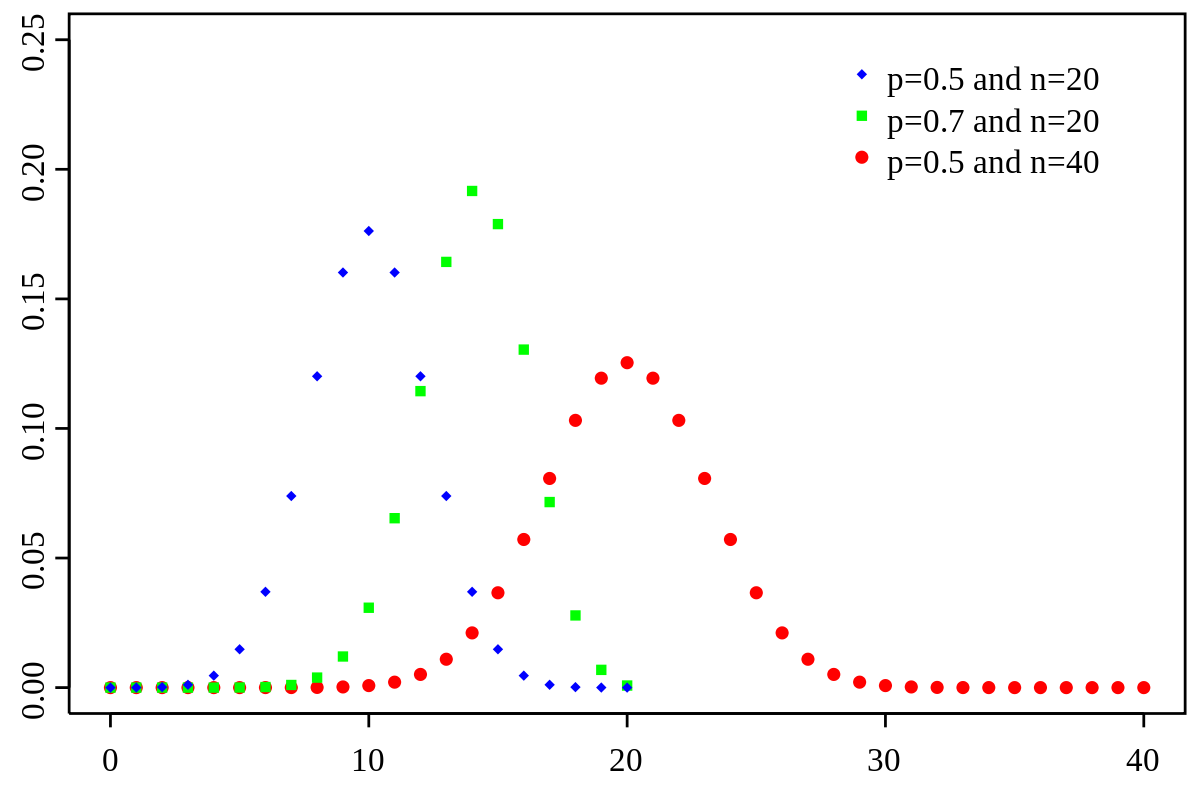
\includegraphics[width=16cm]{Images/Binomial distribution.png}
    \caption{Examples of Binomial Distributions}
    \label{fig:binomial distribution}
\end{figure}

\begin{note}
\end{note}
When $n = 1$, the probability distribution of $X$ becomes $f_X(x) = p^x (1-p)^{1-x},\ x = 0,1$, which is identical to Bernoulli Distribution. Hence, we can say that Bernoulli Distribution is a special case of the binomial distribution. \\
A random variable $X$ is a $B(n,p)$ random variable \textbf{if, and only if,} $X = X_1 + X_2 + \dots + X_n$ where $X_1, \dots , X_n$ are independent random variables, each of which follows the same Bernoulli distribution with the success probability $p$. By convention, we say "$X_1, \dots, X_n$ are independent and identically distributed (i.i.d.) $Bernoulli(p)$ random variables". \\
This is particularly useful to derive the expectation and variance of $X$, as given below.


\thm{Mean and Variance of Binomial Distributions
If $X$ has a binomial distribution with parameters $n$ and $p$ (i.e., $X \sim B(n,p)$), then the mean and variance of $X$ are
\begin{equation*}
\begin{split}
    \mu &= E(X) = np \\
    \sigma^2 &= V(X) = np(1 - p) = npq
\end{split}
\end{equation*}
}
The above formula can be derived by calculating the expected value and variance for each of the individual Bernoulli trial and then adding all of them up. It is always true that if $X = X_1 + X_2 + \dots + X_n$, then $E[X] = E[X_1] + E[X_2] + \dots + E[X_n]$. Moreover since we know that all of $X_1$ through $X_n$ are independent, the covariance of any two of them is zero and so, $V(X) = V(X_1) + V(X_2) + \dots + V(X_n)$. We already know that the expectation for any one trial is $p$ and the variance of any one trial is $pq$ (using Bernoulli trial), hence we easily observe that for $n$ trials, the expectation is $np$ and the variance is $npq$.
\begin{note}[Conditions for a Binomial Experiment]
\end{note}
\begin{enumerate}
    \item It consists of $n$ repeated Bernoulli trials
    \item Only 2 possible outcomes: success and failure in each trial
    \item $P(success) = p$ is the same constant in each trial, i.e., the number of trials previously performed or the outcomes of earlier trials should not affect the probability of success of any trial (e.g. Any experiment "without replacement" is likely to be not a Bernoulli distribution since the successive trials need not be independent). 
    \item Trials are independent
    \item The random variable $X$ is the number of successes among the $n$ trials in a binomial experiment
\end{enumerate}
Only if all the above conditions are met, $X \sim B(n,p)$.

\begin{note}[Derivation of pmf of Binomial distribution]
\end{note}
Consider a specific realization of $X_1, X_2, \dots, X_n$ namely $x_1, x_2, \dots, x_n$ such that $\sum_{i = 1}^n x_i = x$. Note the independence of $X_1, X_2, \dots, X_n$ and that they are all $Bernoulli(p)$ random variables. So, we have,
\begin{equation*}
\begin{split}
    P(X_1 = x_1, X_2 = x_2, \dots, X_n = x_n) &= P(X_1 = x_1)P(X_2 = x_2)\dots P(X_n = x_n) \\
    &= \prod_{i = 1}^{n} p^{x_i}q^{1-x_i} = p^{\sum_{i = 1}^n x_i} q^{n -\sum_{i = 1}^n x_i } \\
    &= p^x q^{n - x}
\end{split}
\end{equation*}
$\sum_{i = 1}^n x_i = x$ on the one hand means that the realized value for the corresponding $X$ is $x$; on the other hand, it means that out of $n$ trials, we get $x$ successes. There are $\binom{n}{x}$ number of such sequences, as we can think of it as choosing $x$ positions to take value 1 out of a length $n$ sequence, and other positions will be 0. As a consequence by nothing that for different choices of $x_1, x_2, \dots , x_n$, $\{X_1 = x_1, X_2 = x_2, \dots , X_n = x_n\}$ are sets of mutually exclusive events, we have
\begin{equation*}
    \begin{split}
        P(X = x) &= P\left( \bigcup_{x_1, \dots, x_n : \sum x_i = x} \{X_1 = x_1, X_2 = x_2 \dots, X_n = x_n \} \right) \\
        &= \sum_{x_1, \dots, x_n : \sum x_i = x} P(X_1 = x_1, X_2 = x_2, \dots, X_n = x_n) \\
        &= \sum_{x_1, \dots, x_n : \sum x_i = x} p^x q^{n-x} = \binom{n}{x}p^x q^{n-x}
    \end{split}
\end{equation*}
\begin{note}
\end{note}
If $X$ and $Y$ are 2 \textbf{independent} random variables that follow Binomial distributions with the same probability of success but possibly differing number of trials, $X + Y$ is also a binomial distribution with the same probability of success but the number of trials equal to the sum of the trials of the two random variables. That is, if $X \sim B(n,p), Y \sim B(m,p)$ then, $ X + Y \sim B(n + m, p)$. (Intuitively this should make sense since they are independent)
\begin{note}[Hypergeometric Distribution]
\end{note}
The hypergeometric distribution is a discrete probability distribution that describes the probability of $k$ successes (random draws for which the object drawn has a specified feature) in $n$ draws, without replacement, from a finite population of size $N$ that contains exactly $K$ objects with that feature, wherein each draw is either a success or a failure. In contrast, the binomial distribution describes the probability of $k$ successes in $n$ draws with replacement. \\
A random variable $X$ follows the hypergeometric distribution if its probability mass function (pmf) is given by:
$$
p_X(k) = P(X = k) = \dfrac{\binom{K}{k}\binom{N - K}{n - k}}{\binom{N}{n}}
$$
where,
\begin{itemize}
    \item $N$ is the population size 
    \item $K$ is the number of success states in the population
    \item $n$ is the number of draws (quantity each trial)
    \item $k$ is the number of observed successes
\end{itemize}

\subsection{Negative Binomial Distribution}
Let us consider an experiment where the properties are the same as those listed for a binomial experiment with the exception that the trials will be repeated until a fixed number of successes occur. \\
We are interested in the probability of the $k^{th}$ success occurring on the $x^{th}$ trial where $x$ is the random variable. Notice how this is different from a binomial distribution in which case we are interested in the probability of $x$ successes in $n$ trials. \\
\begin{definition}[Negative Binomial Distribution] 
Let $X$ be a random variable representing the number of trials to produce the $k$ successes in a sequence of independent Bernoulli trials. The random variable $X$ is said to follow a Negative Binomial Distribution with parameters k and p (i.e. $NB(k,p)$). The probability function of $X$ is given by:
$$
P(X = x) = f_X(x) = 
\begin{cases}
\binom{x-1}{k-1}p^x q^{x-k}, \qquad \text{for } x = k, k + 1, k + 2, ... \\
0, \qquad \text{otherwise}
\end{cases}
$$
\end{definition}
An example of negative binomial distribution would be to find the probability that the 5th success occurs in the 7th trial. So, for this to occur, we need to find the probability of getting 4 successes in the first 6 trials and then multiply that by the probability of getting a success (for the 7th trial).
\thm{Mean and Variance of Negative Binomial Distribution \\
If $X \sim NB(k,p)$, i.e., if $X$ follows a negative binomial distribution with parameters $k$ and $p$, then,
\begin{equation*}
\begin{split}
    \mu &= E[X] = \dfrac{k}{p} \\
    \sigma^2 &= Var(X) = \dfrac{(1-p)k}{p^2}
\end{split}
\end{equation*}
}
\subsection{Geometric Distribution}
A geometric distribution is a special kind of negative binomial distribution in which we find the number of trials required to have the first success. In other words, we set the parameter $k = 1$. So, whenever we talk about a geometric distribution, there is only 1 parameter $p$, which refers to the probability of success for any individual trial. We write $X \sim Geom(0.4)$ to denote that $X$ follows a geometric distribution with probability of success = 0.4. \\
Geometric distribution represents the probability of the number of successive failures before a success is obtained in a Bernoulli trial. That is, in a geometric distribution, a Bernoulli trial is repeated until a success is obtained and then stopped. \\
The probability and cumulative probability functions for a geometric distribution are:
\begin{equation*}
    \begin{split}
        P(X = x) &= p(1-p)^{x-1} \\
        P(X \leq x) &= 1 - (1-p)^x
    \end{split}
\end{equation*}
An easy way to understand the cumulative probability function is to think of the complement event: What is the probability that all the first $x$ trials result in failure? That would be $(1-p)^x$. So, the probability that at least 1 success occurs in the first $x$ trials is just $1 - (1-p)^x$ \\
Obviously, the mean of the geometric distribution is $\dfrac{1}{p}$ and the variance is $\dfrac{1-p}{p^2}$ since $k = 1$.
\begin{note}
\end{note}
Another way to describe a negative binomial distribution is to consider it as the sum of many geometric random variables. For example, $Y \sim NB(k,p)$ and $X_i = Geom(p), i = 1,2,3,\dots, k$. Then, it is possible to write $Y = X_1 + X_2 + \dots + X_k$. So, it follows that $E[Y] = E[X_1] + E[X_2] + \dots E[X_n] = \dfrac{1}{p} + \dfrac{1}{p} + \dots + \dfrac{1}{p} = \dfrac{k}{p}$. Also, $Var(Y) = Var(X_1) + Var(X_2) + \dots + Var(X_k) = \dfrac{1-p}{p^2} + \dfrac{1-p}{p^2} + \dots + \dfrac{1-p}{p^2} = \dfrac{(1-p)k}{p^2}$ 
\section{Poisson Distribution}
\begin{definition}[Poisson Experiments]
Experiments yielding numerical values of a random variable $X$, \textbf{the number of successes occurring during a given time interval or in a specified region}, are called Poisson experiments. They must satisfy the following conditions:
\begin{enumerate}
    \item The number of successes occurring in one time interval or specified region are \textbf{independent} of those occurring in any other disjoint time interval or region of space
    \item The \textbf{probability of a single success} occurring during a very short time interval or in a small region is \textbf{directly proportional to the length of the time interval} or the size of the region and does not depend on the number of successes occurring outside this time interval or region.
    \item The \textbf{probability of more than one success} occurring in such a short time interval or falling in such a small region is \textbf{negligible}.
\end{enumerate}
The given time interval, $t$, may be of any length, such as a minute, a day, a week, or even a year
\end{definition}
Examples of Poisson experiment: generate observations for the random variable $X$ representing the number of telephone calls in an hour received by an office, or the number of postponed games due to rain during a football season. \\
The specified region could be a line segment, an area, a volume, or perhaps a piece of material. In this case, $X$ might represent the number of mushrooms in a plot of land, the number of bacteria in a given culture, or the number of typing errors in a page.

\begin{definition}[Poisson Distribution]
The number of successes $X$ in a Poisson experiment is called a Poisson random variable. The probability distribution of the Poisson random variable $X$, is called the Poisson distribution and the probability function is given by 
$$
f_X(x) = P(X = x) = 
\begin{cases}
\dfrac{e^{-\lambda}\lambda^x}{x!}, \text{ for }x = 0,1,2,3,... \\
0, \text{ otherwise}
\end{cases}
$$
where $\lambda$ is the average number of successes occurring in the given time interval or specified region and $e \approx 2.71828$ is called Euler's number.
\end{definition}
\begin{figure}[ht]
    \centering
    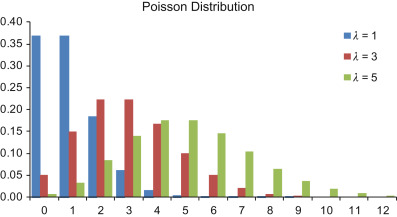
\includegraphics[width = 16cm]{Images/Poisson Distribution.jpg}
    \caption{Example of some Poisson Distributions}
    \label{fig:my_label}
\end{figure}
We write $X \sim P(\lambda)$ to indicate that $X$ follows a Poisson Distribution with parameter $\lambda$.
\thm{Mean and Variance of Poisson Random Variable \\
IF $X$ has a Poisson distribution with parameter $\lambda$, then
\begin{equation*}
    \begin{split}
        \mu &= E[X] = \lambda \\
        \sigma^2 &= V(X) = \lambda
        \end{split}
\end{equation*}}
\begin{note}[Density Manipulation]
\end{note}
The method for deriving these results is called density manipulation. The fundamental idea is simple: for any arbitrary probability function $f(x)$,
\begin{itemize}
    \item if the distribution is discrete, $\sum_{x \in \{x|f(x)>0\}} f(x) = 1$
    \item if the distribution is continuous $\int_{\infty}^{\infty} f(x) = 1$
\end{itemize}
Both of the above follow directly from the axioms of probability (since the total probability must be 1). \\
Proof of mean and variance of Poisson Random Variable:
\begin{equation*}
    \begin{split}
        E(X) &= \sum_{x = 0}^{\infty} x \dfrac{e^{-\lambda}\lambda^x}{x!} \\
        &= \sum_{x = 1}^{\infty} \dfrac{e^{-\lambda}\lambda^x}{(x-1)!} \\
        &= \lambda \sum_{y = 0}^{\infty} \dfrac{e^{-\lambda}\lambda^y}{y!} \qquad \text{where } y = x - 1 \\
        &= \lambda \qquad \text{because } \sum_{y = 0}^{\infty}\dfrac{e^{-\lambda}\lambda^y}{y!} = \sum_{y = 0}^{\infty} f_Y(y) = 1, \text{where } Y \sim P(\lambda) 
    \end{split}
\end{equation*}
In other words, $\sum_{y = 0}^{\infty}\dfrac{e^{-\lambda}\lambda^y}{y!} = 1$ because it is a probability function and its sum over all possible values must be 1. \\
The proof of variance of Poisson Distribution is obtained by first finding $E[X(X - 1)]$.
\begin{equation*}
    \begin{split}
        E[X(X - 1)] &= \sum_{x = 0}^{\infty}x(x-1)\dfrac{e^{-\lambda}\lambda^x}{x!} \\
        &= \sum_{x = 2}^{\infty}\dfrac{e^{-\lambda}\lambda^x}{(x-2)!} \\
        &= \lambda^2 \sum_{y = 0}^{\infty}\dfrac{e^{-\lambda}\lambda^y}{y!} \qquad \text{where } y = x - 2 \\
        &= \lambda^2 \\
        \text{Now, } \\
        V(X) &= E[X^2] - [E(X)]^2 \\
        &= E[X(X - 1)] + E[X] - [E(X)]^2 \qquad \text{due to linearity of expectation}\\
        &= \lambda^2 + \lambda - \lambda^2 \\
        &= \lambda
    \end{split}
\end{equation*}
\begin{note}[Properties of the Poisson Distribution]
\end{note}
\begin{itemize}
    \item Let $X$ follows $Poisson(\lambda_1)$ distribution. Let $Y$ follows $Poisson(\lambda_2)$ distribution. If $X$ and $Y$ are independent, then $X + Y \sim Poisson(\lambda_1 + \lambda_2)$. \\
    For example, if the average number of robberies in a day is 4, then the average number of robberies in 2 days will be 8, assuming that robberies occurring on different days are independent.
    \item Let $X$ be the number of occurrences of an event in a period of time $T$; it has the $Poisson(\lambda)$ distribution. If $Y$ is the number of occurrences of the event in a period of time $tT$, then $Y \sim Poisson(t\lambda)$.
\end{itemize}
\begin{note}[Comparison between Distributions]
\end{note}
Binomial Distribution, Negative Binomial distribution, and the Poisson distribution are all founded on Bernoulli trials. Their corresponding random variables $X$, however are defined differently:
\begin{itemize}
    \item For Binomial distribution, $X$ is defined to be the number of successes out of $n$ independent Bernoulli trials with $p$ constant for all trials.
    \item For Negative Binomial distribution, $X$ is defined to be the number of trials needed so that we achieve $k$ successes.
    \item For Poisson distribution, $X$ is defined to be the number of successes in a period of time or in a specific region.
\end{itemize}

\section{Poisson Approximation to the Binomial Distribution}
\thm{Let $X$ be a \textbf{Binomial} random variable with parameters $n$ and $p$. That is,
$$
P(X = x) = f_X(x) = \binom{n}{x}p^x q^{n-x}, \text{ where } q = 1 - p
$$
Suppose that $n \rightarrow \infty$ and $p \rightarrow 0$ in such a way that $\lambda = np$ remains a constant as $n \rightarrow \infty$. Then, $X$ will have approximately a Poisson distribution with parameter $np$. That is,
$$
\lim_{p \rightarrow 0, \ n \rightarrow \infty}\  P(X = x) = \dfrac{e^{-np}(np)^x}{x!}
$$}
\begin{note}
\end{note}
If $p$ is close to 1, we can still use Poisson distribution to approximate binomial probabilities by interchanging what we have defined to be a success and a failure so that $p$ becomes a value close to zero.
\begin{note}
\end{note}
The reason we can approximate a Binomial distribution using a Poisson distribution because for small values of $p$, the binomial distribution is right skewed (with the right-tail being longer). This makes intuitive sense because the lower the probability of success, the smaller the expected number of successes. Moreover, even the Poisson distribution is right-skewed. On the other hand, when the probability of success is close to $\dfrac{1}{2}$, the binomial distribution becomes nearly symmetric, and hence the normal distribution can better approximate it.

\section{Continuous Uniform Distribution}
\begin{definition}[Continuous Uniform Distribution]
A continuous random variable is said to have a uniform distribution over the interval $[a,b]$, $-\infty < a < b < \infty$, denoted by $U(a,b)$, if its probability density function is given by,
$$
f_X(x) = \begin{cases}
\dfrac{1}{b-a}, \text{ for } a \leq x \leq b \\
0, \text{ otherwise}
\end{cases}
$$
This distribution is also referred to as rectangular distribution because of the rectangular shape of the p.d.f.
\end{definition}
\begin{figure}[ht]
    \centering
    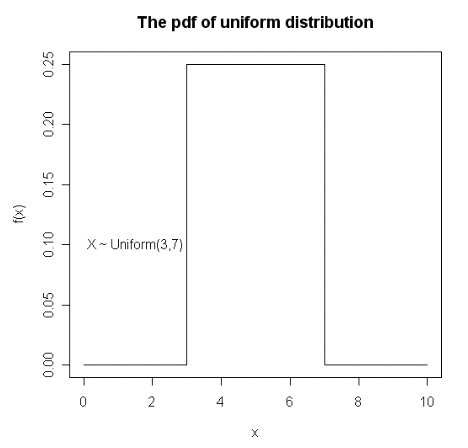
\includegraphics[width = 10cm]{Images/continuous uniform distribution.png}
\end{figure}

\thm{Mean and Variance of Continuous Uniform Distribution \\ 
If $X$ is uniformly distributed over $[a,b]$, then
\begin{equation*}
    \begin{split}
        E[X] &= \dfrac{a + b}{2} \\
        V(X) &= \dfrac{(b-a)^2}{12}
    \end{split}
\end{equation*}
}
Proof:
\begin{equation*}
    \begin{split}
        E[X] &= \int_{a}^{b} x \dfrac{1}{b-a}dx = \dfrac{1}{b-a} \left[ \dfrac{x^2}{2}\right]_{x = a}^{x = b} \\
        &= \dfrac{1}{b-a}\dfrac{b^2 - a^2}{2} \\
        &= \dfrac{a + b}{2} \\
        \text{Also, } \\
        E[X^2] &= \int_{a}^{b} x^2 \dfrac{1}{b-a}dx = = \dfrac{1}{b-a} \left[ \dfrac{x^3}{3}\right]_{x = a}^{x = b} \\
        &= \dfrac{1}{b-a}\dfrac{b^3 - a^3}{3} \\
        &= \dfrac{a^2 + ab + b^2}{3} \\
        \text{Then, } \\
        V(X) &= E[X^2] - (E[X])^2 \\
        &= \dfrac{a^2 + ab + b^2}{3} - \dfrac{(a + b)^2}{4} \\
        &= \dfrac{(b-a)^2}{12}
    \end{split}
\end{equation*}
Keep in mind that these formulae are applicable only when the distribution is defined on a single interval.
\begin{note}[c.d.f. of a uniformly distributed random variable]
\end{note}
Let $X$ be a uniformly distributed random variable between $[a,b]$. Then,
\begin{equation*}
    \begin{split}
        F_X(x) &= \int_{-\infty}^{x} f_X(t)dt \\
        &= \begin{cases}
        \int_{-\infty}^{x} 0 dt, \text{ for } x < a \\
        \int_{-\infty}^{a} 0 dt +  \int_{a}^{x} \dfrac{1}{b-a} dt, \text{ for } a \leq x \leq b \\
        \int_{-\infty}^{a} 0 dt + \int_{a}^{b} \dfrac{1}{b-a} dt + \int_{b}^{x} 0 dt, \text{ for } b < x
        \end{cases} \\
        &= 
        \begin{cases}
        0, \text{ for } x < a \\
        \dfrac{x-a}{b-a} \text{ for } a \leq x \leq b \\
        1, \text{ for } b < x
        \end{cases}
    \end{split}
\end{equation*}

\section{Exponential Distribution}
\begin{definition}[Exponential Distribution]
\end{definition}
A continuous random variable $X$ assuming all non-negative values is said to have an exponential distribution with parameter $\alpha > 0$ if its probability density function is given by
$$
f_X(x) = \begin{cases}
\alpha e^{-\alpha x}, \text{ for } x > 0 \\
0, \text{ otherwise}
\end{cases}
$$
Note that $\int_{-\infty}^{\infty} f_X(x)dx = 1$.

\thm{Mean and Variance of Exponential RV \\ 
If $X$ has an exponential distribution with parameter $\alpha > 0$, then
\begin{equation*}
    \begin{split}
        E[X] &= \dfrac{1}{\alpha} \\
        V(X) &= \dfrac{1}{\alpha^2}
    \end{split}
\end{equation*}}
The proof is very similar to that of continuous uniform distribution and is left an exercise to the reader.

\begin{note}
\end{note}
The p.d.f. can be written in the form $f_X(x) = \dfrac{1}{\mu} e^{\frac{-x}{\mu}}$, for $x > 0$ and 0 otherwise. Then, $E[X] = \mu$ and $V(X) = \mu^2$.

\thm{No Memory Property of Exponential Distribution \\
Suppose that $X$ has an exponential distribution with parameter $\alpha > 0$. Then, for any 2 positive numbers $s,t$, we have
$$
P(X > s + t | X > s) = P(X > t)
$$}
It can be proved using the formulae for conditional probability distributions and is a good exercise for the reader to revise. \\
The above theorem states that the exponential distribution has no memory in the following sense: Let $X$ denote the life length of a bulb. Given that the bulb has lasted $s$ time units (i.e. $X > s$) then the probability that it will last for the next $t$ units (i.e. $X > s + t$) is the same as the probability that it would have lasted for the first $t$ units if it were brand new.\\
This property usually refers to the cases when the distribution of a "waiting time" until a certain event does not depend on how much time has elapsed already. To model memoryless situations accurately, we must constantly 'forget' which state the system is in: the probabilities would not be influenced by the history of the process. For example, assume the bus frequency follows an exponential distribution. If you have been waiting at a bus stop for 10 minutes, what is the probability that you have to wait for 5 more minutes? This probability will be the same for someone who just arrived at the bus stop 10 minutes after you came. So, the expected amount of waiting time does not depend on the time for which you have already been waiting for. \\ Apart from the exponential distribution, the only other distribution which has this memoryless property is the geometric distribution (which makes sense because your odds of getting a success do not increase even though you have performed many trials before it - for example, you toss a coin 3 times and you get tails all 3 times (which you consider to be a failure). Your chances of getting a head (success) remain the same the next time you throw it too).

\begin{note}[c.d.f of the exponential distribution]
\end{note}
Let $X$ be a continuous random variable following an exponential distribution with parameter $\alpha$. Then, for $x \geq 0$,
$$
F_X(x) = P(X \leq x) = \int_{0}^{x} \alpha e^{-\alpha t} dt = \left[-e^{-\alpha t}\right]_{t = 0}^{t = x} = 1 - e^{-\alpha x},
$$ and 0 otherwise. \\
Hence, $P(X > x) = e^{-\alpha x}$, for $x > 0$. \\ \hfill \\
Exponential distribution is popularly used to model the survival (recovery) time of a patient in the medical research, where $P(X > t) = 1 - F_X(t)$ is called the \textbf{survival function} It is the probability that the survival (recovery) time of a patient is greater than $t$.
\begin{note}[Application of the Exponential Distribution]
\end{note}
The exponential distribution is frequently used as a model for the distribution of times between the occurrence of successive events such as customers arriving at a service facility or calls coming into a switchboard.

\section{Normal Distribution}
\begin{definition}[Normal Distribution]
The random variable $X$ assuming all real values, $-\infty < x < \infty$ has a normal (or Gaussian) distribution if its probability density is given by
$$
f_X(x) = \dfrac{1}{\sigma \sqrt{2\pi}} exp\left( - \dfrac{(x-\mu)^2}{2\sigma^2}\right), \text{ for } -\infty < x < \infty
$$ where $-\infty < \mu < \infty $ and $\sigma > 0$.
It is denoted by $N(\mu, \sigma^2)$, and $\mu$ and $\sigma^2$ are called the parameters of the normal distribution.
\end{definition}

\subsection{Properties of the Normal Distribution}
\begin{enumerate}
    \item The graph of this distribution is of bell-shaped and called the normal curve. It is symmetrical about the vertical line $x = \mu$.
    \item The mean, median, and mode of the normal distribution are the same and equal to $\mu$.
    \item The maximum point occurs at $x = \mu$ and its value is $\dfrac{1}{\sigma \sqrt{2\pi}}$.
    \item The normal curve approaches the horizontal axis asymptotically as we proceed in either direction away from the mean.
    \item The total area under the curve and above the horizontal axis is equal to 1 (since it is a probability density function)
    \item It can be shown that $E[X] = \mu$ and $V(X) = \sigma^2$.
    \item 2 normal curves are identical in shape if they have the same $\sigma^2$. But they are centered at different positions when their means are different.
    \item As $\sigma$ increases, the curve flattens, and as $\sigma$ decreases, the curve steepens/sharpens.
    \item If $X \sim N(\mu, \sigma^2)$, and if $Z = \dfrac{X - \mu}{\sigma}$, then $Z \sim N(0,1)$. That is, $Z$ follows the $N(0,1)$ distribution. Then, $E[Z] = 0$ and $V(Z) = 1$. We say that $Z$ has a standardized normal distribution. That is, the p.d.f. of $Z$ may be written as: $f_Z(z) = \dfrac{1}{\sqrt{2\pi}} exp\left( - \dfrac{z^2}{2}\right)$. \\
    The importance of the standardized normal distribution is the fact that it is tabulated. Whenever $X$ has distribution $N(\mu,\sigma^2)$, we can always simplify the process of evaluating the values of $P(x_1 < X < x_2)$ by using the transformation $Z = \dfrac{X - \mu}{\sigma}$. Then,
    $x_1 < X < x_2$ is equivalent to $\dfrac{x_1 - \mu }{\sigma} < Z < \dfrac{x_2 - \mu }{\sigma}$. \\
    Let $z_1 = \dfrac{x_1 - \mu }{\sigma}$ and $z_2 = \dfrac{x_2 - \mu }{\sigma}$. Then, $P(x_1 < X < x_2) = P(z_1 < Z < z_2)$
    \item The density is symmetric about $\mu$, which is the expectation and median of the distribution. One direct consequence is that $P(X \leq \mu) = P(X \geq \mu) = 0.5$. $\mu$ is also called the location parameter, which determines the location of the center of the distribution.
    \item $\sigma^2 = V(X)$ is the shape parameter (also called the dispersion parameter in literature), which determines the shape of the density function.
    \item For any value of $\mu, \sigma^2$, the density if positive for all $x \in \mathbb{R}$. It get closer and closer to (but never equal to) 0, when x approaches $\infty$ or $-\infty$.
    \item The standardization $Z = \dfrac{X - \mu}{\sigma}$ is very important. The density becomes symmetric about 0. That is, for any $z \in \mathbb{R}, \ P(Z \leq -z) = P(Z \geq z)$. $E[Z] = 0$ and $V(Z) = 1$. With this standardization, for $x_1 < x_2$, $P(x_1 < X < x_2)$ (with $\mu$ and $\sigma^2$ being any given values) can always be obtained from the table for $Z$.
    \item For any normal random variable $X$, the probability that $X$ is within $c$ standard deviations from the mean value is always deterministic, where $c > 0$ is a known constant. In particular, if $X \sim N(\mu, \sigma^2)$, 
    $$
    P(\mu - c\sigma < X < \mu + c\sigma) = P(-c < \dfrac{X - \mu}{\sigma} < c) = P(|Z| < c),
    $$ which does not depend on $\mu$ and $\sigma$. Observe that $\dfrac{X - \mu}{\sigma}$ gives you exactly the number of standard deviations that the random variable is away from its expected value.\\
    For example, the probability that a normal random variable is within 1 standard deviation of its mean is 68.27\%, within 2 standard deviations is 95.45\%, and within 3 standard deviations is 99.73\%. So, if the IQ scores of a population follow a normal distribution with mean = 100 and standard deviation = 15, then we can say that 68.27\% of the population has an IQ score between 85 and 115, and 99.73\% of the population has an IQ score between 55 and 145.
    \item For 2 \textbf{independent normal random variables} $X \sim N(\mu_1, \sigma_{1}^2)$ and $Y \sim N(\mu_2, \sigma_{2}^2)$, then $X + Y \sim N(\mu_1 + \mu_2, \sigma_{1}^2 + \sigma_{2}^2)$. Also, $X - Y \sim N(\mu_1 - \mu_2, \sigma_{1}^2 + \sigma_{2}^2)$
\end{enumerate}
\begin{note}
\end{note}
It is important to remember that the last point is not true for any kind of general distribution. For example, if $X \sim exp(\lambda)$ and $Y \sim exp(\lambda)$ and $X$ and $Y$ are independent, $X + Y$ does not follow an exponential distribution.
\begin{figure}[ht]
    \centering
    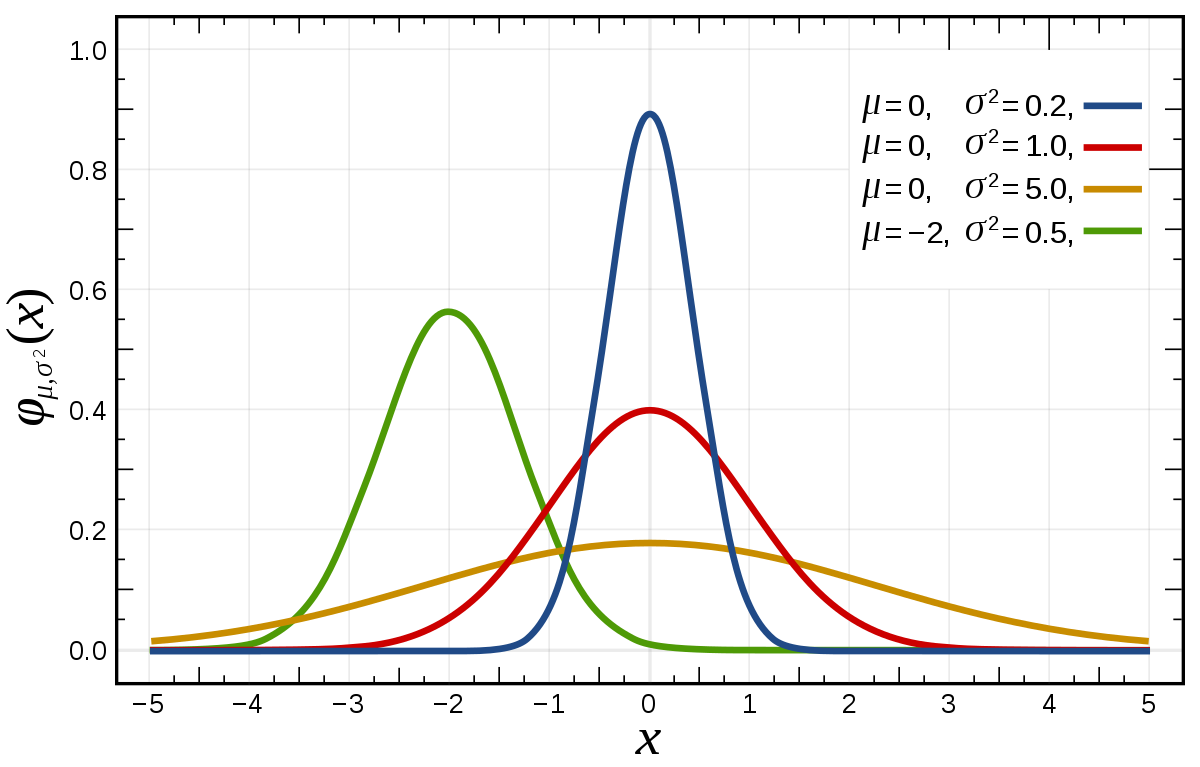
\includegraphics[width = 12cm]{Images/normal.png}
    \caption{Examples of Normal Distribution}
    \label{fig:my_label}
\end{figure}
\subsection{Application of Standardisation}
It is very important to standardise the values before comparing two distributions that follow a normal distribution. The value of $Z$ tells us how far the data point is from the mean (in terms of the number of standard deviations). \\
For example, consider 2 classes - A and B - which had an examination. The distribution of marks in A followed a normal distribution with mean = 50 and standard deviation = 5. Similarly, in class B, the mean was 65 and the standard deviation was 8. Then if student p (from class A) got 60 marks and student q (from class B) got 65 marks, can we say that q is better than p? \\
No! We cannot compare how well p and q did directly without standardising their scores. It may be the case that class B had an easier paper in general or the teacher was lenient. We want to know how well p and q did compared to their class, and use that to determine who did better. So, we find the $Z$ values for both of them, 
$$
Z_p = \dfrac{60 - 50}{5} = 2, \ Z_q = \dfrac{65 - 65}{8} = 0
$$
This can be interpreted as follows: p is 2 standard deviations above the class average (which means he did better than 95\% of his class) while q is average in his class. Hence, we can conclude that p did better than q (assuming that students in both classes are randomly assigned).
\subsection{Statistical Tables}

Statistical tables give the values $\Phi(z)$ for a given $z$, where $\Phi(z)$ is the {\imp {cumulative distribution function of a standardized Normal random variable}} $Z$. It follows that $1 - \Phi(z)$ is the upper cumulative probability for a given $z$. Thus, $\Phi(z) = P(Z \leq z)$ and $1 - \Phi(z) = P(Z > z)$. \\
Some statistical tables give the $100\alpha$ percentage points, $z_\alpha$, of a standardized Normal distribution, where 
$$
\alpha = P(Z \geq z_\alpha) = \int_{z_\alpha}^{\infty}\dfrac{1}{\sqrt{2\pi}} exp \left( - \dfrac{z^2}{2}\right) dz
$$
Since the p.d.f. of $Z$ is symmetrical about 0, $P(Z \geq z_{\alpha}) = P(Z \leq -z_{\alpha}) = \alpha$
\section{Normal Approximation to the Binomial Distribution}
\begin{figure}[ht]
    \centering
    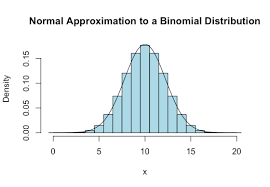
\includegraphics{Images/normal to binomial.png}
\end{figure}
When $n \rightarrow \infty$ and $p \rightarrow 0$, we may use Poisson distribution to approximate a Binomial Distribution. \\
Similarly, when $n \rightarrow \infty$ and $p \rightarrow \dfrac{1}{2}$, we can use normal distribution to approximate the binomial distribution. In fact, even when $n$ is small and $p$ is not extremely close to 0 or 1, the approximation is fairly good. We need $p$ to be close to $\dfrac{1}{2}$ because then the binomial distribution will be close to symmetric and hence, we can approximate it using normal distribution (which is always symmetric). If $p$ is close to 0 or 1, then the binomial distribution is skewed and we cannot use normal distribution to approximate it. Thus, we use Poisson (not symmetric) approximation in such cases. \\
A good rule of thumb is to use the normal approximation only when $np > 5$ and $n(1-p) > 5$.

Notice that we use the Poisson approximation and normal approximation in completely different cases, depending on the value of $p$. If $p$ is close to  0 (or 1), then we use the Poisson approximation. On the other hand, if $p$ is close to $\dfrac{1}{2}$, we use the normal approximation. It is important to keep in mind that these are just approximations and they couldn't give you the exact value. Roughly speaking, how good the approximation is depends on how the corresponding conditions are satisfied.
\thm{If X is a binomial random variable with mean $\mu = np$ and variance $\sigma^2 = np(1-p)$, then as $n \rightarrow \infty$,
$$
Z = \dfrac{X - np}{\sqrt{np(1-p)}} \text{ is approximately } \sim N(0,1)
$$. This is equivalent to saying that $X$ approximately follows $N(np, np(1-p))$ (in the above equation, we have standardized $X$ directly). }
An easy way to remember is that $X$ follows $N(\mu, \sigma^2)$ where $\mu = np$ and $\sigma^2 = np(1-p)$ in the case of binomial distribution. The 2 parameters of the normal distribution always refer to the mean and the variance respectively.
\subsection{Continuity Correction}
\begin{figure}[h]
    \centering
    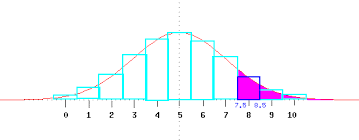
\includegraphics{Images/cont correction.png}
    \caption{Continuity Corrections}
    \label{fig:my_label}
\end{figure}

When we use normal approximation for a binomial distribution to calculate probabilities, we run into some problems. For example, how would we calculate $P(X = k)$ for some value $k$? We know that for a continuous random variable, the probability that $X$ takes on a fixed value is 0. But this is not true for a binomial distribution. Hence, we need to approximate $P(X = k)$ as being equal to $P(k - \dfrac{1}{2} < X < k + \dfrac{1}{2})$. It might be helpful to draw the bars of binomial distribution and the corresponding normal distribution to understand. \\ 
A continuity correction is the name given to adding or subtracting 0.5 to a discrete x-value.
For example, suppose we would like to find the probability that a coin lands on heads less than or equal to 45 times during 100 flips. That is, we want to find $P(X \leq 45)$. To use the normal distribution to approximate the binomial distribution, we would instead find $P(X \leq 45.5)$ because 45 is the midpoint of the bar which ranges from 44.5 to 45.5, and since we want to include the entire bar (since we are including 45), we need to consider the upper bound.
You don't need to memorize this continuity corrections if you understand when to include the point or not and use that to determine whether to add 0.5 or subtract 0.5.
We can use the following approximations in general (only when using normal distribution to approximate binomial distribution):
\begin{enumerate}
    \item $P(X = k) \approx P(k - \frac{1}{2} < X < k + \frac{1}{2})$
    \item $P(a \leq X \leq b) \approx P(a - \frac{1}{2} < X < b + \frac{1}{2})$ \\
    $P(a < X \leq b) \approx P(a + \frac{1}{2} < X < b + \frac{1}{2})$ \\
    $P(a \leq X < b) \approx P(a - \frac{1}{2} < X < b - \frac{1}{2})$ \\
    $P(a < X < b) \approx P(a + \frac{1}{2} < X < b - \frac{1}{2})$
    \item $P(X \leq c) = P(0 \leq X \leq c) \approx P(\frac{-1}{2} < X < c + \frac{1}{2})$ (because the minimum value of  $X$ in a binomial distribution is 0)
    \item $P(X > c) = P(c < X \leq n) \approx P(c + \frac{1}{2} < X < n + \frac{1}{2})$\ (because the maximum value of $X$ in a binomial distribution is $n$)
\end{enumerate}
%\section{Appendix: Statistical Table}
%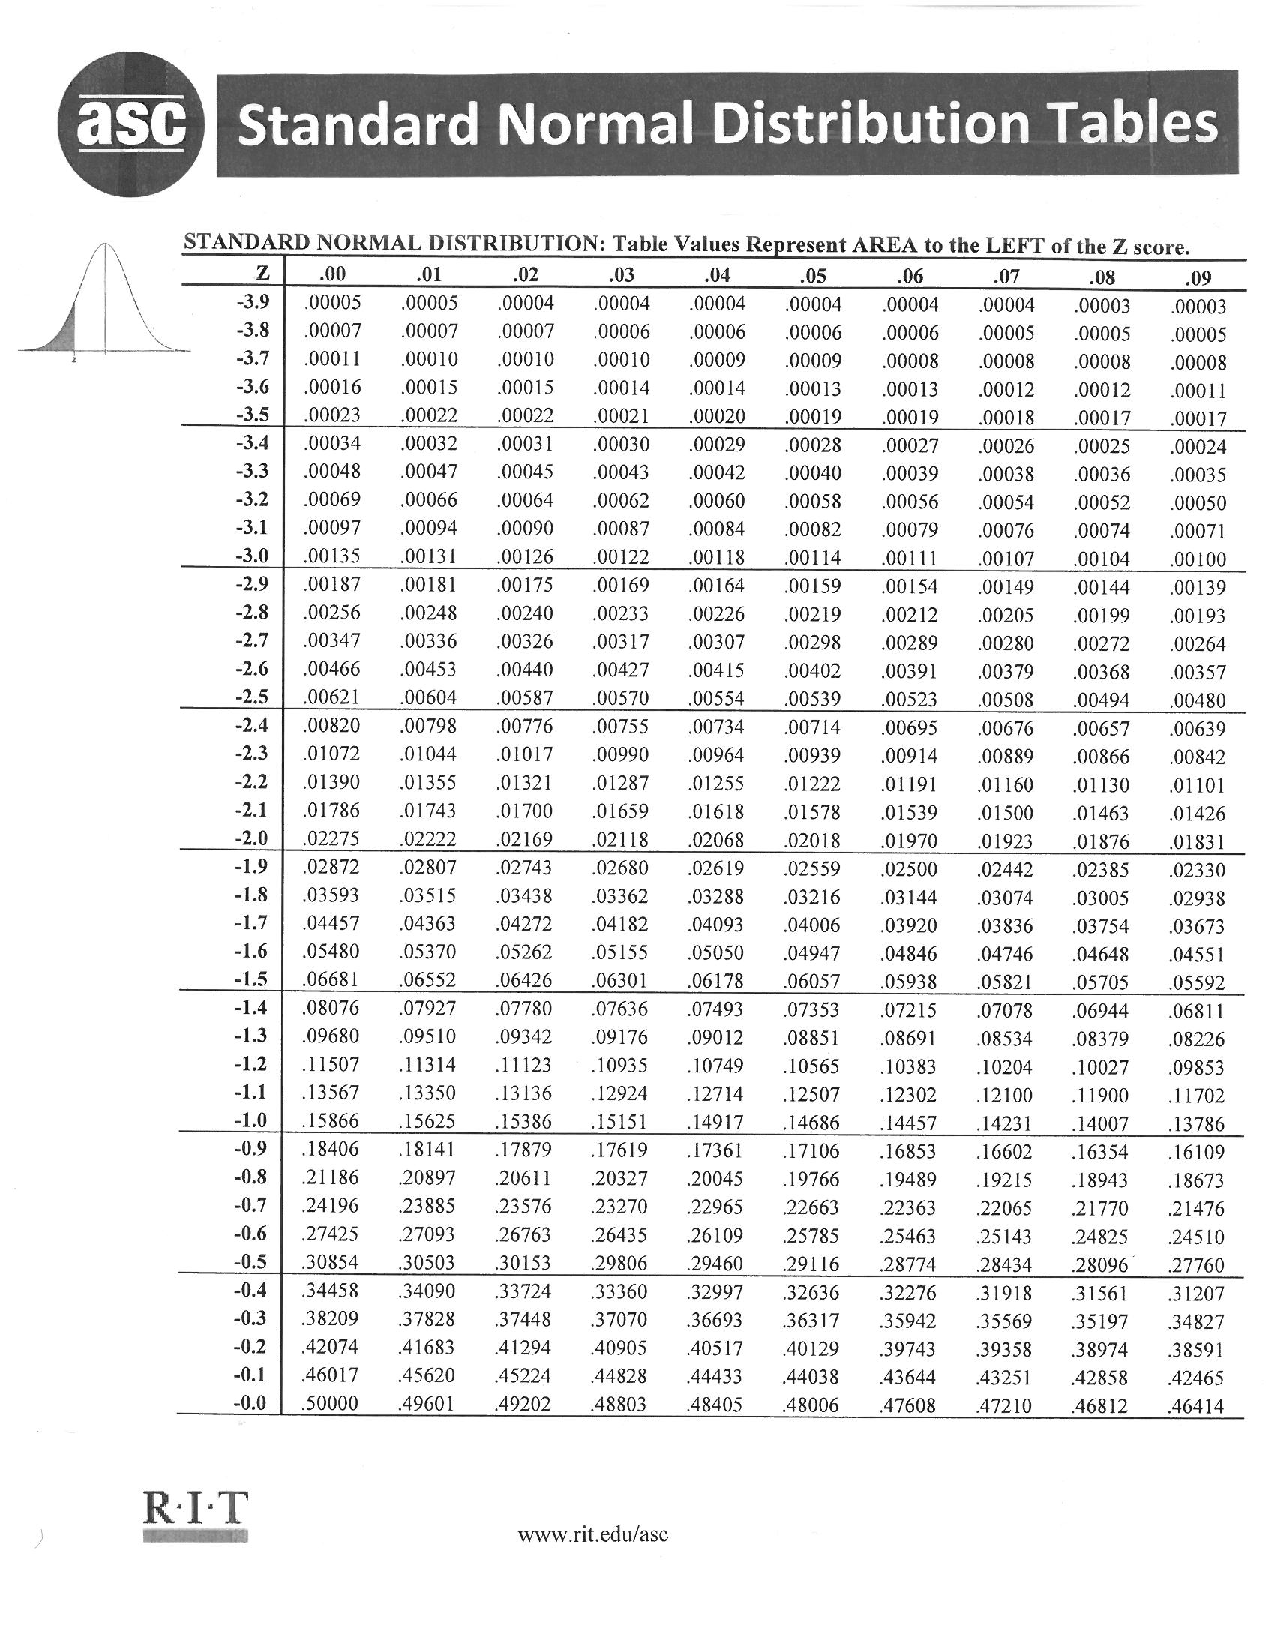
\includepdf[pages=-]{Standard Normal Distribution Table.pdf}

\chapter{Sampling and Sampling Distributions}

\section{Population and Sample}

\begin{definition}[Population]
The totality of all possible outcomes or observations of a survey or experiment is called a population.
\end{definition}
A \textbf{sample} is a subset of a population. \\
Every outcome or observation can be recorded as a numerical or categorical value. Thus, each member of a population is a value of a random variable. There are two kinds of populations, namely, finite and infinite populations.
As the names suggest, a finite population consists of a finite number of elements (for example, the number of species of dogs) whereas an infinite population is one that consists of an infinitely (countable and uncountable) large number of elements (for example, the results of all possible rolls of a pair of dice).

\begin{note}
\end{note}
Some finite populations are so large that in theory we assume them to be infinite, such as the population lives of a certain type of storage battery being manufactured from a factory.

\section{Random Sampling}

\subsection{Simple Random Sampling}
A set of $n$ members taken from a given population is called a \textbf{sample} of size $n$.
\begin{definition}[Simple Random Sample]
A simple random sample of $n$ members is a sample that is chosen in such a way that every subset of $n$ observations of the population has the same probability of being selected. (Or, in other words, each sample point in the population has equal probability of being selected)
\end{definition}
If the process of selecting a sample is \textbf{random}, it is necessarily independent of other samples being drawn.
\subsection{Sampling without Replacement}
In general, there are $\dbinom{N}{n}$ samples of size $n$ that can be drawn from a finite population of size $N$ without replacement (we disregard the order of selection). Each sample has an equal chance of being selected. Hence, each sample has a probability of $\dfrac{1}{\binom{N}{n}}$ of being selected.
\subsection{Sampling with Replacement}
Here, the order of elements is taken into consideration (since 2 elements can appear in the outcome but be chosen in different orders). In general, there are $N^n$ samples of size $n$ that can be drawn from a finite population of size $N$ with replacement.Hence, each sample has a probability of $\dfrac{1}{N^n}$ of being selected
\subsection{Sampling from an Infinite Population (with/without replacement)}
We would be sampling from an infinite population if we sample with replacement from a finite population, and our sample would be random if
\begin{enumerate}
    \item in each draw, all the elements of the population have the same probability of being selected, and
    \item successive draws are independent.
\end{enumerate}
Even if we sample without replacement from an "infinite" population, removing one element from an infinite population does not affect the population. For example, if you have an equal number of infinite red and blue balls. If you draw a red ball in your first draw, the probability of drawing a red ball still remains equal to the blue ball (because you still have infinite red balls!).
\begin{note}
\end{note}
It is important to remember that within a population, there can be many repeated values and each is considered a separate data point. For example, consider the population of all NUS students. Say, we are interested in calculating their CAP. We know that the range of CAP is from 0 - 5 but we don't know the exact CAP of any student prior to sampling. Hence, this is a random variable. Further, multiple students may (in fact by Pigeonhole Principle, must) have the same CAP. We still consider them separate data points since they represent the CAP of different students. Just because the "values" are the same, it does not mean that the data points themselves are the same. 
\begin{note}
\end{note}
Selecting a sample without replacement from a finite population cannot be considered equivalent to sampling from an infinite population since the elements will get exhausted after a finite number of draws. In contrast, for an infinite population or
finite population with replacement, you are able to draw a sample as large as you want.
\begin{definition}[Random Sample]
Let $X$ be a random variable with certain probability distribution, $f_X(x)$. Let $X_1, X_2, \dots , X_n$ be $n$ independent random variables each having the same distribution as $X$, then $(X_1, X_2, \dots, X_n)$ is called a random sample of size $n$ from a population with distribution $f_X(x)$.\\
The joint p.f. (or p.d.f.) of $(X_1, X_2, \dots, X_n)$ is given by $f_{X_1, X_2, \dots, X_n}(x_1, x_2, \dots, x_n) = f_{X_1}(x_1)f_{X_2}(x_2) \dots f_{X_n}(x_n)$, where $f_X(x)$ is the p.f. (or p.d.f.) of the population.
\end{definition}

We say that $(X_1, X_2, \dots, X_n)$ is a random sample from a distribution with probability function $f_X(x)$. Here, a "random sample" is equivalent to  "$X_1, X_2, \dots, X_n$ are independent and identically distributed (i.i.d.)". So, a random sample of size $n$ can be represented by $n$ independent random variables that follow the same distribution. \\
Keep in mind that $X_{i}'s$ follow the same distribution (i.e., identically distributed) does not mean that $X_1 = X_2 = \dots = X_n$ (i.e., identical random variables). \\ You cannot say that $X + Y = 2X$ just because $X$ and $Y$ follow the same distribution. The actual realization of the random variables $X$ and $Y$ may be different even though they follow the same distribution!
Two random variables are equal if, and only if, they map \textbf{each} sample point to the same value. If Alice throws a die and Bob also throws a die, both the outcomes follow the same distribution. But, they are different random variables (if we are interested in the number showing up)! If Alice gets a 4, it does not mean that Bob also gets a 4.
\begin{note}[Motivation behind random sample, parameter, and statistic]
\end{note}
\begin{enumerate}
    \item The population parameter, say, $\mu$,  is \textbf{not observed}; but the values of $X_1, X_2, \dots, X_n$ are observed as $x_1, x_2, \dots, x_n$. So we hope to establish an "estimation rule" to estimate the unknown $\mu$ using the observed $X_1 = x_1, X_2 = x_2 \dots, X_n = x_n$; such a rule is called a statistic (say, $\bar{X} = \dfrac{1}{n}\sum_{i = 1}^n X_i$). In literature, $\bar{X}$ is also called an "estimator" for $\mu$. $\bar{x}$ is \textbf{computed/observed} based on the sample, and is called an estimate.
    \item Note that $\mu$ is an unknown constant - it is not a random variable. The population mean is fixed and constant - we just don't know the value because we haven't got data from the entire population.
    \item The statistic is a function of the sample; the fundamental requirement is that it does not depend on any unknown parameters. for example, $g_1(X_1, \dots, X_n) = 1$ is a statistic since it maps every input of samples to 1. But it is not a useful statistic.
    \item The statistical performance of the statistic decides which one is better to use in practice. In other words, we would be interested in studying the distribution of a statistic, called "sampling distribution". The sampling distribution is also crucial for the subsequent inference for the corresponding parameter.
    \item The sampling distribution for a statistic, say $\bar{X}$, is \textbf{not} how the sample $(X_1, X_2, \dots, X_n)$ performs. Instead, it is the distribution for the corresponding statistic (say, $\bar{X}$). So, constructing the histogram based on the observed $X_1 = x_1, X_2 = x_2, \dots, X_n = x_n$ to have a view of the sampling distribution of $\bar{X}$ is absolutely meaningless. Instead we should do the following:
    \begin{enumerate}
        \item Get the first sample $(X_1^{(1)}, X_2^{(1)}, \dots, X_n^{(1)})$ from the distribution $f_X(x)$, and compute the sample mean $\bar{X}^{(1)}$.
        \item Get the second sample $(X_1^{(3)}, X_2^{(2)}, \dots, X_n^{(2)})$ from the distribution $f_X(x)$, and compute the sample mean $\bar{X}^{(2)}$.
        \item Continue this procedure many times
        \item Get the $K^{th}$ sample $(X_1^{(K)}, X_2^{(K)}, \dots, X_n^{(K)})$ from the distribution $f_X(x)$, and compute the sample mean $\bar{X}^{(K)}$.
        \item Draw the histogram of $\bar{X}^{(1)}, \bar{X}^{(2)}, \dots, \bar{X}^{(n)}$
    \end{enumerate}
    \item In general, $\bar{X} \neq \mu$. $\bar{X}$ is a random variable and can have different realizations depending on the random sample drawn. But, $E[\bar{X}] = \mu$. It is important to understand this difference.
\end{enumerate}

\section{Sampling Distributions of Sample Mean}
Our main purpose in selecting random variables is to elicit information about the unknown population parameters.

\subsection{Statistic and Sampling Distribution}
A function of a random sample $(X_1, X_2, \dots, X_n)$ (which does not depend on any unknown quantities) is called a \textbf{statistic}. For example, $\bar{X}$ is a statistic as $\bar{X} = \dfrac{1}{n} \sum_{i = 1}^n X_i$. \\
Another example is $X_{median}$ or $X_{min}$. \\
But $V = \sum_{i = 1}^n \dfrac{(X_i - \mu)^2}{n - 1}$ is not a statistic if we do not know the population mean.\\
Hence, \textbf{a statistic is a random variable}. It is meaningful to consider the probability distribution of a statistic. The probability distribution of a statistic is called a \textbf{sampling distribution}.
\subsubsection{Sample Mean}
If $X_1, X_2, \dots, X_n$ represent a random sample of size $n$, then the sample mean is defined by the statistic
$$
\bar{X} = \dfrac{1}{n} \sum_{i = 1}^n X_i
$$
If the values in a random sample are observed and they are $x_1, x_2, \dots, x_n$, then the \textbf{realization} of the statistic $\bar{X}$ is given by 
$$\bar{x} = \dfrac{1}{n} \sum_{i = 1}^{n} x_i$$
We denote the population mean by $\mu_X$.

\thm{Sampling Distribution of the sample mean \\
For random samples of size $n$ taken from an infinite population or from a \textbf{finite population with replacement} having population mean $\mu$ and population standard deviation $\sigma$, the sampling distribution of the sample mean $\bar{X}$ has its mean and variance given by 
$$
\mu_{\bar{X}} = \mu_X \qquad \text{and} \qquad  \sigma_{\bar{X}}^2 = \dfrac{\sigma_{X}^2}{n}
$$, where $n$ is the sample size. In other words, 
$$
\mathbb{E}[\bar{X}] = \mathbb{E}[X] \qquad \text{and} \qquad  V(\bar{X}) = \dfrac{V(X)}{n}
$$}

\thm{Law of Large Numbers (LNN) \\
Let $X_1, X_2, \dots, X_n$ be a random sample of size $n$ from a population having any distribution with mean $\mu$ and finite population variance $\sigma^2$. Then for any $\epsilon \in \mathbb{R}$,
$$
P(|\bar{X} - \mu| > \epsilon) \xrightarrow{} 0 \text{ as } n \xrightarrow{} \infty
$$.}
This says that as the sample size increases, the probability that the sample mean differs from the population mean goes to zero. Another way of looking at this is that as $n$ gets larger, it is increasing likely that $\bar{X}$ is close to $\mu$. (The error between our estimated mean and the actual population mean gets smaller and smaller as we conduct sampling with larger and larger samples)
\begin{note}
\end{note}
The strong law of large numbers (also called Kolmogorov's law) states that the sample average converges almost surely to the expected value.
That is, $P(\lim_{n \xrightarrow{} \infty}\bar{X_n} = \mu ) = 1$
\begin{note}[Proof of LLN]
\end{note}
With Chebyshev's inequality, this theorem can be easily proved. Note that $\epsilon$ is an arbitrary but fixed constant. So, we have
$$
0 \leq P(|\bar{X} - \mu| > \epsilon) \leq \dfrac{V(\bar{X})}{\epsilon^2} = \dfrac{\sigma^2}{n \epsilon^2} \xrightarrow{} 0 \qquad \text{as } n \xrightarrow{} \infty
$$
The variance of the population should be finite for the expectation of the random variable $\bar{X}$ to converge to a fixed value. Obviously, $\mu$ must be finite since it is a fixed unknown constant. If variance were infinite,  $\bar{X}$ could assume infinitely many values (realizations) for different random samples and there is no guarantee that the expectation of all these values will be equal to the population mean.

\thm{Central Limit Theorem \\
Let $X_1, X_2, \dots, X_n$ be a random sample of size $n$ from. a population having any distribution with mean $\mu$ and finite population variance $\sigma^2$. The sampling distribution of the sample mean $\bar{X}$ is \textbf{approximately normal} with mean $\mu$ and variance $\dfrac{\sigma^2}{n}$ if $n$ is \textbf{sufficiently large}. Hence, 
$$
Z = \dfrac{\bar{X} - \mu}{\frac{\sigma}{\sqrt{n}}} \text{ follows approximately } N(0,1)
$$}
Note that the variance of the sampling distribution of the sample mean is at most equal to the population variance (since $n \geq 1$). \\
The above theorem is powerful in the sense that it tells us that the distribution of the sampling distribution will be normal if $n$ is large \textbf{no matter what the shape of the population distribution is}.
\begin{enumerate}
    \imp{ \item If for all $i = 1, 2, \dots, n$, $X_i$ are $N(\mu, \sigma^2)$, then $\bar{X}$ follows $N(\mu, \dfrac{\sigma^2}{n})$ regardless of the sample size $n$}
    \item Similarly, if \imp{for all $i = 1, 2, \dots, n$, $X_i$ are approximately $N(\mu, \sigma^2)$, then $\bar{X}$ approximately follows $N(\mu, \dfrac{\sigma^2}{n})$ regardless of the sample size $n$}
\end{enumerate}
Note that the above 2 points have nothing to do with the central limit theorem. With the normality assumption, the distribution of $\bar{X}$ is exactly normal. More generally, the linear combination of independent normal random variables with the same parameters is also a normal random variable (but obviously the parameters change).
If $X_1, X_2, \dots, X_n \sim N(\mu, \sigma^2)$, then $a_1 X_1 + a_2 X_2 + \dots + a_n X_n \sim N(\mu \sum_{i}^n a_i, \sigma^2 \sum_{i}^n a_i^2)$. Then, if you choose each of the $a_i$ to be equal to $\dfrac{1}{n}$, you get the first result.
\begin{note}
\end{note}
Central limit theorem only gives us the approximate distribution for $\bar{X}$, not the exact distribution. More rigorously, central limit theorem says that, for any $z \in \mathbb{R}$, 
$$
\lim_{n \xrightarrow{} \infty} P\left(\dfrac{\bar{X} - \mu)}{\sigma/\sqrt{n}} \leq z \right) = \Phi(z),
$$ where $\Phi(z)$ is the c.d.f. for the standard normal distribution.
So, practically, when $n$ is large, the distribution of $\dfrac{\bar{X} - \mu)}{\sigma/\sqrt{n}}$ is similar to that of a standard normal random variable. We normally use central limit theorem when $n \geq 30$ but this is not a fixed rule. If the actual distribution is quite symmetric, we can use it even for smaller values of $n$. The smaller the $n$, the less accurate the approximation.
\begin{note}
\end{note}
You must ensure that the distribution for which central limit theorem is being applied has a finite variance. For example, a Cauchy distribution has no mean or variance and so you cannot apply the central limit theorem.  Instead, any linear combination of Cauchy variables has a Cauchy distribution (so that the mean of a random sample of observations from a Cauchy distribution has a Cauchy distribution).
\begin{note}[Central Limit Theorem vs LLN]
\end{note}
Central Limit Theorem provides an approximate distribution of $\bar{X}$ (much more information). LLN provides a likely good estimate of $\mu$ based on $\bar{X}$ from a large sample but says nothing about the distribution.
\begin{note}
\end{note}
It is the distribution of $\bar{X}$ that follows approximately a normal distribution if $n$ is large. The underlying distribution of the population does not follow a normal distribution even if $n$ is large, i.e., $\bar{X}$ follows approximately normal as n is large but $X$ does not follow approximately normal even if the population size is very large. Each individual sample still follows the same underlying distribution that the population follows. For example, consider tossing a coin. Let the sample size be 1000. So, one sample consists of tossing a coin 1000 times and noting the number of heads and tails. Find the mean of the sample (assign 1 to head and 0 to tail). Now, repeat this procedure multiple times to get multiple sample means. When looking at the distribution of all the sample means, we expect it to follow a normal distribution but we don't expect each individual sample to follow a normal distribution. In particular, each sample is a Bernoulli distribution (with n = 1000 and p = 0.5). The sample mean is a normal distribution with mean = 0.5 (you are more likely to get 500 heads than 900 heads out of 1000 tosses).

\section{Sampling Distribution of the Difference of 2 Sample means}

\thm{\hfill \\
If independent samples of sizes $n_1$ ($\geq$ 30) and $n_2$ ($\geq$ 30) are drawn from two populations, with means $\mu_1$ and $\mu_2$, and variances $\sigma_1^2$ and $\sigma_2^2$ respectively, then the sampling distribution of the differences of the sample means, $\bar{X_1}$ and $\bar{X_2}$, is approximately normally distributed with mean and variance given by
$$
\mu_{\bar{X_1} - \bar{X_2}} = \mu_1 - \mu_2 \qquad \text{and} \qquad \sigma_{\bar{X_1} - \bar{X_2}}^2 = \dfrac{\sigma_1^2}{n_1} + \dfrac{\sigma_2^2}{n_2}
$$}
The proof the above theorem is relatively straightforward:
$$
\mu_{\bar{X_1} - \bar{X_2}} = E[\bar{X_1} - \bar{X_2}] = E[\bar{X_1}] - E[\bar{X_2}] = \mu_1 - \mu_2
$$
and 
$$
\sigma_{\bar{X_1} - \bar{X_2}}^2 = V(\bar{X_1} - \bar{X_2}) = V(\bar{X_1}) + V(\bar{X_2})
$$
since $\bar{X_1}$ and $\bar{X_2}$ are independent. Therefore, 
$$
\sigma_{\bar{X_1} - \bar{X_2}}^2 = \dfrac{\sigma_1^2}{n_1} + \dfrac{\sigma_2^2}{n_2}
$$
Since $\bar{X_1}$ and $\bar{X_2}$ are approximately normally distributed, therefore $\bar{X_1} - \bar{X_2}$ is also approximately normally distributed.
\begin{note}
\end{note}

\begin{enumerate}
    \item Note that if both $n_1, n_2 \geq 30$, the normal approximation for the distribution of $\bar{X_1} - \bar{X_2}$ is very good regardless of the shapes of the two population distributions.
    \item Recall that if a random variable $Y \sim N(\mu, \sigma^2)$, then $\dfrac{Y - \mu}{\sigma} \sim N(0,1)$. Similarly, here we have
    $$
    \dfrac{(\bar{X_1} - \bar{X_2}) - (\mu_1 - \mu_2)}{\sqrt{\dfrac{\sigma_1^2}{n_1} + \dfrac{\sigma_2^2}{n_2}}} \text{ approximately } \sim N(0,1) 
    $$
\end{enumerate}
We denote the sample standard deviation as $S$ and the sample variance as $S^2$. Further, we denote the population standard deviation as $\sigma$ and population variance as $\sigma^2$.

\section{Chi-Square Distribution}

\begin{definition}[Chi-Square Distribution]
If $Y$ is a random variable  with p.d.f.
$$
f_Y(y) = \begin{cases}
\dfrac{1}{2^{n/2}\Gamma(n/2)} y^{n/2 - 1} e^{-y/2} \text{, for } y > 0 \\
0 \text{, otherwise}
\end{cases}
$$ then $Y$ is said to have a chi-squared distribution with $n$ degrees of freedom, denoted by $\chi^2(n)$, where $n$ is a positive integer, and $\Gamma(.)$ is the gamma function. \\
\end{definition}
The gamma function, $\Gamma(.)$ is defined by 
$$
\Gamma(n) = \int_{0}^{\infty} x^{n-1} e^{-x} dx = (n-1)!
$$ for $n = 1, 2, 3, \dots $
\begin{figure}
    \centering
    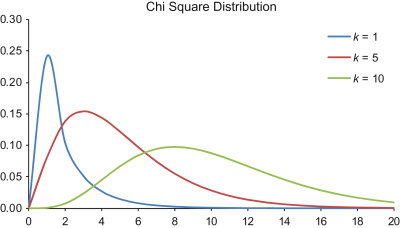
\includegraphics{Images/Chi-squared distribution.jpg}
    \caption{Chi-squared distribution}
    \label{fig:my_label}
\end{figure}
\begin{note}[Some Properties of Chi-square distributions]
\end{note}
\begin{enumerate}
    \item If $Y \sim \chi^2(n)$, then $E[Y] = n$ and $V(Y) = 2n$.
    \item For large $n$, $\chi^2(n)$ approx $\sim N(n,2n)$.
    \item If $Y_1, Y_2, \dots, Y_k$ are \textbf{independent} chi-squared random variables with $n_1, n_2, \dots, n_k$ degrees of freedom respectively, then $Y_1 + Y_2 + \dots + Y_K$ has chi-square distribution with $n_1 + n_2 + \dots + n_k$ degrees of freedom. That is, $\sum_{i = 1}^k Y_i \sim \chi^2 \left( \sum_{i = 1}^k n_i\right)$
\end{enumerate}

\thm{\hfill \\
\begin{enumerate}
    \item If $X \sim N(0,1)$, then $X^2 \sim \chi^2(1)$
    \item Let $X \sim N(\mu, \sigma^2)$, then $[(X - \mu)/\sigma]^2 \sim \chi^2(1)$
    \item Let $X_1, X_2, \dots, X_n$ be a random sample from a normal population with mean $\mu$, and variance $\sigma^2$. Define
    $$
    Y = \sum_{i = 1}^n \dfrac{(X_i - \mu)^2}{\sigma^2}
    $$
    Then $Y \sim \chi^2(n)$
\end{enumerate}}
Let $c$ be a constant satisfying $P(Y \geq c) = \int_{c}^{\infty} f_Y(y) dy = \alpha$, where $Y \sim \chi^2(n)$. We use the notation $\chi^2(n; \alpha)$ to denote this constant $c$. That is, $P(Y \geq \chi^2(n; \alpha)) = \int_{\chi^2(n; \alpha)}^{\infty} f_Y(y) dy = \alpha$. \\
Similarly, $\chi^2(n; 1 - \alpha)$ is the constant satisfying $P(Y \leq \chi^2(n; 1 - \alpha)) = \int_{0}^{\chi^2(n; 1 - \alpha)} f_Y(y)dy = \alpha$

\section{The Sampling Distribution of $(n-1)S^2/\sigma^2$}
Let $X_1, X_2, \dots, X_n$ be a random sample from a population. Then the statistic
$$
S^2 = \dfrac{1}{n - 1} \sum_{i = 1}^n (X_i - \bar{X})^2
$$ is called the sample variance.
The sampling distribution of the random variable $S^2$ has little practical application in statistics. \\
Instead, we shall consider the sampling distribution of the random variable $\dfrac{(n-1)S^2}{\sigma^2}$ when $X_i \sim N(\mu, \sigma^2)$ for all $i$.

\thm{\hfill \\
If $S^2$, is the variance of a random sample of size $n$ taken from a \textbf{normal} population having the variance $\sigma^2$, then the random variable $\dfrac{(n-1)S^2}{\sigma^2}$ has a \textbf{chi-squared distribution with $n - 1$ degrees of freedom.} That is, $\dfrac{(n-1)S^2}{\sigma^2} \sim \chi^2(n-1)$}

\section{The t-distribution}
\begin{figure}
    \centering
    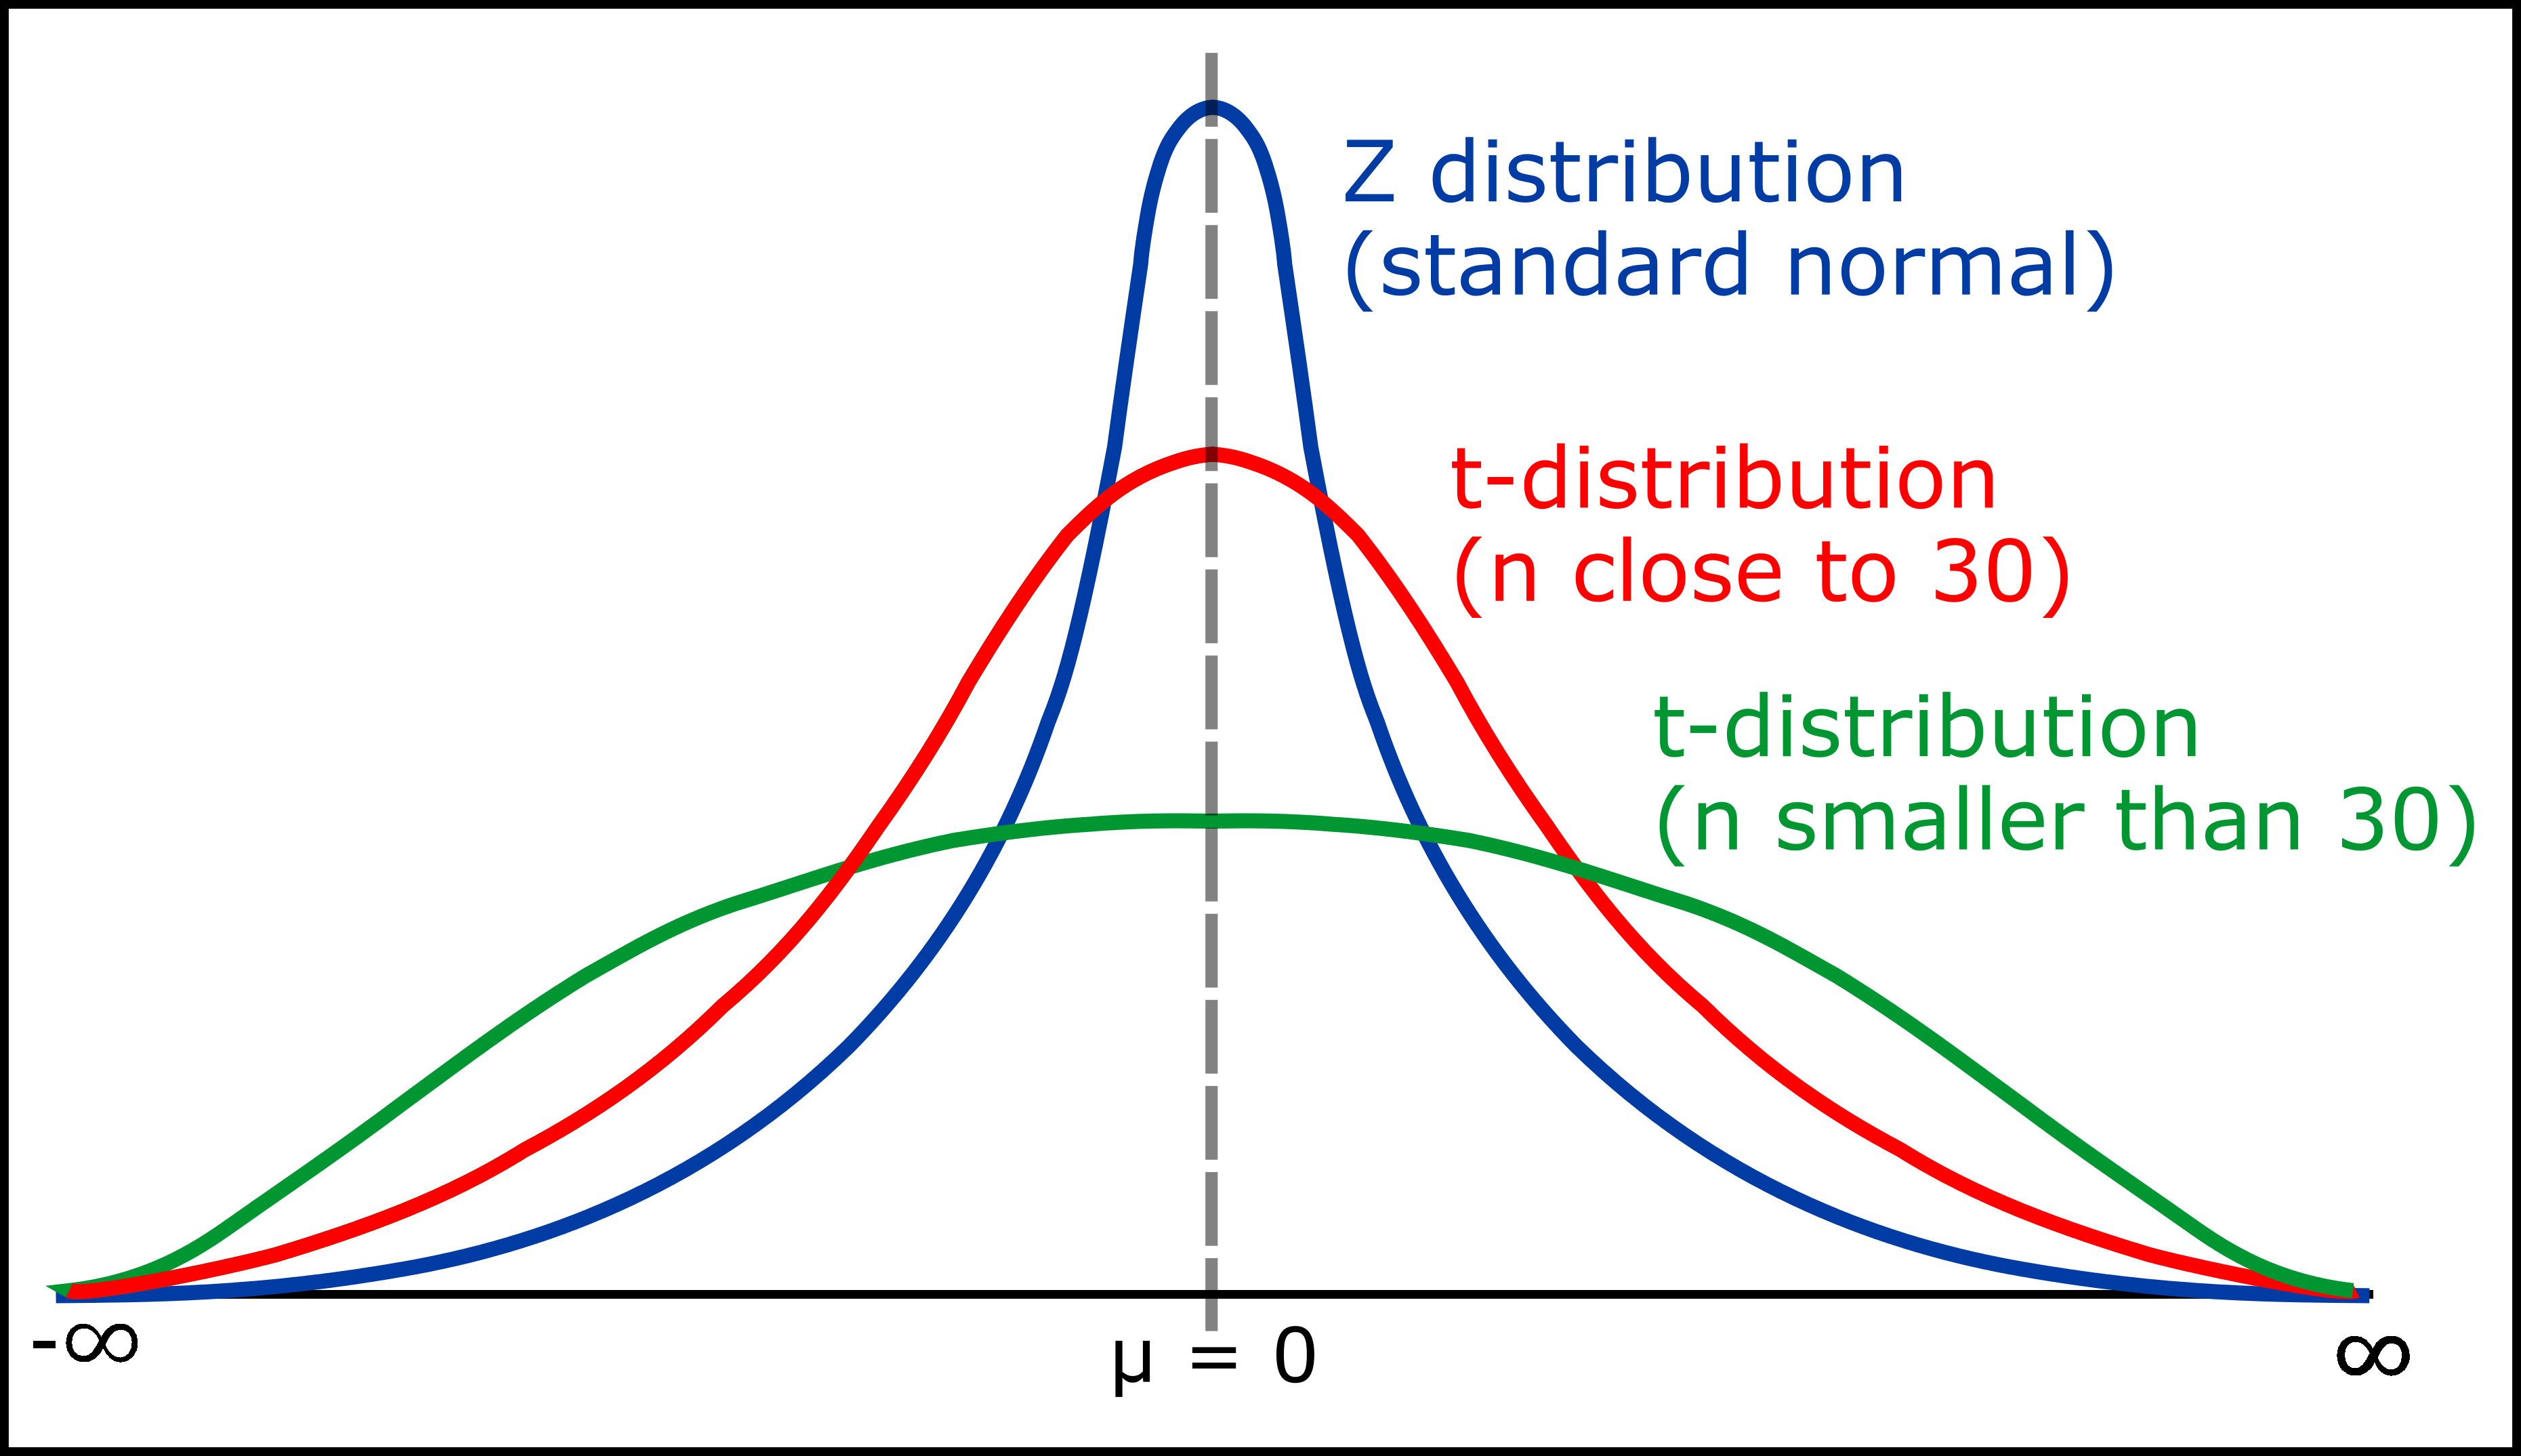
\includegraphics[width = 10cm]{Images/t-distribution.png}
    \caption{t-distribution}
    \label{fig:my_label}
\end{figure}
\begin{definition}[t-distribution]
Suppose $Z \sim N(0,1)$ and $U \sim \chi^2(n)$. If $Z$ and $U$ are \textbf{independent}, and let $T = \dfrac{Z}{\sqrt{U/n}}$ then the random variable $T$ follows the t-distribution with $n$ degrees of freedom. That is, $\dfrac{Z}{\sqrt{U/n}} \sim t(n)$
\end{definition}
If $T$ follows a t-distribution with $n$ degrees of freedom, then its p.d.f. is given by 
$$
f_T(t) = \dfrac{\Gamma \left( \dfrac{n + 1}{2}\right)}{\sqrt{n\pi}\Gamma(n/2)} \left( 1 + \dfrac{t^2}{n}\right)^{\dfrac{n+1}{2}}, \qquad -\infty < t < \infty
$$
where the gamma function is defined as earlier.

\begin{note}
\end{note}
\begin{enumerate}
    \item The graph of the t-distribution is symmetric about the vertical axis and resembles the graph of the standard normal distribution.
    \item It can be shown that the p.d.f. of t-distribution with $n$ d.f. (degrees of freedom) is approaching to the p.d.f. of standard normal distribution when $n \xrightarrow{} \infty$. That is, 
    $$
    \lim_{n \xrightarrow{} \infty} f_T(t) = \dfrac{1}{\sqrt{2\pi}} e^{-t^2 / 2}
    $$ as $n \xrightarrow{} \infty$
    \item The values of $P(T \geq t) = \int_{t}^{\infty} f_T(x) dx$ for selected values of $n$ and $t$ are given in a statistical table.
    \item If $T \sim t(n),$ then $E[T] = 0$ and $V(T) = \dfrac{n}{n - 2}$ for $n > 2$.
\end{enumerate}

\begin{note}
\end{note}
If the random sample was selected from a normal population, then
$$
Z = \dfrac{(\bar{X} - \mu)}{\sigma/\sqrt{n}} \sim N(0,1)
$$ and
$$
U = \dfrac{(n-1)S^2}{\sigma^2} \sim \chi^2(n-1)
$$
It can be shown that $\bar{X}$ and $S^2$ are independent, and so are $Z$ and $U$.
Therefore, 
\begin{equation*}
    \begin{split}
        T &= \dfrac{\bar{X} - \mu }{S/\sqrt{n}} \\
        &= \dfrac{(\bar{X} - \mu)/(\sigma/\sqrt{n})}{\sqrt{\dfrac{(n-1)S^2}{\sigma^2}/(n-1)}} \sim t_{n-1}
    \end{split}
\end{equation*}
That is, $T$ has a t-distribution with $n - 1$ d.f. (degrees of freedom).
Observe the relation between $Z, U, T$ closely. If you replace the $\sigma$ (Population standard deviation) in $Z$ with $S$ (Sample standard deviation), the distribution changes from standard normal to t-distribution with $n - 1$ degrees of freedom.
\section{The F-distribution}
\begin{figure}
    \centering
    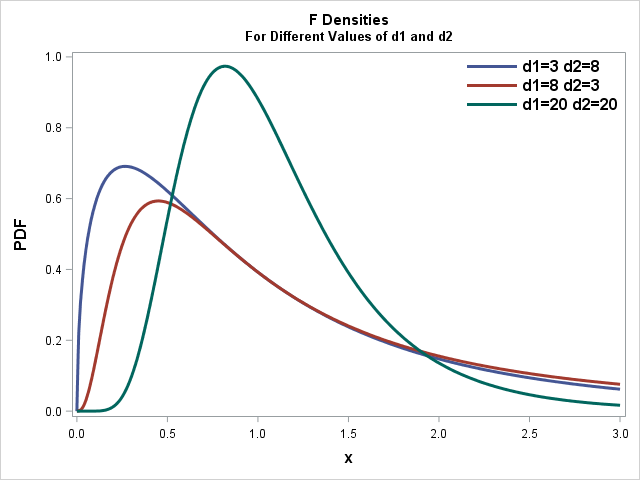
\includegraphics[width = 10cm]{Images/F-distribution.png}
    \caption{F-distribution}
    \label{fig:my_label}
\end{figure}

\begin{definition}[The F-distribution]
Let $U$ and $V$ be independent random variables having $\chi^2(n_1)$ and $\chi^2(n_2)$ respectively. Then, the distribution of the random variable $F = \dfrac{U/n_1}{V/n_2}$, is called a $F$-distribution with $(n_1, n_2)$ degrees of freedom. \\
Observe that $F$ is the ratio of 2 $\chi^2$ random variables, each adjusted by its respective degrees of freedom. Moreover, the parameters of the F-distribution are precisely the degrees of freedom of the 2 $\chi^2$ random variables (first of the random variable in the numerator, then that of the one in the denominator) \\
The p.d.f of $F$ is given by 
$$
f_F(x) = 
\begin{cases}
\dfrac{n_1^{n_1/2}n_2^{n_2/2}\Gamma(\dfrac{n_1 + n_2}{2})}{\Gamma(\dfrac{n_1}{2})\Gamma(\dfrac{n_2}{2})} \dfrac{x^{n_1 / 2 - 1}}{(n_1 x + n_2)^{(n_1 + n_2)/2}}, \text{ for } x > 0 \\
0, \text{ otherwise}
\end{cases}
$$
\end{definition}
It can be shown that 
\begin{equation*}
    \begin{split}
        E[X] &= \dfrac{n_2}{n_2 - 2}, \text{ with } n_2 > 2 \\
        V(X) &= \dfrac{2n_2^2 (n_1 + n_2 - 2)}{n_1(n_2 - 2)^2(n_2 - 4)}, \text{ with } n_2 > 4
    \end{split}
\end{equation*}

\thm{\hfill \\
If $F \sim F(n,m)$, then $\dfrac{1}{F} \sim F(m,n)$}
This theorem follows immediately from the definition of F-distribution. Recall that $F = \dfrac{U/n_1}{V/n_2}$. Then, $\dfrac{1}{F} = \dfrac{V/n_2}{U/n_1}$ follows $F(n_2, n_1)$. \\
Values of the F-distribution can be found in the statistical tables. The table gives the values of $F(n_1, n_2; \alpha)$ such that $P(F > F(n_1, n_2; \alpha)) = \alpha$. For example, $F(5,4; 0.05) = 6.26$ means that $P(F > 6.26) = 0.05$, where $F \sim F(5,4)$.

\thm{
$$
F(n_1, n_2; 1 - \alpha) = \dfrac{1}{F(n_2, n_1; \alpha)}
$$}
Here is a short proof: Let $F \sim F(n_1, n_2)$, then $\dfrac{1}{F} \sim F(n_2, n_1)$, Based on the definition of $F(n_1, n_2; 1 - \alpha)$,
$$
P(F > F(n_1, n_2; 1 - \alpha)) = 1 - \alpha,
$$ which leads to 
$$
P(F < F(n_1, n_2; 1 - \alpha)) = 1 - P(F > F(n_1, n_2; 1 - \alpha)) = \alpha
$$
That is,
$$
P\left(\dfrac{1}{F} > \dfrac{1}{F(n_1, n_2; 1 - \alpha)} \right) = \alpha,
$$
which together with the fact that $\dfrac{1}{F} \sim F(n_2, n_1)$ implies
$$
\dfrac{1}{F(n_1, n_2; 1 - \alpha)} = F(n_2, n_1, \alpha)
$$
\begin{note}
\end{note}
Checking the definition of $t$ and $F$ distributions, we find one important connection between them: If $Y \sim t(n)$, then $Y^2 \sim F(1,n)$
\section{Summary of Sampling Distributions}
\begin{enumerate}
    \item If $X_1, X_2, \dots, X_n$ are $N(\mu, \sigma^2)$, then $\dfrac{\bar{X} - \mu}{\sigma/\sqrt{n}}$ follows $N(0,1)$ regardless of the sample size $n$. If $X_1, X_2, \dots, X_n$ have mean $\mu$ and finite variance $\sigma^2$ and $n$ is sufficiently large, then $\dfrac{\bar{X} - \mu}{\sigma/\sqrt{n}}$ approximately follows the $N(0,1)$ standard normal distribution.
    \item If $X_1, X_2, \dots, X_n$ are $N(\mu, \sigma^2)$, then $\dfrac{(n -1)S^2}{\sigma^2} \sim \chi^2(n-1)$, where $S^2$ is the sample variance of the random sample.
    \item If $X_1, X_2, \dots , X_n$ are $N(\mu, \sigma^2)$, then $\dfrac{\bar{X} - \mu }{S/\sqrt{n}} \sim t(n-1)$.
    \item Let $X_{1,1}, X_{1,2}, \dots, X_{1,n_1}$ be $N(\mu_1, \sigma_1^2)$ and let $X_{2,1}, X_{2,2} \dots, X_{2,n_2}$ be $N(\mu_2, \sigma_2^2)$. Denote by $S_1^2$ and $S_2^2$ the sample variances of $X_{1,1}, X_{1,2}, \dots, X_{1,n_1}$ and $X_{2,1}, X_{2,2} \dots, X_{2,n_2}$ respectively. Then, we have $\dfrac{S_1^2/\sigma_1^2}{S_2^2/\sigma_2^2} \sim F(n_1 - 1 , n_2 - 1)$.
\end{enumerate}

\chapter{Estimation Based on Normal Distribution}

\section{Point Estimation of Mean and Variance}
\subsection{Introduction}
Assume that some characteristics of the elements in a population can be represented by a random variable $X$ whose p.d.f. (or p.f.) is $f_X(x; \theta)$, where the form of the probability density function (or probability function) is assumed known except that it contains an unknown parameter $\theta$. \\
Further assume that the values $x_1, x_2, \dots, x_n$ of a random sample $X_1, X_2, \dots, X_n$ from $f_X(x; \theta)$ can be observed. On the basis of the observed sample values $x_1, x_2, \dots, x_n,$, it is desired to estimate the value of the unknown parameter $\theta$.

\subsection{Estimation}
The estimation can be made in 2 ways: \textbf{Point estimation} and \textbf{Interval estimation}. \\
Point estimation is to let the value of some statistic, say
$$
\hat{\Theta} = \hat{\Theta}(X_1, X_2, \dots, X_n),
$$
to estimate the unknown parameters $\theta$. \\
Such a statistic $\hat{\Theta}(X_1, X_2, \dots, X_n)$ is called a \textbf{point estimator}.\\
Recall that a statistic is a function of the random sample which does not depend on any unknown parameters. Examples of statistic include $\bar{X} = \dfrac{1}{n} \sum_{i = 1}^n X_i$ or $X_{(n)} = max(X_1, X_2, \dots, X_n)$. \\
Let $W = \dfrac{1}{n} \sum_{i = 1}^n (X_i - \mu)^2$. Then $W$ is not a statistic if $\mu$ is not known. However, $W$ is a statistic if $\mu$ is known.

\subsection{Point Estimate of Mean}
Suppose $\mu$ is the population mean. The statistic that one uses to obtain a point estimate is called an estimator. For example, $\bar{X}$ is an estimator of $\mu$. The value of $\bar{X}$, denoted by $\bar{x}$, is an estimate of $\mu$. \\
It should not come as a surprise that different random samples give different point estimates of $\mu$.
\begin{note}
\end{note}
It is important to distinguish clearly these three concepts: an estimator/statistic (e.g. $\bar{X}$), an estimate (e.g. $\bar{x}$), and a population parameter (e.g.$\mu$). An estimator/statistic is a computational rule. It is also a random variable. When the data (random sample) are available, it tells us how to compute. An estimate is a computed value of the estimator based on the observed data (random sample). It is not a random variable - it is a particular realization of the random variable. A population parameter is something about the population - it is not a random variable. Even if you do not know the population parameter, it is an unknown constant, NOT a random variable.

\subsection{Interval Estimation}
Interval estimation is to define two statistics, say, $\hat{\Theta_L}$ and $\hat{\Theta_U}$, where $\hat{\Theta_L} < \hat{\Theta_U}$ so that $(\hat{\Theta_L},\hat{\Theta_U})$ constitutes a random interval for which the probability of containing the unknown parameter $\theta$ can be determined. \\
For example, suppose $\sigma^2$ is known. Let
$$
\hat{\Theta_L} = \bar{X} - 2 \dfrac{\sigma}{\sqrt{n}} \textit{ and } \hat{\Theta_R} = \bar{X} + 2 \dfrac{\sigma}{\sqrt{n}}
$$
Then, $\left(\bar{X} - 2 \dfrac{\sigma}{\sqrt{n}}, \bar{X} + 2 \dfrac{\sigma}{\sqrt{n}} \right)$ is an interval estimator for $\mu$. 
\subsection{Biased and Unbiased Estimators}
\begin{definition}[Unbiased estimator]
A statistic $\hat{\Theta}$ is said to be an unbiased estimator of the parameter $\theta$ if $E[\hat{\Theta}] = \theta$.
\end{definition}
For example, $\bar{X}$ is an unbiased estimator of $\mu$. That is, $E[\bar{X}] = \mu$. \\
Also, $S^2 = \dfrac{1}{n - 1}\sum_{i = 1}^n (X_i - \bar{X})^2$ is an unbiased estimator of $\sigma^2$. That is, $E[S^2] = \sigma^2$. \\
However, $T = \dfrac{1}{n}\sum_{i = 1}^n (X_i - \bar{X})^2$ is a \textbf{biased} estimator of $\sigma^2$.  It can be shown that $E[T] = \dfrac{n-1}{n}\sigma^2 \neq \sigma^2$
\begin{note}
\end{note}
Here is a short derivation for $E[S^2] = \sigma^2$:
\begin{equation*}
    \begin{split}
        \sum_{i = 1}^n (X_i - \bar{X})^2 &= \sum_{i = 1}^n (X_i^2 - 2\bar{X}X_i + \bar{X}^2) \\
        &= \sum_{i = 1}^n X_i^2 - 2 \bar{X} \sum_{i = 1}^n X_i + n\bar{X}^2 \\
        &= \sum_{i = 1}^n X_i^2 - 2n\bar{X}^2 + n\bar{X}^2 \textit{ (because } \bar{X} = \dfrac{\sum_{i = 1}^n X_i}{n} \textit{ )} \\
        &= \sum_{i = 1}^n X_i^2  - n\bar{X}^2 \\
        Now,
        E[S^2] &= E\left[\dfrac{1}{n - 1} \sum_{i = 1}^n (X_i - \bar{X})^2\right] \\
        &= \dfrac{1}{n - 1} E\left[ \sum_{i = 1}^n X_i^2 - n\bar{X}^2\right] \textit{ (based on the result above)} \\
        &= \dfrac{1}{n - 1}\left( E\left[ \sum_{i = 1}^n X_i^2 \right] - n E[\bar{X}^2]\right) \textit{ (linearity of expectation)}\\
        &= \dfrac{1}{n - 1}  \left(\sum_{i = 1}^n E[X_i^2]  - n E[\bar{X}^2] \right) \textit{ (linearity of expectation)} \\
        &= \dfrac{1}{n - 1} \left( \sum_{i = 1}^n[V(X_i) + (E[X])^2] - n[V(\bar{X}) + (E[\bar{X}])^2] \right) \textit{ (because } V(Y) = E[Y^2] - (E[Y])^2 \textit{ )}\\
        &= \dfrac{1}{n - 1} \left ( n \sigma^2 + n\mu^2 - \sigma^2 - n\mu^2 \right ) \textit{ (because } E[X] = \mu, V(X) = \sigma^2, E[\bar{X}] = \mu, V(\bar{X}) = \dfrac{\sigma^2}{n} \textit{ )}\\
        &= \dfrac{1}{n - 1} (n - 1)\sigma^2 \\
        &= \sigma^2
    \end{split}
\end{equation*}
\begin{note}
\end{note}
Let $X_1, X_2, \dots, X_n$ be a random sample. Then, observe that $E(X_1) = \mu$, i.e., $X_1$ is also an unbiased estimator for $\mu$. So, why do we bother to use $\bar{X}$ instead of simply using $X_1$? \\
The answer is quite simple. The variance of $X_1$ is $\sigma^2$. The variance of $\bar{X}$ is $\frac{\sigma^2}{n}$ where $n$ is the sample size. This means that $\bar{X}$ varies less than $X_1$ and so it makes more sense to use that to estimate the population mean. This also provides some intuition as to why the variance of $\bar{X}$ is $\dfrac{\sigma^2}{n}$. We know that $\mu$ is a constant and has variance = 0. So, the larger the sample size, the better the estimate (closer to constant $\mu$) and hence, lower the variability. We're taking the mean of $n$ random variables and so, the variation reduces too.
\begin{note}
\end{note}
Our aim is to find an estimator which is unbiased and has a low variance. But even if a biased estimator has a very low variance, it is not a good estimator. Being unbiased matters more than having low variance. Accuracy (how close your estimate is to the actual value) is more important than precision (how close your estimates are to each other). Consistency matters only when you're actually estimating well. In practice, we choose the estimator with the lowest MSE (Mean Square Error) - We try to minimize the mean of the squares of the error between our estimate and the actual value. For an unbiased estimator, the MSE = variance.
\section{Interval Estimation}
An interval estimate of a population parameter $\theta$ is an interval of the form $\hat{\theta_L} < \theta < \hat{\theta_U}$, where $\hat{\theta_L}$ and $\hat{\theta_U}$ depend on 
\begin{enumerate}
    \item The value of the statistic $\hat{\Theta}$ for the particular sample, and
    \item The sampling distribution of $\hat{\Theta}$
\end{enumerate}
\begin{figure}
    \centering
    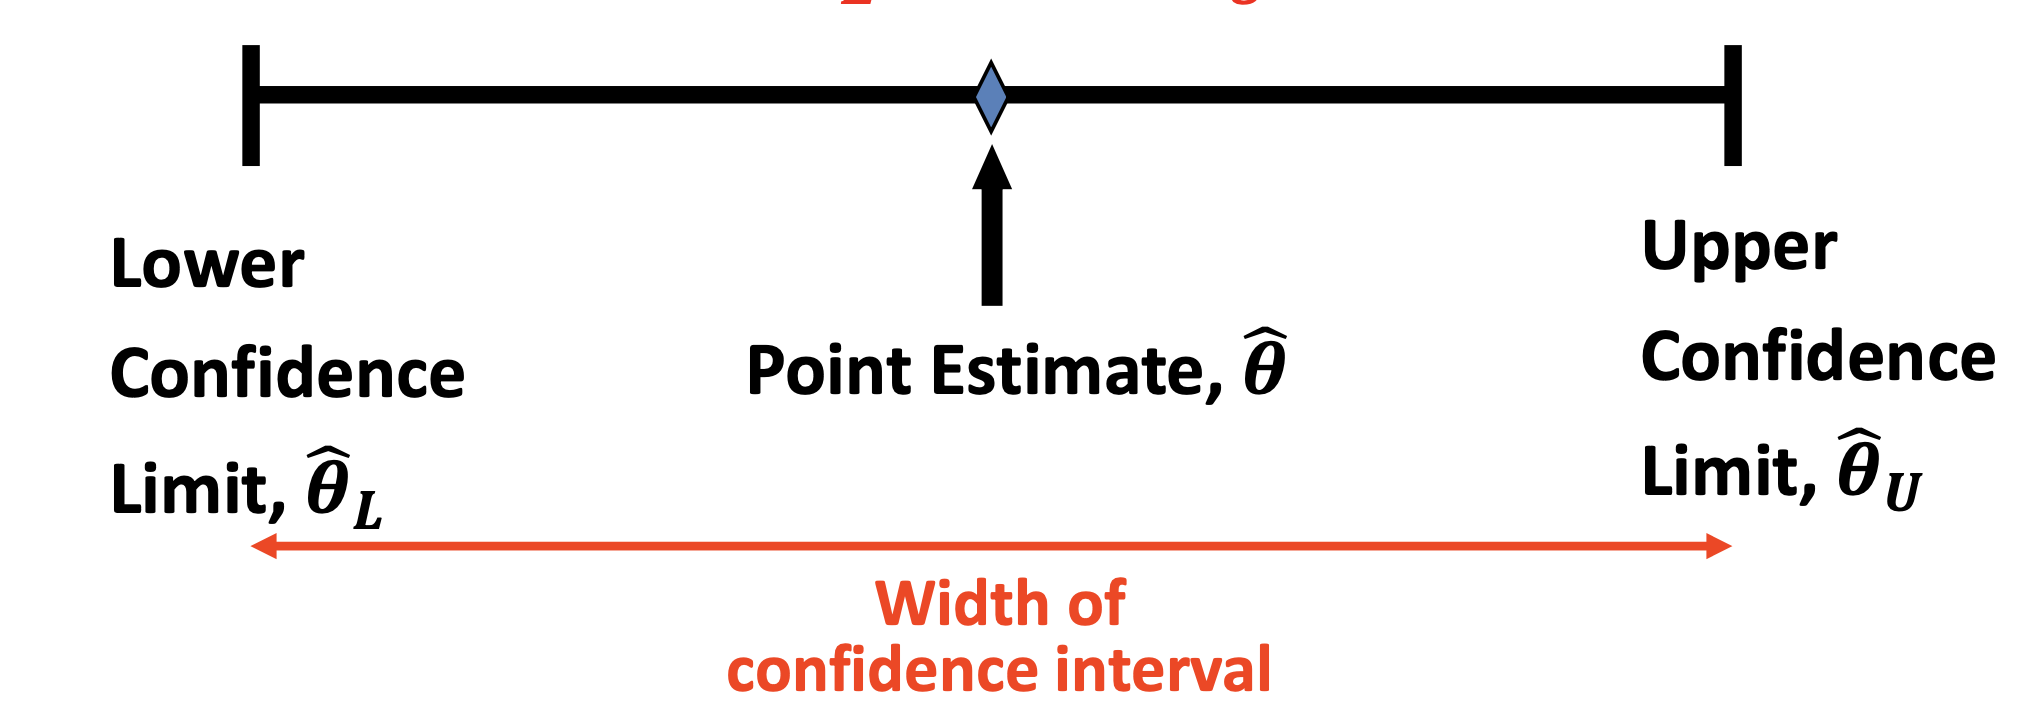
\includegraphics[width = 15cm]{Images/Interval estimation.png}
    \caption{Interval Estimation}
    \label{fig:my_label}
\end{figure}
Since different samples will generally yield different values of $\hat{\Theta}$, and therefore different values of $\hat{\theta_L}$ and $\hat{\theta_U}$, these end points of the interval are values of corresponding random variables $\hat{\Theta_L}$ and $\hat{\Theta_U}$. \\
These intervals may not contain the parameter $\theta$ as $\hat{\theta_L}$ and $\hat{\theta_U}$ vary. \\
We shall seek a random interval $(\hat{\Theta_L}, \hat{\Theta_U})$ containing $\theta$ with a given probability $1 - \alpha$. That is, $P(\hat{\Theta_L} < \theta < \hat{\Theta_U}) = 1 - \alpha$. Then the interval $\hat{\theta_L} < \theta < \hat{\theta_U}$ computed from the selected sample is called a $(1 - \alpha)100\%$ confidence interval for $\theta$ and the fraction $(1 - \alpha)$ is called the \textbf{confidence coefficient} or \textbf{degree of confidence}, and the endpoints $\hat{\theta_L}$ and $\hat{\theta_U}$ are called the lower and upper confidence limits respectively. \\
This means that if samples of the same size $n$ are taken, then in the long run, $(1 - \alpha)100\%$ of the intervals will contain the unknown parameter $\theta$, and hence with a confidence of $(1 - \alpha)100\%$, we can say that the interval covers $\theta$.
\begin{figure}
    \centering
    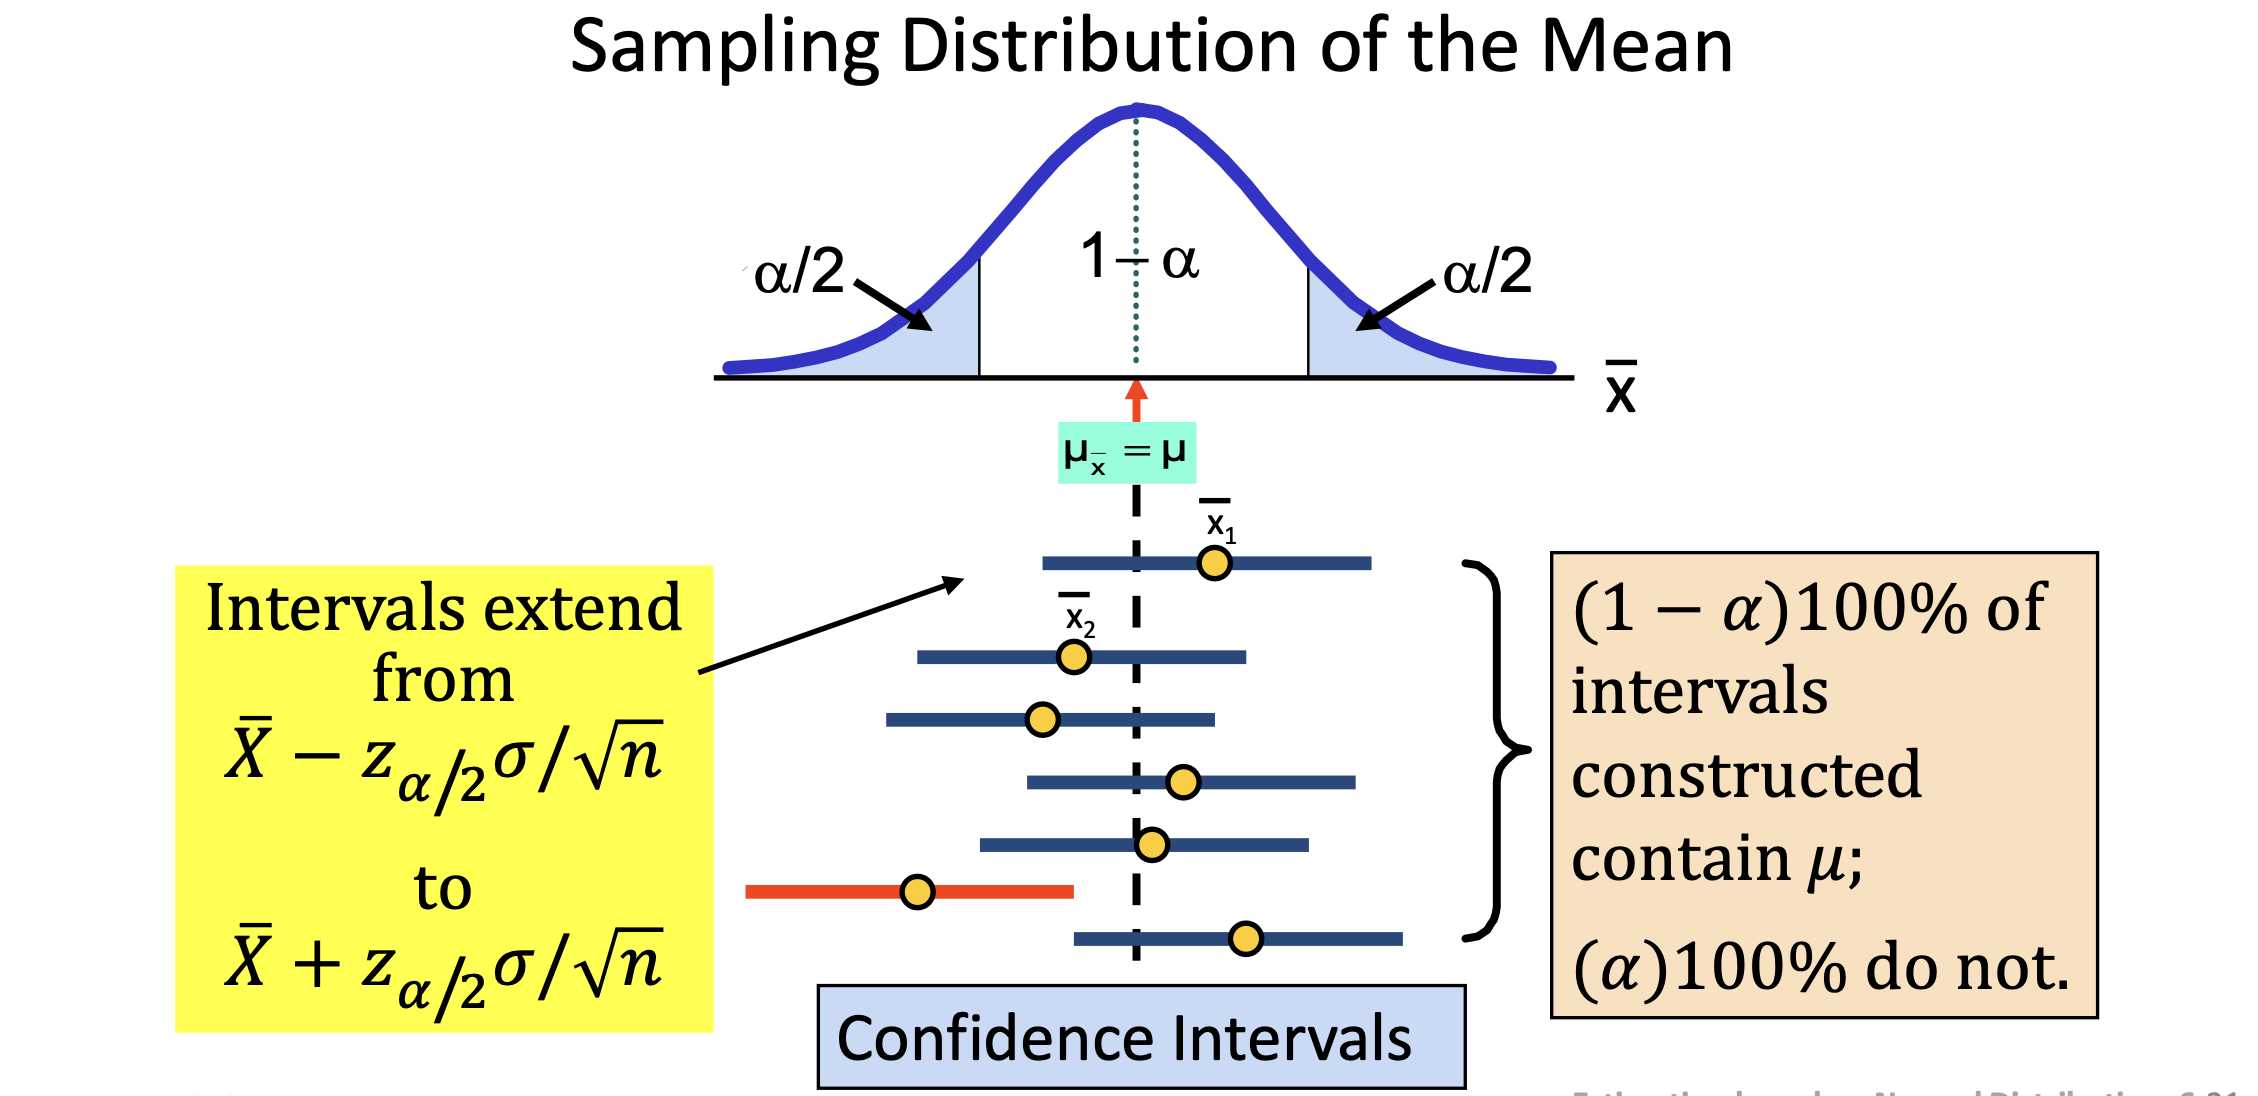
\includegraphics[width = 15cm]{Images/Sampling Distribution of the Mean.png}
    \caption{Sampling Distribution of the Mean}
    \label{fig:my_label}
\end{figure}
\begin{note}
\end{note}
It is important to differentiate the random interval from the interval estimate. Once you have realized the values of the upper and lower bounds of the interval, it does not make sense to talk about the probability of a population parameter lying within the interval. The population parameter is an unknown constant. It either does or does not lie within the computed interval - there is no notion of probability involved. Practically, for a computed C.I., we can only claim that with a certain confidence the interval will cover the true value. This is the reason we choose to say "confidence" rather than "probability"
\section{Confidence Interval (C.I.) for the Mean}
\subsection{Known Variance Case}
Assume that we know the population variance and we are trying to estimate the population mean. Further, we also know that the population distribution is normal or $n$ is sufficiently large (say $n \geq 30)$. \\
Then, by the Central Limit Theorem, we can expect that $\bar{X} \sim N\left(\mu, \dfrac{\sigma^2}{n}\right)$. Therefore, $Z = \dfrac{\bar{X} - \mu }{\sigma/\sqrt{n}} \sim N(0,1)$. Hence,
$$
P\left(-z_{\alpha/2} < \dfrac{\bar{X} - \mu }{\sigma/\sqrt{n}} < z_{\alpha/2}\right) = 1 - \alpha
$$ or
$$
P\left( \bar{X} - z_{\alpha/2}\dfrac{\sigma}{\sqrt{n}} < \mu < \bar{X} + z_{\alpha/2}\dfrac{\sigma}{\sqrt{n}} \right ) = 1 - \alpha
$$
Recall that $P(Z \geq z_{\alpha}) = \alpha$ as per our definition of $z_{\alpha}$. \\
\imp{
Hence, if $\bar{X}$ is the mean of a random sample of size $n$ from a population with known variance $\sigma^2$, a $(1 - \alpha)100\%$ confidence interval for $\mu$ is given by 
$$
\left (\bar{X} - z_{\alpha/2}\dfrac{\sigma}{\sqrt{n}} < \mu < \bar{X} + z_{\alpha/2}\dfrac{\sigma}{\sqrt{n}} \right )
$$}
\subsection{Sampling Size for Estimating $\mu$}
Most of the time, $\bar{X}$ will not be exactly equal to $\mu$ and the point estimate is in error. The size of this error will be $| \bar{x} - \mu |$. We know that 
$P\left( \bar{X} - z_{\alpha/2}\dfrac{\sigma}{\sqrt{n}} < \mu < \bar{X} + z_{\alpha/2}\dfrac{\sigma}{\sqrt{n}} \right ) = 1 - \alpha$. In other words, 
$$
P\left( |\bar{X} - \mu | < z_{\alpha/2} \dfrac{\sigma}{\sqrt{n}}\right) = 1 - \alpha
$$
Let $e$ denote the margin of error. We want the error $|\bar{X} - \mu |$ does not exceed the margin of error, $e$, with a probability larger than $1 - \alpha$. That is,
$$
P(|\bar{X} - \mu | \leq e) \geq 1 - \alpha
$$
Since $P\left( |\bar{X} - \mu | < z_{\alpha/2} \dfrac{\sigma}{\sqrt{n}}\right) = 1 - \alpha$, therefore
$$
e \geq z_{\alpha/2} \dfrac{\sigma}{\sqrt{n}}
$$
Hence for a given margin of error $e$, the sample size is given by
\imp{
$$
n \geq \left( z_{\alpha/2}\dfrac{\sigma}{e} \right)^2
$$}
\begin{note}
\end{note}
It is important to understand the implications of the above formula. The required sample size depends on:
\begin{enumerate}
    \item $z_{\alpha/2}$ (and hence on $\alpha$). In particular, lower the value of $\alpha$, higher the value of $z_{\alpha/2}$. So, for a higher degree of confidence, we need to have a larger sample size (as expected)
    \item $\sigma$ - If the underlying distribution shows higher variation, it is necessary to have a larger sample size to have the same margin of error and degree of confidence.
    \item $e$ - To have a lower margin of error, you need to have a higher sample size.
\end{enumerate}
\subsection{Unknown Variance Case}
We now try to find the confidence interval for mean with:
\begin{enumerate}
    \item unknown population variance
    \item the population is normal or very close to normal distribution
    \item the sample size is small (so we cannot use central limit theorem)
\end{enumerate}
Let $T = \dfrac{\bar{X} - \mu }{S/\sqrt{n}}$ where $S^2$ is the sample variance. We know that $T \sim t_{n-1}$. Hence, 
\begin{equation*}
    \begin{split}
        P\left( -t_{n - 1; \alpha/2} < T < t_{n-1; \alpha/2} \right) &= 1 - \alpha \\
        P\left( -t_{n - 1; \alpha/2} < \dfrac{\bar{X} - \mu }{S/\sqrt{n}} < t_{n-1; \alpha/2} \right) &= 1 - \alpha \\
        P\left( -t_{n - 1; \alpha/2}\dfrac{S}{\sqrt{n}} < \bar{X} - \mu < t_{n-1; \alpha/2}\dfrac{S}{\sqrt{n}}  \right) &= 1 - \alpha \\
        P\left(\bar{X} - t_{n - 1; \alpha/2}\dfrac{S}{\sqrt{n}} < \mu <\bar{X} + t_{n-1; \alpha/2}\dfrac{S}{\sqrt{n}}  \right) &= 1 - \alpha \\
    \end{split}
\end{equation*}

\imp{So, If $\bar{X}$ and $S$ are the sample mean and the standard deviation of a random sample of size $n < 30$ from an approximate normal population with unknown variance $\sigma^2$, a $(1 - \alpha)100\%$ confidence interval for $\mu$ is given by 
$$
\bar{X} - t_{n - 1; \alpha/2}\dfrac{S}{\sqrt{n}} < \mu <\bar{X} + t_{n-1; \alpha/2}\dfrac{S}{\sqrt{n}}
$$

For large $n$ (say, $n > 30$), the t-distribution is approximately the same as the $N(0,1)$ distribution. Hence, we can replace $t_{n-1; \alpha/2}$ by $z_{\alpha/2}$. So, when $\sigma^2$ is unknown, population is normal and $n > 30$, a $(1-\alpha)100\%$ confidence interval is given by 
$$
\bar{X} -z_{\alpha/2}\dfrac{S}{\sqrt{n}} < \mu <\bar{X} + z_{\alpha/2}\dfrac{S}{\sqrt{n}}
$$}
\section{Confidence Intervals (C.I.) for the Difference between 2 Means}
If we have 2 populations with means $\mu_1$ and $\mu_2$ and variances $\sigma_1^2$ and $\sigma_2^2$ respectively, then $\bar{X_1} - \bar{X_2}$ is the point estimator of $\mu_1 - \mu_2$.
\subsection{Known Variances}
If $\sigma_1^2$ and $\sigma_2^2$ are known and not equal, and the two populations are normal, or when $\sigma_1^2$ and $\sigma_2^2$ are known and not equal but $n_1, n_2$ are sufficiently large ($n_1 \geq 30, n_2 \geq 30$), then we know that
$$
(\bar{X_1} - \bar{X_2}) \sim N\left (\mu_1 - \mu_2, \dfrac{\sigma_1^2}{n_1} + \dfrac{\sigma_2^2}{n_2}\right)
$$
\imp{
We can assert that
$$
P
\left( -z_{\alpha/2} < \dfrac{(\bar{X_1} - \bar{X_2}) - (\mu_1 - \mu_2)}{\sqrt{\dfrac{\sigma_1^2}{n_1} + \dfrac{\sigma_2^2}{n_2}}} < z_{\alpha/2}
 \right) = 1 - \alpha
$$
which leads to the following $(1-\alpha)100\%$ confidence interval for $\mu_1 - \mu_2$
$$
(\bar{X_1} - \bar{X_2}) - z_{\alpha/2} \sqrt{\dfrac{\sigma_1^2}{n_1} + \dfrac{\sigma_2^2}{n_2}} < \mu_1 - \mu_2 < (\bar{X_1} - \bar{X_2}) + z_{\alpha/2} \sqrt{\dfrac{\sigma_1^2}{n_1} + \dfrac{\sigma_2^2}{n_2}}
$$
}
\subsection{Large Sample Confidence Interval (C.I.) for Unknown Variances}
We use this when:
\begin{enumerate}
    \item $\sigma_1^2$ and $\sigma_2^2$ are unknown
    \item $n_1, n_2$ are sufficiently large ($n_1 \geq 30, n_2 \geq 30$)
    \item We may replace $\sigma_1^2$ and $\sigma_2^2$ by their estimates $S_1^2$ and $S_2^2$
\end{enumerate}
Then, a $(1-\alpha)100\%$ confidence interval for $\mu_1 - \mu_2$ is given by:
$$
(\bar{X_1} - \bar{X_2}) - z_{\alpha/2} \sqrt{\dfrac{S_1^2}{n_1} + \dfrac{S_2^2}{n_2}} < \mu_1 - \mu_2 < (\bar{X_1} - \bar{X_2}) + z_{\alpha/2} \sqrt{\dfrac{S_1^2}{n_1} + \dfrac{S_2^2}{n_2}}
$$

\subsection{Unknown but Equal Variances}
We use this when:
\begin{enumerate}
    \item $\sigma_1^2$ and $\sigma_2^2$ are unknown but equal
    \item The two populations are normal
    \item Sample sizes are small ($n_1 \leq 30, n_2 \leq 30$)
\end{enumerate}
Let $\sigma_1^2 = \sigma_2^2 = \sigma^2$, then
$$
(\bar{X_1} - \bar{X_2}) \sim N\left( \mu_1 - \mu_2, \sigma^2\left(\dfrac{1}{n_1} + \dfrac{1}{n_2} \right) \right)
$$
Therefore we obtain a standard normal random variable in the form
$$
Z = \dfrac{\bar{X_1} - \bar{X_2} - (\mu_1 - \mu_2)}{\sqrt{\sigma^2 \left( \dfrac{1}{n_1} + \dfrac{1}{n_2} \right)}}
$$
\imp {We can estimate $\sigma^2$ by the pooled sample variance (essentially just taking the weighted average):
$$
S_p^2 = \dfrac{(n_1 - 1)S_1^2 + (n_2 - 1)S_2^2}{n_1 + n_2 - 2}
$$
where $S_1^2$ and $S_2^2$ are the sample variances of the first and second samples respectively.} \\
Remember that $S_p^2$ is an estimator for the population variance, and NOT an estimator for the variance of the difference of the means. To get an estimate for the variance of the difference of the means, you still need to multiply $S_p^2$ by $\left(\dfrac{1}{n_1} + \dfrac{1}{n_2}\right)$
\begin{note}
\end{note}
The above formula should intuitively make sense: every observation contributes equally in the estimation of their common variance $\sigma^2$. In terms of samples, it is the weighted average of the 2 sample variances with the weights being one less than the sample sizes. \\
Note that if the two populations are normal with the same variance $\sigma^2$, then $\dfrac{(n_1 - 1)S_1^2}{\sigma^2} \sim \chi_{n_1 - 1}^2$ and $\dfrac{(n_2 - 1)S_1^2}{\sigma^2} \sim \chi_{n_2 - 1}^2$. \\
Hence, 
$$
\dfrac{(n_1 - 1)S_1^2 + (n_2 - 1)S_2^2}{\sigma^2} \sim \chi_{n_1 + n_2 - 2}^2
$$
Substituting $S_p^2$ for $\sigma^2$, we obtain the statistic:
$$
T = \dfrac{(X_1 - X_2) - (\mu_1 - \mu_2)}{\sqrt{S_p^2 \left( \dfrac{1}{n_1} + \dfrac{1}{n_2} \right)}} \sim t_{n_1 + n_2 - 2}
$$
We can assert that
$$
P\left( -t_{n_1 + n_2 - 2; \alpha/2} <   \dfrac{(X_1 - X_2) - (\mu_1 - \mu_2)}{\sqrt{S_p^2 \left( \dfrac{1}{n_1} + \dfrac{1}{n_2} \right)}} < t_{n_1 + n_2 - 2; \alpha/2} \right) = 1 - \alpha
$$
\imp{Therefore a $(1 - \alpha)100\%$ confidence interval for $\mu_1 - \mu_2$ is given by:
$$
(\bar{X_1} - \bar{X_2}) -t_{n_1 + n_2 - 2; \alpha/2}S_p \sqrt{\dfrac{1}{n_1} + \dfrac{1}{n_2}} < \mu_1 - \mu_2 < (\bar{X_1} - \bar{X_2}) + t_{n_1 + n_2 - 2; \alpha/2}S_p \sqrt{\dfrac{1}{n_1} + \dfrac{1}{n_2}}
$$
where $S_p$ is the pooled estimate of the population standard deviation and $t_{n_1 + n_2 - 2; \alpha/2}$ is the value from the t-distribution with the degrees of freedom $n_1 + n_2 - 2$ leaving an area of $\alpha/2$ to the right. In other words, $P(W > t_{n_1 + n_2 - 2; \alpha/2}) = \alpha/2$ where $W \sim t_{n_1 + n_2 - 2}$.}

\subsection{C.I. for the difference between 2 means for paired data (dependent data)}
Say for example, we run a test on a new diet using 15 individuals, the weights before ($x_i$) and after ($y_i$) the completion of the diet form our two samples. Observations in the two samples made on the same individual are related and hence, form a pair. To determine if the diet is effective, we must consider the differences $d_i = x_i - y_i$ of paired observations. \\
These differences are the values of the random sample $d_1, d_2, \dots, d_n$ from a population that we shall assume to be normal with mean $\mu_D$ and unknown variance $\sigma_D^2$. In fact, $\mu_D  = \mu_1 - \mu_2$ (by linearity) and the point estimate of $\mu_D$ is given by 
$$
\bar{d} = \dfrac{1}{n} \sum_{i = 1}^n d_i = \dfrac{1}{n} \sum_{i = 1}^n (x_i - y_i)
$$. 
The point estimate of $\sigma_D^2$ is given by 
$$
S_D^2 = \dfrac{1}{n - 1} \sum_{i = 1}^n (d_i - \bar{d})^2
$$
For a small sample and approximately normal population, a $(1 - \alpha)100\%$ confidence interval for $\mu_D$ can be established as follows:
$$
P(-t_{n - 1; \alpha/2} < T < t_{n - 1; \alpha/2}) = 1 - \alpha
$$ where $T = \dfrac{\bar{d} - \mu_D}{S_D / \sqrt{n}} \sim t_{n -1}$\\
\imp{
Therefore, a $(1 - \alpha)100\%$ confidence interval for $\mu_D = \mu_1 - \mu_2$ is given by:
$$
\bar{d} - t_{n - 1; \alpha/2}\dfrac{S_D}{\sqrt{n}} < \mu_D < \bar{d} + t_{n - 1; \alpha/2}\dfrac{S_D}{\sqrt{n}}
$$
For a large sample ($n > 30$), we may replace $t_{n-1; \alpha/2}$ by $z_{\alpha/2}$ and a $(1 - \alpha)100\%$ confidence interval for $\mu_D = \mu_1 - \mu_2$ is given by:
$$
\bar{d} - z_{\alpha/2}\dfrac{S_D}{\sqrt{n}} < \mu_D < \bar{d} + z_{ \alpha/2}\dfrac{S_D}{\sqrt{n}}
$$}
\begin{note}
\end{note}
{\color{blue} Here is a general strategy for constructing mean related confidence intervals. Suppose we are to construct a $(1 - \alpha)$ confidence interval for mean related parameter $\theta$ (e.g. $\theta$ could be $\mu$, $\mu_1 - \mu_2$, or other possible combinations of the population means). Then, the following are the steps you need to follow:
\begin{enumerate}
    \item Look for an estimator $\hat{\theta}$ for $\theta$, e.g. $\bar{X}$ for $\mu$, $\bar{X_1} - \bar{X_2}$ for $\mu_1 - \mu_2$.
    \item Derive the variance $V(\hat{\theta})$.
    \item Construct $(1 - \alpha)$ C.I. to be $\hat{\theta} \pm M \sqrt{V}$ where $M$ is called the multiplier, and $V$ is related to $V(\hat{\theta})$. The following is how they are determined:
    \begin{enumerate}
        \item If $V(\hat{\theta})$ does not depend on any other parameter (e.g. in the case $\sigma^2$ is known, $V(\bar{X}) = \sigma^2/n$), $V = V(\bar{\theta})$, and $M = z_{\alpha/2}$. Here we may need the condition that the data are normal and/or the sample size $n$ is big.
        \item If the derived $V(\hat{\theta})$ contains some unknown parameter, e.g., $\sigma^2$, we replace the parameter with its estimator, e.g. we use $S^2$ to replace $\sigma^2$; this results in $\hat{V}(\hat{\theta})$. Then, we use $V = \hat{V}(\hat{\theta})$, however $M$ has 2 possibilities:
        \begin{enumerate}
            \item If the sample size $n$ is sufficiently large, $M = z_{\alpha/2}$.
            \item If the sample size $n$ is not large, but the data are normally distributed, $M = t(df, \alpha/2)$. Here $df = $ degrees of freedom, which is the d.f. of the estimator for the parameter contained in $V(\hat{\theta})$.
        \end{enumerate}
    \end{enumerate}
\end{enumerate}
}
\section{C.I. for Variances and Ratio of Variances}
\subsection{C.I. for a variance of a normal population}
Let $X_1, X_2, \dots, X_n$ be a random sample of size $n$ from a approximately normal $N(\mu, \sigma^2)$ distribution. Then the sample variance
$$
S^2 = \dfrac{1}{n - 1}\sum_{i = 1}^n (X_i - \bar{X})^2 = \dfrac{1}{n -1 }\left( \sum_{i = 1}^n X_i^2 - n\bar{X}^2 \right)
$$
is a point estimate of $\sigma^2$
\subsubsection{Case 1: When $\mu$ is known}
When $\mu$ is known, we have $\dfrac{X_i - \mu}{\sigma} \sim N(0,1)$ for all $i$. Also, $\left(\dfrac{X_i - \mu }{\sigma}\right)^2 \sim \chi^2(1)$ for all $i$. Hence, $\sum_{i = 1}^n \dfrac{(X_i - \mu )^2}{\sigma^2} \sim \chi_2^n$. \\
Therefore,
$$
P\left( \chi_{n; 1 - \alpha/2}^2 < \sum_{i = 1}^n \dfrac{(X_i - \mu )^2}{\sigma^2} < \chi_{n;\alpha/2}^2
\right) = 1 - \alpha
$$
Rearranging the inequalities with $\sigma^2$ on one side, we get
$$
P\left( \dfrac{\sum_{i = 1}^n (X_i - \mu )^2 }{\chi_{n;\alpha/2}^2} < \sigma^2 < \dfrac{\sum_{i = 1}^n (X_i - \mu )^2 }{\chi_{n; 1 - \alpha/2}^2}
\right) = 1 - \alpha
$$
Note that $\chi_{n;\alpha/2}^2$ satisfies $P(W > \chi_{n;\alpha/2}^2) = \dfrac{\alpha}{2}$, where $W \sim \chi^2(n)$. \\
\imp{
Therefore, a $(1 - \alpha)100\%$ confidence interval for $\sigma^2$ of $N(\mu, \sigma^2)$ population with $\mu$ known is 
$$
\dfrac{\sum_{i = 1}^n (X_i - \mu )^2 }{\chi_{n;\alpha/2}^2} < \sigma^2 < \dfrac{\sum_{i = 1}^n (X_i - \mu )^2 }{\chi_{n; 1 - \alpha/2}^2}
$$
}
\subsubsection{Case 2: $\mu$ is unknown}
When $\mu$ is unknown, we have
$$
\dfrac{(n-1)S^2}{\sigma^2} = \sum_{i = 1}^n \dfrac{(X_i - \bar{X})^2}{\sigma^2} \sim \chi^2(n - 1)
$$
The above result is true for both small and large $n$.
Therefore,
$$
P\left(\chi_{n - 1; 1 - \alpha/2}^2 < \dfrac{(n-1)S^2}{\sigma^2} < \chi_{n - 1; \alpha/2}^2 \right) = 1 - \alpha
$$
and hence, 
$$
P\left(\dfrac{(n - 1)S^2}{\chi_{n - 1; \alpha/2}^2} < \sigma^2 < \dfrac{(n - 1)S^2}{\chi_{n - 1; 1 - \alpha/2}^2} \right) = 1 - \alpha
$$
\imp{
Therefore, a $(1 - \alpha)100\%$ confidence interval for $\sigma^2$ for $N(\mu, \sigma^2)$ a population with $\mu$ unknown is
$$
\dfrac{(n - 1)S^2}{\chi_{n - 1; \alpha/2}^2} < \sigma^2 < \dfrac{(n - 1)S^2}{\chi_{n - 1; 1 - \alpha/2}^2}
$$ where $S^2$ is the sample variance}

\begin{note}
\end{note}
A $(1 - \alpha)100\%$ confidence interval for $\sigma$ is obtained by taking the square root of each end point of the interval for $\sigma^2$. \\
Therefore, when $\mu$ is known, a $(1 - \alpha)100\%$ C.I. for $\sigma$ is
$$
\sqrt{\dfrac{\sum_{i = 1}^n (X_i - \mu )^2 }{\chi_{n;\alpha/2}^2}} < \sigma < \sqrt{ \dfrac{\sum_{i = 1}^n (X_i - \mu )^2 }{\chi_{n; 1 - \alpha/2}^2}}
$$
When $\mu$ is unknown, a $(1 - \alpha)100\%$ C.I. for $\sigma$ is
$$
\sqrt{\dfrac{(n - 1)S^2}{\chi_{n - 1; \alpha/2}^2}} < \sigma < \sqrt{\dfrac{(n - 1)S^2}{\chi_{n - 1; 1 - \alpha/2}^2}}
$$
\imp{Notice that the parameter (or the degrees of freedom) of the $\chi^2$-distribution changes from $n$ to $n - 1$ when $\mu$ is unknown.}
\subsection{C.I. for the ratio of 2 variances of normal population with unknown means}
Let $X_1, X_2, \dots, X_{n_1}$ be a random sample of size $n_1$ from a (or approximately) normal $N(\mu_1, \sigma_1^2)$ population and $Y_1, Y_2, \dots, Y_{n_2}$ be a random sample of size $n_2$ from a (or approximately) normal $N(\mu_2, \sigma_2^2)$ population. \\
Then, $\dfrac{(n_1 - 1)S_1^2}{\sigma_1^2} \sim \chi^2(n_1 - 1)$ and $\dfrac{(n_2 - 1)S_2^2}{\sigma_2^2} \sim \chi^2(n_2 - 1)$ where $S_1^2 = \dfrac{1}{n_1 - 1} \sum_{i = 1}^{n_1} (X_i - \bar{X})^2$ and $S_2^2 = \dfrac{1}{n_2 - 1} \sum_{j = 1}^{n_2} (Y_i - \bar{Y})^2$.
Hence
$$
F = \dfrac{\dfrac{(n_1 - 1)S_1^2}{\sigma_1^2} / (n_1 - 1)}{\dfrac{(n_2 - 1)S_2^2}{\sigma_2^2} / (n_2 - 1)} = \dfrac{S_1^2/\sigma_1^2}{S_2^2/\sigma_2^2} \sim F(n_1 - 1, n_2 - 1)
$$
We can then assert that
$$
P\left(F_{n_1 -1, n_2 - 1; 1 - \alpha/2} < \dfrac{S_1^2/\sigma_1^2}{S_2^2/\sigma_2^2} < F_{n_1 -1, n_2 - 1;\alpha/2}
\right) = 1 - \alpha
$$
Therefore,
$$
P\left( \dfrac{S_1^2}{S_2^2} \dfrac{1}{F_{n_1 -1, n_2 - 1;\alpha/2}} < \dfrac{\sigma_1^2}{\sigma_2^2} < \dfrac{S_1^2}{S_2^2} \dfrac{1}{F_{n_1 -1, n_2 - 1;1 - \alpha/2}}
\right) = 1 - \alpha
$$
where $P(F_{n_1 -1, n_2 - 1} \geq F_{n_1 -1, n_2 - 1;\alpha/2}) = \alpha/2$ with $F_{n_1 -1, n_2 - 1}$ denotes a random variable following an F-distribution with parameters $(n_1 - 1)$ and $(n_2 - 1)$. \\
\imp{
Hence, a $(1 - \alpha)100\%$ confidence interval for the ratio $\dfrac{\sigma_1^2}{\sigma_2^2}$ when $\mu_1$ and $\mu_2$ are unknown is
$$
\dfrac{S_1^2}{S_2^2} \dfrac{1}{F_{n_1 -1, n_2 - 1;\alpha/2}} < \dfrac{\sigma_1^2}{\sigma_2^2} < \dfrac{S_1^2}{S_2^2} F_{n_2 -1, n_1 - 1;1 - \alpha/2}
$$
}
since $F_{n_1 - 1, n_2 - 1; 1 - \alpha/2} = \dfrac{1}{F_{n_2 - 1, n_1 - 1; \alpha/2}}$

\begin{note}
\end{note}
A $(1 - \alpha)100\%$ confidence interval for $\dfrac{\sigma_1}{\sigma2}$ is obtained by taking the square of each end point of the interval for $\dfrac{\sigma_1^2}{\sigma_2^2}$. \\
So, when $\mu_1$ and $\mu_2$ are unknown, a $(1 - \alpha)100\%$ confidence interval for $\dfrac{\sigma_1}{\sigma2}$ is
$$
\sqrt{\dfrac{S_1^2}{S_2^2} \dfrac{1}{F_{n_1 -1, n_2 - 1;\alpha/2}}} < \dfrac{\sigma_1}{\sigma_2} < \sqrt{\dfrac{S_1^2}{S_2^2} F_{n_2 -1, n_1 - 1;1 - \alpha/2}}
$$

\chapter{Hypothesis Testing based on Normal Distribution}

\section{Null and Alternative Hypotheses}

\begin{definition}[Statistical Hypothesis]
A statistical hypothesis is an assertion or conjecture concerning one or more populations
\end{definition}
{\color{blue}It is important to understand that the rejection of a hypothesis is to conclude that it is false, while the acceptance of a hypothesis merely implies that we have insufficient evidence to believe otherwise. Because of this terminology, the statistician or experimenter will often chose to state the hypothesis in a form that will hopefully be rejected.}
\begin{definition}[Null Hypothesis]
Hypothesis that we formulate with the hope of rejecting, denoted by $H_0$. A null hypothesis concerning a population parameter will always be stated to specify an exact value of the parameter
\end{definition}
\begin{definition}[Alternative Hypothesis]
The rejection of $H_0$ leads to the acceptance of an alternative hypothesis, denoted by $H_1$. It allows for the possibility of several values.
\end{definition}
For example, if we wish to determine whether the mean IQ of the pupils of a certain school is different from 100, we could set $H_0: \mu =  100$ against $H_1: \mu \neq 100$. This is called a two-sided alternative. The test is called a two-sided (or two-tailed) test. We may like to test whether the mean IQ of the pupils is greater than 100 (or less than 100). This is called a one-sided alternative and the test is called a one-sided (or one-tailed) test. That is, $H_0: \mu = 100$ against $H_1: \mu > 100$ or $H_0: \mu = 100$ against $H_1: \mu < 100$. \\
The procedure for statistical inference is quite simple. We choose a random sample and calculate the sample parameter. Then, we calculate how likely it was possible to obtain a value that was as favourable to our alternative hypothesis assuming that the null hypothesis was true. If the probability of this occurring is low, then we can reject the null hypothesis. Typically, we set the value of statistical significance at $5\%$. That is, if the probability of obtaining such a result (or more favourable is less than $5\%$, we can reject the null hypothesis. \\
The whole framework of hypothesis testing is to look for evidence to reject the null hypothesis. (Instead, if the framework was to find evidence to reject the alternative hypothesis and you were not able to find such evidence, you might conclude that the alternative hypothesis is true. But others may argue that you simply did not dig deep enough for evidence.) 
\begin{note}
\end{note}
It is worth understanding the difference between "accept" and "do not reject" in statistics. There are only two kinds of theories in the world - false theories, and theories that are yet to be proved false. For example, you hypothesise that there are no black swans on Earth. Obviously if you see a single black swan, your hypothesis immediately fails. On the other hand, if you don't see any black swan for 10 years, you still cannot be sure that there is no black swan (someone may argue that you did not search hard enough). In this sense, we can say that we do not have sufficient evidence to reject the hypothesis that there are no black swans on Earth (however, we have not yet established its truth). \\
Hence, we set our null hypothesis to be the status quo (what is currently believed) and pit it against our alternative hypothesis (what we wish to establish).
\begin{note}
\end{note}
By convention (and theoretically supported), we usually write the null hypothesis in the "equal" form, i.e., $H_0: \theta = \theta_0$, with $\theta_0$ being a fixed constant. So the hypotheses have three possible forms:
\begin{itemize}
    \item $H_0: \theta = \theta_0$ versus $H_0: \theta > \theta_0$; in this case $H_0: \theta = \theta_0$ in fact means $\theta \leq \theta_0$
    \item $H_0: \theta = \theta_0$ versus $H_0: \theta < \theta_0$; in this case $H_0: \theta = \theta_0$ in fact means $\theta \geq \theta_0$
    \item $H_0: \theta = \theta_0$ versus $H_1: \theta \neq \theta_0$
\end{itemize}
So, we need to check the form of $H_1$ to ensure the meaning of $H_0: \theta = \theta_0$ in practice.
\subsection{Types of Error}
There are two possible true answers (we call it the state of nature) which we don't know, i.e., we don't know if $H_0$ is true or $H_1$ is true.\\
\begin{figure}[ht]
    \centering
    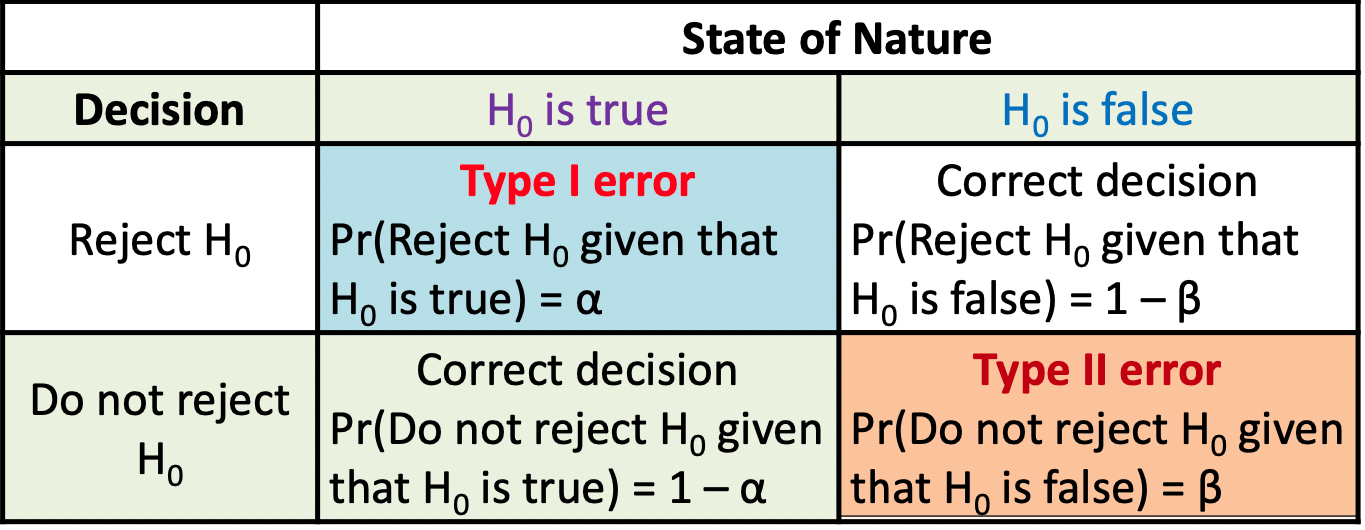
\includegraphics[width = 14cm]{Images/Types of Error.png}
    \caption{Types of Error}
    \label{fig:my_label}
\end{figure}
A \textbf{Type I} error is when you reject $H_0$ even when $H_0$ is actually true. It is considered a serious type of error. Many statisticians and experimenters fabricate data just to be able to reject the null hypothesis (and persuade people that their theory is correct). \\
A \textbf{Type II} error is not rejecting $H_0$ when $H_0$ is false. When we say that $H_0$ is false, we actually mean that $H_1$ is true. \\
Here, $\alpha$ is the level of significance. $\alpha$ is equal to the probability of making a type I error, i.e., the probability of rejecting $H_0$ even when it is true. Formally, $\alpha = P($reject $H_0|H_0$ is true$)$. \\
$\alpha$ is set by the researcher in advance (it is usually set at $5\%$ or $1\%$). \\
$\beta$ is the probability of committing a type II error, i.e., the probability of not rejecting $H_0$ even when $H_0$ is false. Formally, $\beta$ = $P($do not reject $H_0|H_1)$. \\
$$
1 - \beta = \textbf{Power of a test} = P(\textit{reject }H_0|H_1)
$$
{\color{blue} Note that it is not possible to determine the probability of committing a type II error, denoted by $\beta$, unless we have a specific alternative hypothesis.} \\
\begin{note}
\end{note}
Type I error is usually treated more seriously (since it causes a change in the status quo); so we need to control it in the first place. We set a significance level, called $\alpha$, and require that the decision rule satisfy $P($reject $H_0|H_0$ is true$) \leq \alpha$. Once we have controlled our type I error (upper bound it), we try to minimize type II error (so that our test is powerful) and so, we typically require  $P($reject $H_0|H_0$ is true$) = \alpha$. This is so that the type I error is controlled but maximized (up to an acceptable level) to reduce the type II error. Notice that when establishing a testing rule, type I and type II errors trade off each other. This similar to the trade-off between the confidence level and the width of a confidence interval - it is possible to gain confidence by expanding our interval but then it becomes meaningless. For example, if you set $\alpha = 0.0001$, i.e., your chances of making a type I error is $0.01\%$ but then your decision rule will commit a type II error with large probability.
\begin{note}
\end{note}
Observe that when a test is performed, one can make at most one type of error since if $H_0$ is rejected, type I error is possible and if $H_0$ is not rejected, then type II error is possible. These are disjoint events. 
\begin{note}
\end{note}
Hypothesis testing cannot be used to determine the truth value of any statement. It is a decision making process. Even if you reject the null hypothesis, it does not mean that the null hypothesis is false. It simply means that the evidence suggested that it was unlikely for the null hypothesis to be true. In any case, you might have made an error (which you will not find out until new evidence comes to light).
\begin{note}
\end{note}
{\color{blue}The hypotheses should not contain any random variables since it must be a statement with a fixed truth value. For example, $H_0: \bar{X} < 10$ is not a valid null hypothesis.}
\begin{note}
\end{note}
Statistical significance refers to the claim that a result from data generated by testing or experimentation is not likely to occur randomly or by chance but is instead likely to be attributable to a specific cause. A p-value less than 0.05 is statistically significant. It indicates strong evidence against the null hypothesis, as there is less than a 5$\%$ probability the null is correct (and the results are random). Therefore, we reject the null hypothesis, and accept the alternative hypothesis.
\subsection{Acceptance and Rejection Regions}
To test a hypothesis about a population parameter, we first select a suitable test statistic for the parameter under hypothesis. Once the significance level, $\alpha$, is given, a decision rule can be found such that it divides the set of all possible values of the test statistic into 2 regions, one being the rejection region (or critical region) and the other the acceptance region. \\
Once a sample is taken, the value of the test statistic is obtained. If the test statistic assumes a value in the rejection region, the null hypothesis is rejected; otherwise it is not rejected. \\
The value that separates the rejection and acceptance regions is called the critical value.

\section{Hypothesis Testing Concerning Mean}
\subsection{Known Variance}
Consider the problem of testing the hypothesis concerning the mean, $\mu$, of a population with:
\begin{enumerate}
    \item Variance, $\sigma^2$, known
    \item Underlying distribution is normal or $n$ is sufficiently large (say $n > 30$)
\end{enumerate}
\subsubsection{Two-sided Test}
Test $H_0: \mu = \mu_0$ against $H_1: \mu \neq \mu_0$. \\
When the population is normal or the sample size is large (then by the central limit theorem), we can expect that $\bar{X} \sim N\left(\mu, \dfrac{\sigma^2}{n}\right)$. Hence under $H_0: \mu = \mu_0$, we have $\bar{X} \sim N\left(\mu_0, \dfrac{\sigma^2}{n}\right)$. \\
\textbf{Critical Value Approach} \\
By using a significance level of $\alpha$, it is possible to find two critical values $\bar{x_1}$ and $\bar{x_2}$ such that the interval $\bar{x_1} < \bar{X} < \bar{x_2}$ defines the acceptance region and the two tails of the distribution $\bar{X} < \bar{x_1}$ and $\bar{X} > \bar{x_2}$ constitute the critical (or rejection region). Hence, in this case there are two cut-off values (critical values), defining the regions of rejection and acceptance. (Observe that the acceptance and rejection regions are mutually exclusive and exhaustive. This ensures that we make one of two decisions: reject $H_0$ or do not reject $H_0$.) \\
\begin{figure}[ht]
    \centering
    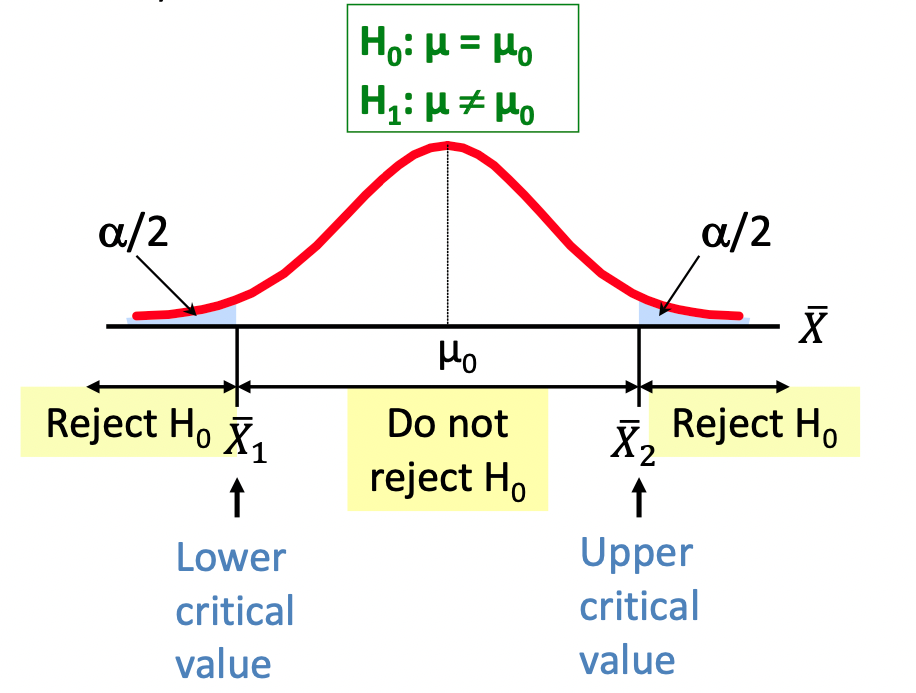
\includegraphics[width = 14cm]{Images/Two-sided test.png}
    \caption{Two-sided test}
    \label{fig:my_label}
\end{figure}
The critical region can be given in terms of z values by means of the transformation $Z = \dfrac{\bar{X} - \mu_0}{\sigma/\sqrt{n}} \sim N(0,1)$ (Note that $\mu_0$ is the value of $\mu$ under $H_0$). \\
Therefore,
$$
P\left( -z_{\alpha/2} < \dfrac{\bar{X} - \mu_0}{\sigma/\sqrt{n}} < z_{\alpha/2}
\right) = 1 - \alpha
$$
or
$$
P\left( \mu_0 -z_{\alpha/2}\dfrac{\sigma}{\sqrt{n}} < \bar{X} < \mu_0 + z_{\alpha/2}\dfrac{\sigma}{\sqrt{n}}
\right) = 1 - \alpha
$$
Hence, $\bar{x_1} =\mu_0 -z_{\alpha/2}\dfrac{\sigma}{\sqrt{n}} $ and $\bar{x_2} = \mu_0 + z_{\alpha/2}\dfrac{\sigma}{\sqrt{n}}$
From the population, we select a random sample of size $n$ and compute the sample mean. If $\bar{X}$ falls in the acceptance region $\bar{x_1} < \bar{X} < \bar{x_2}$, we conclude that $\mu = \mu_0$; otherwise we reject $H_0$ and accept that $H_1: \mu \neq \mu_0$. \\
Since $Z = \dfrac{\bar{X} - \mu_0}{\sigma/\sqrt{n}}$, therefore  $\bar{x_1} < \bar{X} < \bar{x_2}$ is equivalent to $-z_{\alpha/2} < Z < z_{\alpha/2}$. The critical region is usually stated in terms of $Z$ rather than $\bar{X}$.
\subsubsection{Relationship between two-sided test and Confidence Interval}
The two-sided test procedure just described is equivalent to finding a $(1 - \alpha)100\%$ confidence interval for $\mu$. Then, $H_0$ is accepted if the confidence interval covers $\mu_0$. If the C.I. does not cover $\mu_0$, we reject $H_0$ in favour of the alternative $H_1: \mu \neq \mu_0$ since
$$
P\left( \mu -z_{\alpha/2}\dfrac{\sigma}{\sqrt{n}} < \bar{X} < \mu + z_{\alpha/2}\dfrac{\sigma}{\sqrt{n}}
\right) = 1 - \alpha \iff P\left( \bar{X} -z_{\alpha/2}\dfrac{\sigma}{\sqrt{n}} < \mu < \bar{X} + z_{\alpha/2}\dfrac{\sigma}{\sqrt{n}}
\right) = 1 - \alpha 
$$
\begin{note}
\end{note}
{\color{blue}Confidence interval is equivalent to the hypothesis testing if, and only if, the latter is two-sided; this is applicable not only for the mean related inference but also for the variance related inference.}
\subsubsection{p-value Approach to Testing}
\begin{definition}[p-value]
p-value is defined as the probability of obtaining a test statistic more extreme (in favour of the alternative hypothesis) ($\leq$ or $\geq$) than the observed sample given the $H_0$ is true. It is also called the observed level of significance.
\end{definition}
\begin{enumerate}
    \item Convert a sample statistic to a test statistic
    \item Obtain the p-value
    \item Compare the p-value with $\alpha$. If p-value < $\alpha$, reject $H_0$. If p-value $\geq \alpha$, do not reject $H_0$.
\end{enumerate}
\begin{note}
\end{note}
Using p-value or the rejection region approach to perform the test must result in exactly the same conclusion/decision in terms of reject or do not reject $H_0$. \\
That is, p-value $ < \alpha \iff$ the test statistic is in the rejection region.
\begin{note}
\end{note}
\imp{To get the p-value for a two-sided test, 
\begin{enumerate}
    \item Take the minimum of the probability of obtaining a test statistic larger than observed value, and lower than observed value (because you don't know which is actually true: $\theta > \theta_0$ or $\theta < \theta_0$. So the more extreme one will have lower probability. Also, exactly one of $\theta > \theta_0$ or $\theta < \theta_0$ is true if the alternative hypothesis is true).
    \item Multiply this by 2 to get the p-value.
\end{enumerate}
}
\subsubsection{One-sided Test}
(a) Test $H_0: \mu = \mu_0$ against $H_1: \mu > \mu_0$. \\
Let $Z = \dfrac{\bar{X} - \mu }{\sigma/\sqrt{n}}$. Then, $H_0$ is rejected if the observed values of $Z$, say $z$, is greater than $z_{\alpha}$. Note that there is only one critical value since the rejection area is only one tail (in this case, the upper tail of the distribution).\\
(b) Test $H_0: \mu = \mu_0$ against $H_1: \mu < \mu_0$. \\
Let $Z = \dfrac{\bar{X} - \mu }{\sigma/\sqrt{n}}$. Then, $H_0$ is rejected if the observed values of $Z$, say $z$, is greater than $-z_{\alpha}$. Note that there is only one critical value since the rejection area is only one tail (in this case, the lower tail of the distribution).
\subsection{Unknown Variance}
Consider the problem of testing the hypothesis concerning the mean, $\mu$, of a population with:
\begin{enumerate}
    \item Variance unknown
    \item Underlying distribution is normal
\end{enumerate}
(1) Two-sided Test \\
 Test $H_0: \mu = \mu_0$ against $H_1: \mu \neq \mu_0$. 
 Let $T = \dfrac{\bar{X} - \mu_0}{S/\sqrt{n}}$ where $S^2$ is the sample variance. Then, $H_0$ is rejected if the observed value of $T$, say $t$, $ > t_{n - 1; \alpha/2}$ or $ < -t_{n - 1; \alpha/2}$. \\
 (2) One-sided Test \\
 Test $H_0: \mu = \mu_0$ against $H_1: \mu > \mu_0$.
 Then $H_0$ is rejected if $t > t_{n - 1; \alpha}$
 Test $H_0: \mu = \mu_0$ against $H_1: \mu < \mu_0$.
  Then $H_0$ is rejected if $t < -t_{n - 1; \alpha}$
\section{Hypotheses Testing Concerning Difference Between 2 Means}
\subsection{Known Variances}
\begin{enumerate}
    \item Variances $\sigma_1^2$ and $\sigma_2^2$ are known
     \item Underlying distributions are normal or both $n_1$ and $n_2$ are sufficiently large (greater than 30)
\end{enumerate}
We know that the difference of two normal distributions follows a normal distribution. Then, we can proceed as before using the concepts of p-value or acceptance/rejection regions.
\subsection{Large Sample Testing with Unknown Variances}
\begin{enumerate}
    \item Variances $\sigma_1^2$ and $\sigma_2^2$ are unknown
     \item Both $n_1$ and $n_2$ are sufficiently large (greater than 30)
\end{enumerate}
\subsection{Unknown but Equal Variances}
\begin{enumerate}
    \item Variances $\sigma_1^2$ and $\sigma_2^2$ are unknown but equal
     \item Both $n_1$ and $n_2$ are small (less than 30)
\end{enumerate}
\subsection{Paired Data}
\section{Hypothesis Testing Concerning Variance}
\subsection{One Variance Case}
Assume that the underlying distribution is normal. Let $X_1, X_2, \dots, X_n$ be a random sample of size $n$ drawn from a (approximate) $N(\mu, \sigma^2)$ distribution, where $\sigma^2$ is unknown. \\
We wish to test the null hypothesis $H_0: \sigma^2 = \sigma_0^2$. We know that $\chi^2 = \dfrac{(n - 1)S^2}{\sigma_0^2} \sim \chi^2(n-1)$. \\
Hence $H_0: \sigma^2 = \sigma_0^2$ is rejected if the observed $\chi^2$-value lies in the critical region (here, our test statistic is $\dfrac{(n - 1)S^2}{\sigma_0^2}$). The critical region depends on the alternative hypothesis, and is summarised as follows:
\renewcommand{\arraystretch}{1.5}
\begin{table}[h]
    \centering
    \begin{tabular}{|c|c|}
    \hline
      \textbf{$H_1$}   &  \textbf{Critical Region} \\
      \hline
        $\sigma^2 > \sigma_0^2$ & $\chi^2 > \chi_{n - 1; \alpha}^2$ \\
      \hline
        $\sigma^2 < \sigma_0^2$ &  $\chi^2 < \chi_{n - 1; 1- \alpha}^2$\\
      \hline
        $\sigma^2 \neq \sigma_0^2$ & $\chi^2 < \chi_{n - 1; 1- \alpha/2}^2$ or $\chi^2 > \chi_{n - 1; \alpha/2}^2$ \\
      \hline
    \end{tabular}
    \caption{Critical Regions for Different Alternative Hypotheses}
    \label{tab:my_label}
\end{table}
where $P(W > \chi_{n - 1; \alpha}^2) = \alpha$ with $W \sim \chi^2(n-1)$
\subsection{Ratio of Variances}
Let us assume that the underlying distribution is normal and the means are unknown.
When we are comparing the precision of one measuring device with that of another, or the variability in grading practices of one teacher with that of another, or the consistence of one production process with that of another, we are testing about the comparison between two population variances (or standard deviations). \\
We know that when two independent samples of sizes $n_1$ and $n_2$ are randomly selected from two normal populations, then $F = \dfrac{S_1^2/\sigma_1^2}{S_2^2/\sigma_2^2} \sim F(n_1 - 1, n_2 - 1)$. Under $H_0: \sigma_1^2 = \sigma_2^2$, $F = \dfrac{S_1^2}{S_2^2} \sim F(n_1 - 1, n_2 - 1)$. \\
Our test statistic is $F = \dfrac{S_1^2}{S_2^2}$. Hence $H_0: \sigma_1^2 = \sigma_2^2$ is rejected if the observed F-value lies in the critical region . The critical region depends on the alternative hypothesis, and is summarised as follows:
\renewcommand{\arraystretch}{1.5}
\begin{table}[h]
    \centering
    \begin{tabular}{|c|c|}
    \hline
      \textbf{$H_1$}   &  \textbf{Critical Region} \\
      \hline
        $\sigma_1^2 > \sigma_2^2$ & $F > F_{n_1 - 1, n_2 - 1; \alpha}$ \\
      \hline
        $\sigma_1^2 < \sigma_2^2$ & $F < F_{n_1 - 1, n_2 - 1; 1 - \alpha}$ \\
      \hline
        $\sigma_1^2 \neq \sigma_2^2$ & $F < F_{n_1 - 1, n_2 - 1; 1- \alpha/2}$ or $F > F_{n_1 - 1, n_2 - 1; \alpha/2}$ \\
      \hline
    \end{tabular}
    \caption{Critical Regions for Different Alternative Hypotheses}
    \label{tab:my_label}
\end{table}
where $P(W > F_{v_1, v_2; \alpha}) = \alpha$ with $W \sim F(v_1, v_2)$
\begin{note}
\end{note}
Test statistic plays a key role in performing hypothesis testing. Test statistic must be a function of the sample, e.g., $X_1, X_2, \dots, X_n$ and does not rely on any unknown parameter. Similar to the construction of the confidence interval, we can summarize the procedure for constructing the test statistic for mean-related hypothesis tests as follows. Denote by $\theta$ the parameter of interest. We consider the hypotheses:
$$
H_0: \theta = \theta_0 \qquad \textit{versus} \qquad H_1: \dots
$$
where $\theta_0$ is a given value \imp{which is assumed to be the true value of $\theta$ in developing the distribution of the test statistic.}
$H_1$ could be $\theta < \theta_0, \theta > \theta_0,$ or $\theta \neq \theta_0$. The following are the steps:
\begin{enumerate}
    \item Look for an estimator $\hat{\theta}$ for $\theta$, e.g., $\bar{X}$ for $\mu$.
    \item Derive the formula for $V(\hat{\theta})$.
    \item The test statistic is constructed to be $T = \dfrac{\hat{\theta} - \theta}{\sqrt{V}}$.
    \begin{enumerate}
        \item If $V(\hat{\theta})$ does not depend on any unknown parameter, e.g. when $\sigma^2$ is known, $V(\bar{X}) = \sigma^2/n$, we set $V = V(\hat{\theta})$. Then $T$ follows approximately $N(0,1)$ when the data are normal or the sample size is sufficiently large.
        \item If $V(\hat{\theta})$ contains some other unknown parameters, e.g. $\sigma^2$, we replace the parameter, e.g. $S^2$ can be used to replace $\sigma^2$ and result in $\hat{V}(\hat{\theta})$. We set $V = \hat{V}(\hat{\theta})$. Then, the distribution of $T$ has two possibilities:
        \begin{enumerate}
            \item The sample size is sufficiently large, then $T \sim N(0,1)$ approximately.
            \item If the sample size is small but the observations are normally distributed, then $T \sim t(df)$ where $df$ is the degrees of freedom of the parameter estimated in $V(\hat{\theta})$.
        \end{enumerate}
    \end{enumerate}
\end{enumerate}
Note that the above strategy is not applicable to construct test statistic for the variance related tests.
\section{Summary}
\begin{figure}[h]
    \centering
    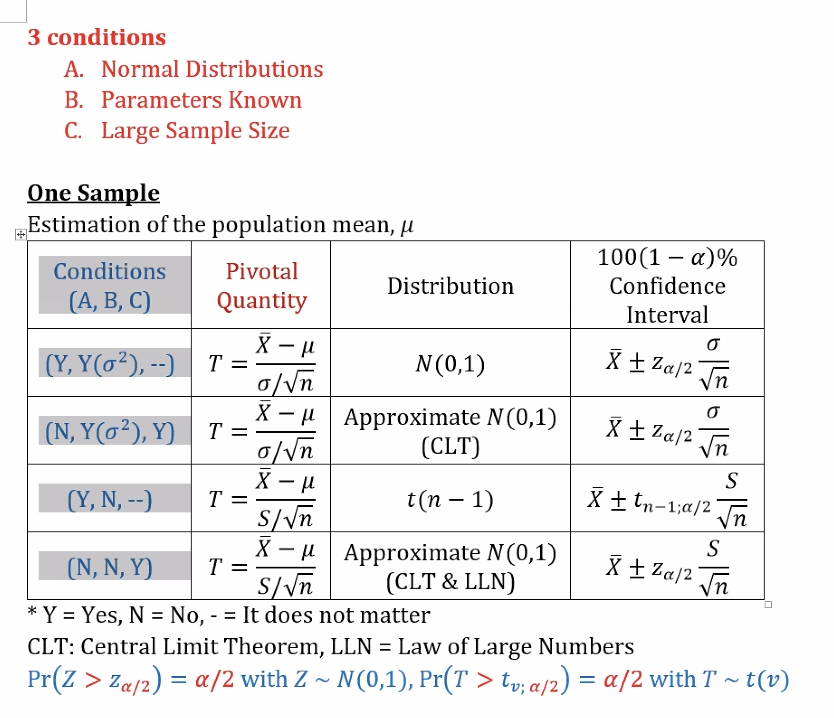
\includegraphics[width = 18cm]{Images/summary CI.png}
    \caption{Confidence Interval Summary}
    \label{fig:my_label}
\end{figure}
\begin{figure}[h]
    \centering
    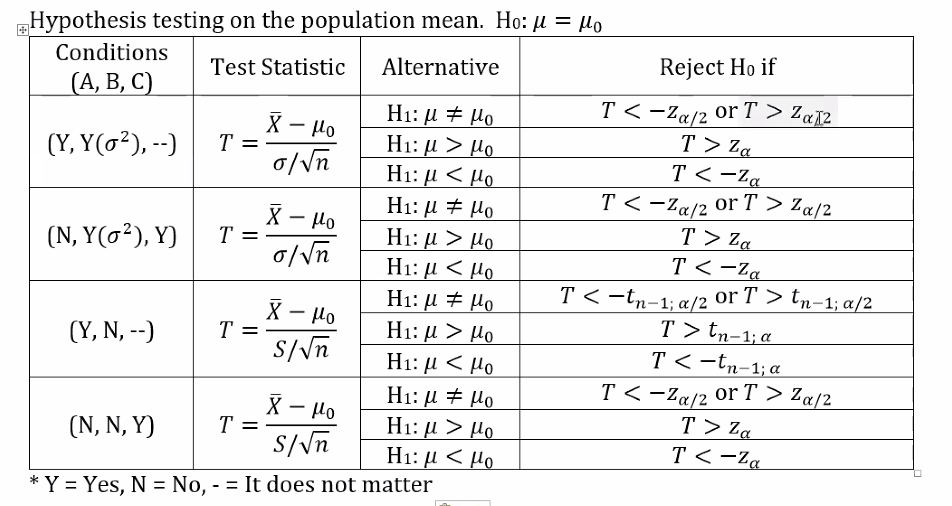
\includegraphics[width = 18cm]{Images/summary HT.png}
    \caption{Hypothesis Testing Summary}
    \label{fig:my_label}
\end{figure}
\end{document}

